%
% Template for a Thesis
%
\documentclass[a4paper,12pt,oneside]{book}
\linespread{1.2}
\usepackage[left=3.5cm, right=2.5cm, top=3.5cm, bottom=3.5cm]{geometry}
%\usepackage[latin1]{inputenc}
\usepackage[english]{babel}
\usepackage{amsfonts,amsmath,amssymb,amsthm,color}
\usepackage{graphicx}
\usepackage{float}
\usepackage{emptypage}
\usepackage{titlesec}
\usepackage{algorithm,algcompatible}
\usepackage{tabularx}
\usepackage[utf8]{inputenc}
\usepackage{subcaption}
\usepackage[hidelinks]{hyperref}
\usepackage[font=small,labelfont=bf]{caption} % caption belle alle figure
\usepackage{algorithm}
\usepackage{algpseudocode}
\usepackage{adjustbox}
\usepackage{comment}

\setcounter{tocdepth}{5}

\usepackage[
backend=bibtex,
style=ieee,
sorting=none
]{biblatex}

\addbibresource{thesis_bib.bib} % put your bibliography here

\newtheorem{theorem}{Theorem}


\raggedbottom

\graphicspath{{figs/}}

\begin{document}


%%%%%% First Page %%%

\pagestyle{myheadings}


\thispagestyle{empty}  
                                               
%\begin{center}                                                            
   % \vspace{2mm}
   % {\large ALMA MATER STUDIORUM -- UNIVERSIT\`A DI BOLOGNA} \\  

   %   \vspace{2mm}
%\end{center}
\begin{center}
	
\includegraphics[width=0.5\textwidth]{Logo_unibo.png}
\end{center}
\begin{center}
      %\vspace{5mm}
	%\vspace{2mm}
      {\large \uppercase{School of Engineering}} \\
        %\vspace{5mm}
	\vspace{2mm}
       {\large Department of\\
       Electrical, Electronic and Information Engineering\\
   		``Guglielmo Marconi''}\\
   		{\large DEI}\\
        \vspace{2mm}
      {\Large \bf Master's Degree in Automation Engineering}\\
      \vspace{2mm}
      { \textbf{Master Thesis}\\ in\\ \textit{Optimal Control}}\\
      \vspace{4mm}
      {\LARGE\bf Control of an autonomous aerodynamic airshield for training Olympic 100m sprint athletes} \\                
      \vspace{8mm}
      
      % table??
		\begin{tabularx}{\textwidth} { 
				>{\raggedright\arraybackslash}X 
				>{\raggedleft\arraybackslash}X }
				{\large Candidate:}& 	{\large Supervisor:} \\[2mm]
				{\large \itshape  Giulia Cutini} & {\large \itshape Prof. Giuseppe Notarstefano} \\[2mm]
				& {\large Co-supervisor:} \\[2mm] 
				& {\large \itshape Prof. Melanie Zeilinger} \\
                & {\large \itshape Dr. Andrea Carron} \\
                & {\large \itshape Ing. Lorenzo Sforni} \\
		\end{tabularx}
      \vfill
      {\vspace{1mm}
	\large Academic Year \\ \itshape 2022--2023} \\
      \vspace{1mm}
      {\large Session \\ \itshape III}
\end{center}


\vfill

\newpage
\thispagestyle{empty}
\mbox{}


%%%%%FRONTESPIZIO%%%%%%
\begin{center}   
	\vspace{40mm}
\end{center}

\begin{flushright}
\textit{
Alla versione più fragile di me stessa, \\
che in realtà si è sempre dimostrata \\
la più forte.}
\end{flushright} 

%%%%%% ABSTRACT %%%%%%%%%%

\newpage
\thispagestyle{empty}
\mbox{}

\chapter*{Acknowledgements }
The results presented in this thesis are the outcome of my thesis activity at the Institute for Dynamic Systems and Control (IDSC) at the ETH (Eidgen\"ossische Technische Hochschule) of Z\"urich.
The are numerous people who supported me and to whom I would like to express my gratitude.

First of all, I thank my academic supervisor Prof. Giuseppe Notastefano for his constant and important support.
Furthermore, I am grateful to the people that has supported me during the development of this thesis. 
First of all Dr. Andrea Carron for the guidance throughout the whole project. 
His suggestions during the meetings we had were crucial for every positive outcome of my master thesis.
Moreover, I am grateful to Prof. Melanie Zeilinger and Prof. Emilio Frazzoli for having hosted me in ETH, giving me the possibility of working in their Institute during the last months.
This has allowed me to make a great experience in a different country, as well as to experience both the theoretical and the practical work on MPC.


\newpage
\thispagestyle{empty}


\chapter*{Abstract}
% \addcontentsline{toc}{chapter}{Abstract}
This thesis investigates the application of modern and advanced optimal control techniques within the realm of an innovative sports application. 
Specifically, the application involves the use of an autonomous electric go-kart towing a plexiglass airshield, utilized to isolate Olympic athletes performing the 100 meters event from the drag influence during the overspeed training phase. 
The primary objective of this thesis is the deployment of a suitable controller for autonomously regulating the go-kart and the airshield in response to the position and the velocity of the runner during a sprint performance. 
The main contribution of this work lies in the development of different controllers to address the desired task: a Gain Scheduling Linear Quadratic Regulator and a Linear Model Predictive Controller. 
However, since a linear kinematic model has been used as the foundation for the controllers design, the real dynamic behaviour of the go-kart with the airshield is not perfectly described.
Specifically, the developed controllers are strongly model-based, and non-perfectly modeled dynamics effects or unknown disturbances could lead to suboptimal performance of the control architecture.  
To address this issue, an Offset-free Model Predictive Control scheme has been introduced as a third control formulation. 
To demonstrate the effectiveness of the implemented controllers, in this thesis they have been tested utilizing both Python simulations and hardware-in-the-loop tests.
A comparison of the controllers performances is presented and analyzed within the framework of Python simulations utilizing data taken from 100 meters professional athletes' competitions. 
For the hardware-in-the-loop tests on the physical system, an implementation based on the ROS 2 environment has been conducted. 
Several on-field experiments have been carried out in real-world settings to understand the performances of the controllers when operating with information coming from sensor measurements. 
This application holds significant potential for everyday use during training phases on the track and field racetrack.


%%%%%% INDEX %%%%%%%%%%


\tableofcontents



%%%%%%% BODY %%%%%%%%%

\chapter*{Introduction}
\addcontentsline{toc}{chapter}{Introduction}
\markboth{}{INTRODUCTION}
	
\section*{Motivations}
\addcontentsline{toc}{section}{Motivations}

In recent decades, the integration of advanced technologies has become an integral facet of sports, introducing a new era of innovation and performance enhancement \cite{Technology_athletics}. 
In sports characterized by high-speed competition, where victories are often determined by fractions of a second, the advancements in technology have revolutionized performance across various disciplines. 
\bigskip

The development of streamlined swimsuits with advanced materials reduces drag and enhances buoyancy, leading to faster times in competitive swimming events.
Ski manufacturers utilize materials like carbon fiber and titanium in ski construction, resulting in lighter yet more stable skis that offer better control and responsiveness on the slopes.
The incorporation of carbon fiber also into athletic footwear has not only reduced weight but also enhanced energy return and propulsion, while concurrently reducing the risk of injury.
\bigskip

The exploitation of technology to improve performances is not only used for competitions but also during the training phase. 
In the track and field context, several training techniques have been used for the enhancement of running speed. 
Among several possibilities, overspeed training involves performing exercises or movements at a velocity higher than what the athlete can achieve through voluntary effort in classical environmental conditions. 
Many methods for experiencing supramaximal velocities during training have been proposed: the usage of assistance mechanisms such as bungee cords or sleds is analized in \cite{Elastic_cord} and is found to be potentially dangerous for sprinters, requiring body contact with an external tool.
Performing sprints on a downward slope allows athletes to accelerate beyond typical maximal speed due to assistance provided by gravity force \cite{Hill_slope}.
\bigskip

In the context of gaining a training edge in sprint events, the concept of aerodynamic drag resistance assumes a great importance. 
Accordingly sprinters meticulously refine their body position, posture, and apparel to minimize aerodynamic drag. 
For this reason CONI (Italian National Olympic Committee) Institute of Sports Science presented in 2021 an aerodynamic shield to drastically reduce the resistance to forward movement during sprinters' training \cite{Coni_article}. 
This shield allows athletes to run in the slipstream behind a car pulling the shield, experiencing speeds higher than those of the competition but with the same power output. 
\bigskip

Advancements in automated driving technology have created opportunities for many fields, and autonomous vehicles (AVs) have become increasingly prevalent. 
Given their versatility and potential to enhance efficiency and convenience, it's natural to consider their application in the realm of sports. 
Similarly to user-cooperative robots, designed to stay in direct contact with humans and assist them in several situations, an autonomous vehicle has been designed for driving the aerodynamic airshield. 
Furthermore, intelligent control algorithms have shown huge advantages in autonomous system control, taking into account factors such as control error, bound constraints on system actuators, disturbance rejection and safety guarantees. 
Additionally, control algorithms can be designed to continuously monitor and analyze data from various sensors in real-time, enabling them to detect and respond to potential hazards or deviations from safety protocols more effectively than human operators.
\bigskip

This thesis is the result of an abroad internship in ETH (Eidgen\"ossische Technische Hochschule) Z\"urich, with the purpose of designing a proper controller to regulate an autonomous go-kart pulling a plexiglass airshield, according to the runner's behaviour.

		
\section*{Literature}
\addcontentsline{toc}{section}{Literature}
Numerous control techniques have been used in recent decades to enhance the efficiency of AVs in several different contexts.
Longitudinal control of automated vehicles has received attention since the 1960s, and possibly even earlier.
In \cite{Review_AVCS}, a historical review of advanced vehicle control systems and longitudinal control of automated vehicles is presented.
The control of vehicle acceleration to achieve a desired speed profile, an essential key point of longitudinal control, is the main purpose of this thesis.

\bigskip
The initial and simplest approach adopted to control the go-kart, which must maintain a constant reference position and velocity relative to the runner behind it, involved a cascade of two Proportional-Integral-Derivative (PID) controllers.
The first PID controller regulates the kart's position and generates a reference velocity for the second controller, a velocity PID.

While PID controllers are widely used in industrial applications due to their straightforward implementation, they were not the optimal choice for this application.
The main challenges of this control scheme include difficulty in parameter tuning, in handling multi-variable processing, and in addressing the initial phase of motion, where the runner's acceleration exceeds the kart's maximum capability, together with the impossibility of predicting the future motion of vehicle. 

\bigskip
The application requires the go-kart to maintain a consistent desired position and velocity relative to the runner.
This task is quite similar to adaptive cruise control (ACC), where the goal is to maintain a safe distance from the vehicle ahead while also adjusting the speed to match changing traffic conditions.

\bigskip
Thanks to the capability of optimal controllers to cover multiple objectives and to predict future vehicle behaviour, Linear Quadratic Regulator (LQR) and Model Predictive Control (MPC) have been widely used for vehicle control in interacting contexts.
In \cite{LQR_acc}, distance and relative velocity between preceding and controlled vehicles are used as states to design an LQR controller that gives acceleration of the controlled vehicle as input, in such a way to minimize a proper cost function.
Model Predictive Control is also largely used thanks to its capability of controlling a multi-variable process while satisfying a set of state and input constraints. 
According to \cite{MPC_basics}, the essential elements of this controller are a prediction model that allows future predictions, the definition of an objective function reflecting the desired system behaviour, and constraints on both state and input. 
In the framework of MPC for adaptive cruise control, in \cite{MPC_acc_first}, the same state and input variables than in \cite{LQR_acc} are used but constraints can be also incorporated. 
Differently, in \cite{MPC_acc_second}, the controlled vehicle's velocity is added as a third state and the acceleration of the preceding vehicle is included in the prediction model, regarded as an unknown external disturbance.

\bigskip
The MPC approach is strongly model-based in the sense that uses a model of the system to produce predictions of the system behaviour. 
The presence of uncertainties in this model may lead to unsatisfying results of the control task. 
For this reason, \cite{Offset-free_compare, Linear_offset-free} show offset-free MPC formulations able to achieve output tracking of reference signals despite the presence of Model-Plant Mismatch (MPM).
For this purpose an augmented predictive model added with an artificial constant disturbance that represents modeling uncertainties is used. 
To estimate both state ad disturbance from output measurements a disturbance observer must be properly designed and added in conjunction with feedback control law.
Accordingly to \cite{Disturbance_observer}, by appropriately including a disturbance estimate in a control law, MPM effects can be approximately removed in steady-state and offset-free tracking of constant references can be achieved.


	
\section*{Contributions}
\addcontentsline{toc}{section}{Contributions}
The main contribution of this thesis lies in the analysis and implementation of linear controllers for an innovative autonomous driving go-kart, which is used to tow the airshield during the training of Olympic athletes participating in the 100 meters event.
Specifically, the thesis proposes and compares three different control schemes in terms of performances and control architecture.

\bigskip
A linear kinematic model approximating the go-kart and the airshield dynamic behaviour has been utilized as the basis for the design of the predictive controllers.
This linear model approximates, based on simplifying assumptions, a more complex nonlinear model.
The first step in control development involves the design of a Linear Quadratic Regulator (LQR) with a gain scheduling approach, where Q and R parameters vary depending on the motion phase. 
This gain scheduling approach addresses the challenges associated with the different maximum accelerations of the kart and of the runner in the first phase of motion.
Subsequently, a Model Predictive Control (MPC) is designed with the purpose of incorporating information on the runner's future expected behaviour into the linear prediction model.
Furthermore, since MPC is highly model-based, a disturbance observer and Offset-free MPC have been implemented with the purpose of increasing the accuracy of the predictive model and obtaining a zero-offset in tracking piece-wise affine (PWA) reference trajectories.

\bigskip
The depicted workflow highlights how the control scheme architecture has been simplified starting from the two control loops governing the cascade of PID controllers. 
The gain scheduling LQR, which switches between two different control gains depending on the motion phase, just makes use of two different regulators. 
Ultimately, this thesis culminates in a single MPC controller capable of governing the system under all possible operating conditions, integrating information about the future evolution of the runner's velocity profile into the prediction model to further enhance tracking performance.

\bigskip
Both controllers have been developed and tested in simulation using Python and on the real system using ROS2 environment.

\section*{Organization}
This section provides to the reader a guide to the organization of the thesis. 

In Chapter 1 a theoretical background and an overview of the fundamental optimal control theory and methodologies used in the control design are presented. 

Chapter 2 is focused on discussing the problem set-up, in presenting a proper linear approximation of the system dynamics and in the formulation of the optimal control techniques to accomplish the desired task, in particular the Linear Quadratic Regulator (LQR) and the Model Predictive Control (MPC), in the specific context of this application.

Chapter 3 shows the numerical results of the controllers application obtained in Python simulation environment. A comparison of the performances in different scenarios is presented.

Chapter 4 gives a description of the system mechanical structure, hardware and sensors. The hardware-in-the-loop tests based on a ROS2 implementation and conducted in a real-world scenario are presented and discussed.
This demonstrate the real effectiveness of the proposed methodologies.

\chapter{Optimal Control theory: Linear Quadratic Regulator and Model Predictive Control for controlling dynamical systems}
%\addcontentsline{toc}{chapter}{Theoretical Background}
\markboth{}{OPTIMAL CONTROL OF DYNAMICAL SYSTEMS}
%\label{chapter:Theoretical_Background}
In this chapter the aim is to provide the necessary theoretical background in optimal control before introducing the design process, as well as the main peculiarities and limitations of the implemented controllers: the Linear Quadratic Regulator (LQR) and the Model Predictive Control (MPC).

Optimal control theory provides a mathematical framework for addressing control theory problems by optimizing control laws with respect to given cost functions, in order to achieve optimal system regulation.

Such theoretical analysis is essential for fully comprehending the features and performances of the LQR and MPC controllers discussed later in Chapter 2 within the specific context of the considered application.

\section{Linear Quadratic Regulator}
In 1960, Kalman introduced for the first time the linear-quadratic feedback control, which later evolved into the Linear Quadratic Regulator (LQR) \cite{kalman_contributions} in the continuous-time context. 
The LQR is a feedback control algorithm designed to stabilize and optimize the performance in cases where the dynamical system can be described by linear equations and the cost function is quadratic in terms of the states and inputs. 

\bigskip
Assuming that the process to be controlled can be described by a discrete-time LTI dynamical system, such as the following state-space form:
\begin{equation} 
\begin{aligned}
    x_{t+1} &= A x_t + B u_t \\
    y_t &= C x_t
\end{aligned}
\label{eq:Linear_model}
\end{equation}

where $x_t \in \mathbb{R}^n$ is the actual system state, $u_t \in \mathbb{R}^m$ is the system input and $y_t \in \mathbb{R}^p$ is the measured output, all considered at a certain discrete time instant $t$. 
The state at the subsequent time instant $t+1$ is referred to as $x_{t+1}$.

$A \in \mathbb{R}^{n\times n}$ and $B\in \mathbb{R}^{n\times m}$ are the state and input matrices, respectively.
In the context of this thesis, it is possible to assume the full state information is available, thus the input matrix $C \in \mathbb{R}^{p\times n}$ is the identity. 

\bigskip
The main goal of the control task is to achieve optimal regulation of the system's states towards the origin. 
The notion of optimality, in this context, is framed within a quadratic objective function.
The LQR problem, therefore, can be viewed as a multi-objective optimization task, where the goal is to simultaneously minimize competing objectives.
For example, minimizing the deviation of the system's states from desired values may require higher control effort, and vice versa.
In the context of multi-objective optimization, the challenge lies in finding a balance between these conflicting objectives and this always involves making trade-offs to achieve a satisfactory solution.

\bigskip
The Infinite Horizon Linear Quadratic Regulator problem is defined as follows:
find the optimal control input $u_t, \, \forall t \in [0, \infty)$ that makes the following quadratic criteria as small as possible
\begin{equation}
    J(\boldsymbol{x}, \boldsymbol{u})  = \sum_{t=0} ^{+\infty} x_t^\top Q x_t + u_t ^\top R u_t
\label{Quadratic_cost_funct}
\end{equation}
where $Q \in \mathbb{R}^{n \times n}$ and $R \in \mathbb{R}^{m \times m}$ are symmetric positive-definite weight matrices.

The vector $\boldsymbol{u}$, also known as input trajectory, consists of the input elements, i.e. $\boldsymbol{u} = \{u_0, u_1, \dots\}$ and $\boldsymbol{x}$, the state trajectory, consists of the states along the infinite time horizon, i.e $\boldsymbol{x} = \{x_1, x_2, \dots\}$.
The cost function in \eqref{Quadratic_cost_funct} can be seen as the mathematical formulation of the trade-off between the two objectives to be minimized.
Specifically, the term $x_t^\top Q x_t$ penalizes deviations of the system's states from desired values, while $u_t^\top R u_t$ penalizes excessive control effort.
The weights of $Q$ and $R$, typically chosen as diagonal matrices, can be adjusted to find solutions that strike an appropriate balance between minimizing state deviations and control effort.

\bigskip
The overall LQR problem can be mathematically translated into the following optimization problem:
\begin{equation}
\begin{aligned}
	\min_{\substack{\boldsymbol{x}, \boldsymbol{u}}}\quad & \sum_{t=0}^{+\infty}  x_t ^\top Q x_t  + u_t^\top R u_t  \\
	\text{subj. to} & \quad x_{t+1}  = A x_t + B u_t \hspace{2cm} t = 0, 1 \ldots. \\
    & \quad x_0 = x_{\text{init}}
\end{aligned}
\label{eq:LQR_1}
\end{equation}
where  $x_{\text{init}} \in \mathbb{R}^n$ is the initial condition of the system at time $t=0$.



\bigskip
Assuming the pair $(A,B)$ to be controllable and the pair $(A,C)$ with $Q = C^\top C$ to be observable, the following holds:
\begin{itemize}
    \item there exists a unique positive definite $P_\infty$ solution of the following equation called Algebraic Riccati Equation (ARE)
    \begin{equation}
        P_\infty = Q + A^\top P_\infty A - A^\top P_\infty B (R + B^\top P_\infty B)^{-1} B^\top P_\infty A.
    \end{equation}
    \item exploiting the first-order necessary and sufficient conditions for optimality, the optimal control law is a closed-form solution, feedback of the state
    \begin{equation}
        u_t^* = K x_t^*
    \end{equation}
    with
    \begin{equation}
        K = -( B^\top P_\infty B + R)^{-1}(B^\top P_\infty A)
    \label{eq:Regulator_LQR}
    \end{equation}
    and it is able to asymptotically stabilize the system.
\end{itemize}

The pair $(x_t^*, u_t^*)$ is the optimal state and input at discrete time instant $t$.

\bigskip
Despite the fact that one of the main applications of LQ optimal control is regulation, this strategy can be used to track a desired system behaviour as closely as possible, in the framework of Linear Quadratic Tracking (LQT) \cite{Linear_Quadratic_Tracking}.
To incorporate the desired behaviour to be tracked in the objective, the problem can be written as:
\begin{equation}
\begin{aligned}
	\min_{\substack{\boldsymbol{x}, \boldsymbol{u}}}\quad & \sum_{t=0}^{+\infty}  (x_t - x_{t,\text{des}})^\top Q (x_t - x_{t,\text{des}}) + u_t^\top R u_t  \\
	\text{subj. to} & \quad x_{t+1}  = A x_t + B u_t \hspace{2cm} t = 0, 1 \ldots. \\
    & \quad x_0 = x_{\text{init}}
\end{aligned}
\label{eq:LQR}
\end{equation}

where $x_{t,\text{des}} \in \mathbb{R}^n$ is the reference state value we want our system's states to track at time $t$.

The cost function quantifies the controlled system's performance, defined as a weighted sum of the deviations of the system's states from desired values and control effort.

In the context of tracking a given desired state behaviour $x_{\text{des}}$ the optimal feedback control law is modified in the following way:
\begin{equation}
    u_t^* = K (x_t - x_{t,\text{des}})
\label{Closed-loop_control_law}
\end{equation}
where the term $x_t - x_{t,\text{des}}$ is the tracking error at time $t$.

The effectiveness of LQR lies in its ability to leverage the full state information of the system, enabling precise and efficient control.


\section{Linear Model Predictive Control}
Model Predictive Control (MPC) is a modern control strategy well known for its capacity to provide optimized responses while accounting for state and input constraints, such as saturation limits.
These constraints can be explicitly integrated into the control design, enhancing the robustness and performance of the system. 
The origin of MPC trace back to the mid-seventies to mid-eighties, initially emerging in industrial applications. 
However, it was not until the nineties that MPC theory underwent significant advancements, leading to its widespread adoption and refinement.

\bigskip
MPC relies on the provided dynamic model to predict the behaviour of the system and determine the optimal control action based on the chosen performance criteria. 
A key aspect of MPC design is selecting a suitable model, one that adequately describes the system's dynamics while maintaining simplicity to ensure tractability and real-time solvability of the optimization problem.

\bigskip
The description of the linear discrete-time system prediction model is the same shown in \eqref{eq:Linear_model}.

For what regards the states and inputs constraints they can be expressed as follows
\begin{align}
    x_t & \in \mathcal{X} \quad \quad \forall t = 0,1, \ldots \\
    u_t & \in \mathcal{U} \quad \quad \forall t = 0,1, \ldots
\end{align}
where the state set $\mathcal{X}$ is closed and the input set $\mathcal{U}$ is compact and non-empty. 
Usually, the sets are described with linear inequalities, and both sets are convex and contain the origin.

\bigskip
Similarly to the LQR case, Model Predictive Control aims to minimize a cost function by defining positive definite matrices $Q$ and $R$. 
The goal is to find the optimal control input that minimizes a cost function, taking the following form:
\begin{equation}
    J(\boldsymbol{x}, \boldsymbol{u}; x_t, t) = \sum_{i=t} ^{+ \infty} x_{i|t}^\top \, Q \, x_{i|t} + u_{i|t}^\top \, R \, u_{i|t}
\end{equation}

In this formulation, $x_{i|t}$ represents the predicted state a time $i$, given the initial state $x_t = x_{t|t}$. 
Similarly, $u_{i|t}$ is the predicted control sequence at current time $t$ found by considering the entire future predicted trajectory for the system.

\bigskip
The aforementioned formulation represents the infinite horizon MPC problem, which in many practical cases results challenging to be implemented or requires highly demanding computations.
For this reason, usually MPC formulations optimize only on a finite horizon $N$, thus the problem of tracking $x_{\text{des}}$ with the system's states becomes:

\begin{equation}
\begin{alignedat}{2}
	\min_{\substack{\boldsymbol{x}, \boldsymbol{u}}}\quad & \sum_{i=t}^{t+N-1} (x_{i|t} - x_{t,\text{des}}) ^\top \, Q \, (x_{i|t} - x_{t,\text{des}}) +  u_{i|t}^\top \, R \, u_{i|t} &&   \\
	\text{subj. to} & \quad x_{i+1|t}  = A x_{i|t} + B u_{i|t}   \hspace{2cm} t = 0, 1 \ldots N &&  \\
     &\quad x_{i|t} \in \mathcal{X} && \\
    &\quad u_{i|t} \in \mathcal{U} && \\
    &\quad x_{t|t} = x_{\text{meas}}(t) && 
\end{alignedat}
\label{MPC1}
\end{equation}

\begin{figure}
	\centering
	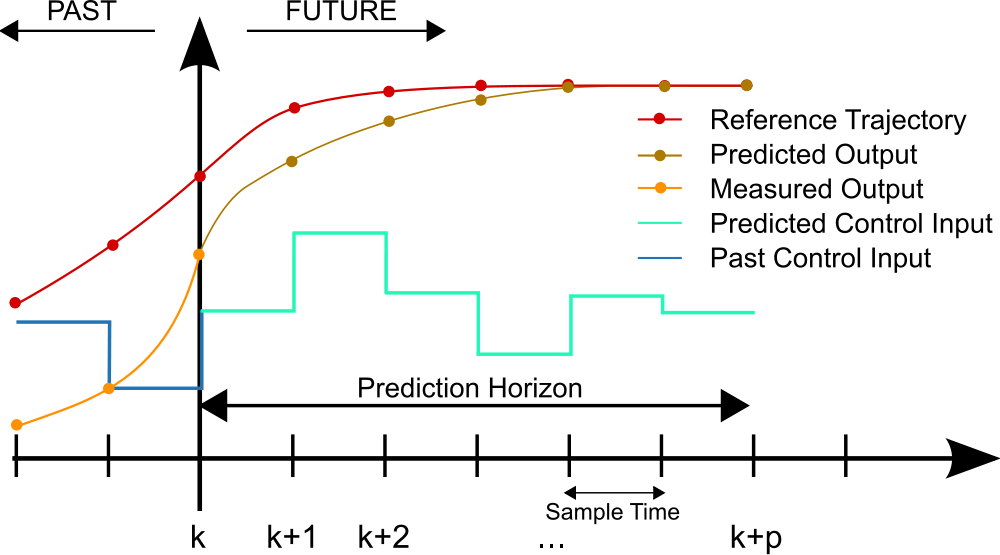
\includegraphics[width=0.66\textwidth]{MPC.png}
	\caption{Model Predictive Control receiding horizon scheme}
	\label{image:mpc}
\end{figure}

\bigskip
The control law is applied based on the receding horizon principle, which is a key feature of MPC.
This principle dictates that at each time instance $t$, an open-loop optimal control problem is solved using the current state of the plant $x_{\text{meas}}$ as the initial state for the optimization problem, in order to obtain the control action. 
All predicted states and inputs within a prediction horizon $N$ are optimized to find an optimal input sequence.
However, only the first input of the optimal control sequence generated by the optimization is injected into the plant. 
This input is used to control the system over the next time step.
This procedure is repeated, as illustrated in figure \ref{image:mpc}, at each time instance, and by continuously updating the control action based on the most recent information, MPC ensures that the control strategy adapts to changes in the system dynamics and external conditions over time.




\section{Offset-free Model Predictive Control and Disturbance Observer}
Regulating nonlinear systems using a linear predictive control framework can be a complex task and the model-plant mismatch due to the unmodeled nonlinear dynamics effects, can result in suboptimal performances of the controller.

\bigskip
Even if MPC is able to react to small unmodeled dynamics effects through its receding-horizon fashion,it does not inherently incorporate them into its predictions or optimization.
As a consequence, MPC solves an optimal control problem at each time step using the nominal model of the controlled process. 
Only when the actual plant behavior closely matches the nominal model can the feedback control scheme be guaranteed to stabilize the system and achieve precise tracking of desired setpoints without any offset.

\bigskip
Offset-free Model Predictive Control represents an advanced control strategy designed to address this limitation. 
Its objective is to achieve zero steady-state tracking errors in the controlled system, even in the presence of disturbances or model uncertainties causing model-plant mismatch.
For instance, in the context of regulating nonlinear systems using a linear predictive control framework, offset-free MPC seeks to regulate the system to its desired setpoint without steady-state error, ensuring precise and accurate control performance.

\bigskip
Consider a discrete-time, time-invariant system describing the plant:
\begin{equation}
\begin{aligned}
    x_{m,t+1} &= f_m (x_{m,t}, u_t) \\
    y_{m,t} &= h_m (x_{m,t}) 
\end{aligned}
\label{Plant1}
\end{equation}
where $x_{m,t} \in \mathbb{R}^n$, $u_t \in \mathbb{R}^m$ and $y_{m,t} \in \mathbb{R}^p$ are the state, input and measured output of the plant at time $t$, respectively.

The aim of the offset-free model predictive controller is to have $y_m$ tracking a certain reference signal $y_{\text{des}} \in \mathbb{R}^p$ that is assumed to asymptotically converge to a constant.

\bigskip
Let $w \in \mathbb{R}^n$ and $v \in \mathbb{R}^p$ be defined as follows:
\begin{equation}
\begin{aligned}
    w & := f_m (x_m, u_t) - (A x + Bu) \\
    v & := h_m (x_m) - C x
\end{aligned}
\label{Plant_model_mismatch}
\end{equation}
Here, $w \in \mathbb{R}^n$ represents the model mismatch between the nonlinear plant model and the linear predictive model, while $v \in \mathbb{R}^m$ represents the output mismatch between the predicted output and the real measured plant output.
The $A$, $B$ and $C$ matrices are the ones mentioned in the linear model \eqref{eq:Linear_model}.

\bigskip
The key feature of this offset-free control strategy lies in the incorporation of a disturbance model in the prediction model \eqref{eq:Linear_model}.
This disturbance allows to capture the mismatch between the linear prediction model \eqref{eq:Linear_model} and the nonlinear plant \eqref{Plant1} in steady state, thus the $w$ term, and to consider it inside the optimization.

The steps to be followed to obtain an offset-free MPC formulation are the following:
\begin{enumerate}
	\item Introduce an augmented prediction model with an additional integrating state known as disturbance, to model the model-plant mismatch
	\item Design a state and disturbance estimator based on the augmented model
	\item Modify the MPC formulation into an offset-free one, considering the estimated disturbance in the formulation
\end{enumerate}
Each point will be properly explained in detail in the following.

\subsection*{Augmented model with disturbance}
As mentioned earlier, the first step is to introduce an augmented model for computing the system's predictions in the offset-free MPC framework. 
This augmented model can generally be written in the following form:
\begin{equation}
\begin{aligned}
    x_{t+1} &= A x_t + B u_t + B_d d_t \\
    d_{t+1} &= d_t \\
    y_t &= C x_t + C_d d_t
\end{aligned}
\label{Augmented_model}
\end{equation}
where the additional state $d_t \in \mathbb{R}^{n_d}$, known as disturbance state or simply disturbance, is assumed to be constant and follows an integral dynamics, as proposed by \cite{pannocchia2003disturbance}. 
The pair $(B_d, C_d)$, where $B_d \in \mathbb{R}^{n \times n_d}$ and $C_d \in \mathbb{R}^{m \times n_d}$, can be seen as the disturbance model matrices.
The maximum dimension of the disturbance state must be equal to the number of measured outputs, i.e. $n_d \leq p$.

\subsection*{Disturbance observer and estimator}
Assuming observability of the augmented system \eqref{Augmented_model}, an estimator that continuously estimates the augmented state $(x,d)$ can be designed.
An example could be a linear disturbance observer, which uses the prediction error between the real plant output and the predicted one to estimate the augmented state.
This can be described by the following dynamical system:
\begin{equation}
    \begin{aligned}
    	\begin{bmatrix}
    	   \hat{x}_{t+1} \\
            \hat{d}_{t+1}
        \end{bmatrix}
        &= 
    	\begin{bmatrix}
    		A & B_d \\
    		0 & I
    	\end{bmatrix}
    	\begin{bmatrix}
    		\hat{x}_t \\
    		\hat{d}_t
    	\end{bmatrix}
        +
    	\begin{bmatrix}
    		B \\
    		0
    	\end{bmatrix}
        u +
        \begin{bmatrix}
            L_x \\
            L_d \\
        \end{bmatrix} 
        ( - y_{m,t} +
        \begin{bmatrix}
            C & C_d 
        \end{bmatrix}
        \begin{bmatrix}
            \hat{x}_t \\
            \hat{d}_t
        \end{bmatrix} ) \\
        & = A_e 
        \begin{bmatrix}
        \hat{x}_t \\
        \hat{d}_t
    	\end{bmatrix}
        + 
        B_e \, u +
        L (
         - y_{m,t} +
        C_e
        \begin{bmatrix}
            \hat{x}_t \\
            \hat{d}_t
        \end{bmatrix} )
    \end{aligned}
\label{eq:Estimator_and_observer}
\end{equation}
where $\hat{x} \in \mathbb{R}^n$ and $\hat{d} \in \mathbb{R}^{n_d}$ are the state and disturbance estimates.

The matrices $A_e \in \mathbb{R}^{(n+n_d) \times (n+n_d)}$, $B_e \in \mathbb{R}^{(n+n_d) \times m}$ and $C_e \in \mathbb{R}^{p \times (n + n_d)}$ are the following:
\begin{equation}
    A_e =
    \begin{bmatrix}
        A & B_d \\
        0 & I  
    \end{bmatrix},
    \quad
    B_e = 
    \begin{bmatrix}
        B \\
        0  
    \end{bmatrix},
    \quad
    C_e = 
    \begin{bmatrix}
        C & C_d 
    \end{bmatrix}.
\end{equation}
The $L \in \mathbb{R}^{(n+n_d) \times p}$ matrix is described as follows:
\begin{equation}
    L =
    \begin{bmatrix}
        L_x \\
	L_d 
    \end{bmatrix}
\end{equation}

The system in \eqref{eq:Estimator_and_observer} estimates, at each time instant $t$ the unknown disturbance (i.e. the model-plant mismatch in this context) in addition to the plant states. 
The estimation is performed evaluating the prediction error between the measured plant output and the predicted one.

\subsection*{Offset-free MPC formulation}
Given the current estimates of the augmented state $(\hat{x}_t, \hat{d}_t)$ at discrete time $t$, the classical MPC formulation is modified into an offset-free MPC formulation.

The estimated variables  $(\hat{x}_t, \hat{d}_t)$ are used as initial states for the MPC optimization problem at the current solving time instant $t$.
The augmented model in \eqref{Augmented_model} is employed as prediction model: the disturbance is included both as a constant state and in the state evolution equation.

The resulting formulation is the following one:
\begin{equation}
\begin{alignedat}{2}
	\min_{\substack{\boldsymbol{x}, \boldsymbol{u}}}\quad & \sum_{i=t}^{t+N-1} (x_{i|t} - \bar{x}_t) ^\top \, Q \, (x_{i|t} -  \bar{x}_t) +  (u_{i|t} - \bar{u}_t)^\top \, R \, (u_{i|t} - \bar{u}_t) &&  \\
	\text{subj. to} & \quad x_{i+1|t}  = A x_{i|t} + B u_{i|t} + B_d d_{i|t} \hspace{1.5cm} t = 0, 1 \ldots N &&  \\
    & \quad d_{i+1|t}  = d_{i|t} && \\
    &\quad x_{i|t} \in \mathcal{X} &&  \\
    &\quad u_{i|t} \in \mathcal{U} && \\
    &\quad x_{t|t} = \hat{x}_t && \\
    &\quad d_{t|t} = \hat{d}_t && 
\end{alignedat}
\label{MPC:offset-free}
\end{equation}
where $\bar{x}_t \in \mathbb{R}^n$ and $\bar{u}_t \in \mathbb{R}^m$ are solution of the following system:

\begin{equation}
    \begin{bmatrix}
    A-I & B \\
    C & 0
	\end{bmatrix}
 	\begin{bmatrix}
		\bar{x}_t \\
		\bar{u}_t
	\end{bmatrix}
    =
    \begin{bmatrix}
    -B_d \hat{d}_t\\
    y_{\text{des}} - C_d \hat{d}_t
	\end{bmatrix}
\end{equation}

In this system, the coefficient matrix or left-hand side matrix, represents the dynamics of the system according to the linear model (i.e. the $(A, B, C)$ matrices), while the right-hand side vector incorporates the disturbance model (i.e. the $(B_d, C_d)$ matrices), the estimated disturbance $\hat{d}$ and the desired plant reference setpoint $y_{\text{des}}$.
This system may be in general overconstrained, implying that there may not exist a solution that satisfies all equations exactly.
In this cased the solution is typically found using the least square method with the pseudoinverse.

\subsection*{Luenberger observer design}
%\addcontentsline{toc}{section}{Observer design}

In this offset-free MPC formulation, the nominal augmented state $(x,d)$ needs to be estimated at each time instant, given the plant output measurement $y_m$, according to the dynamical estimator system in \eqref{eq:Estimator_and_observer}.

The $L_x \in \mathbb{R}^{n \times p}$ and $L_d \in \mathbb{R}^{n_d \times p} $ observer gain matrices in \eqref{eq:Estimator_and_observer} need to be designed in such a way the estimator to be stable, while the method doesn't matter for our purposes.

\bigskip
Two possible common choices for state estimators are the Luenberger observer and the Kalman filter. 
Specifically, in the context of this thesis, the Luenberger observer has been employed.
It updates the state prediction computed at time $t-1$ using the current measured plant output $y_m$ at time $t$ as in the following:
\begin{equation}
    \hat{x}_t = A \hat{x}_{t-1} + B u_{t-1} + L (y_{m,t} - \hat{y}_t)
\end{equation}
where $\hat{y}_t := C(A \hat{x}_{t-1} + B u_{t-1})$.
The difference $(y_{m,t} - \hat{y}_t)$ is referred to as the estimation error or correction term, and $L \in \mathbb{R}^{n \times p}$ is the observer gain.

\bigskip
If the pair $(A_e,C_e)$ in \eqref{eq:Estimator_and_observer} is observable, than the eigenvalues of $(A_e+LC_e)$ can be placed arbitrarily to ensure stability of the estimator dynamical system.
Typically, the desired eigenvalues for $(A_e+LC_e)$, i.e. the poles of the estimator dynamical system, are chosen to be smaller than those of the controlled stabilized system to ensure the estimator to be faster than the controller.

\chapter{Design of Optimization-based Controller for autonomous airshield}
%\addcontentsline{toc}{chapter}{Control design}
\markboth{}{CONTROL DESIGN}
\label{chapter:Control_design}
This chapter will begin with a description of the go-kart plant model and its linear approximation, which is utilized in the design of the predictive controllers. 

Later on, a detailed description and explanation of the design choices and formulations of both the controllers within the context of the sport application: the Linear Quadratic Regulator (LQR) and the Model Predictive Control (MPC), nominal and with Offset-free version.

\section{Go-kart kinematics model}
\begin{figure}[h!]
	\centering
	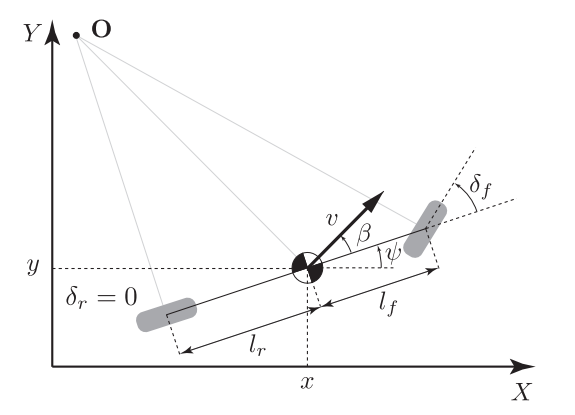
\includegraphics[width=0.7\textwidth]{Bycicle_scheme.png}
\caption{Kinematic bicycle model of the vehicle}
\label{Kinematic_bicycle}
\end{figure}
%Having a good model plays a central role in the controller design framework.
The non linear model utilized to describe the motion of the go-kart is a bicycle kinematic model, illustrated in figure \ref{Kinematic_bicycle}.
The 2D bicycle model can be seen as a simplified car-like vehicle model that closely approximates the motion of a four-wheel vehicle in normal driving conditions.

The mathematical equations are the following:
\begin{equation}
\begin{cases}
 	\begin{aligned}
		\dot{x}(t) &= v(t) \cos(\psi(t) + \beta(t)) \\
		\dot{y}(t) &= v(t) \sin(\psi(t) + \beta(t)) \\
		\dot{\psi}(t) &= \frac{v(t)}{l_r} \sin(\beta(t)) \\
		\dot{v}(t) &= \frac{F_x(t)}{m} 
	\end{aligned}
\end{cases}
\label{Plant}
\end{equation}

where $x = [x, y, \psi, v]$ is the state vector, where the components are respectively the $x$ and $y$ world frame coordinates, $\psi$ is the heading angle with respect to the reference frame, and $v$ is the total speed of the vehicle.

The longitudinal force $F_x$ acting on the vehicle is modeled as a single force applied to the center of gravity and is computed as a combination of the drive-train command and the velocity. 
\begin{align}
    F_x (t) &= (C_{m_1} - C_{m_2} v(t)) a(t) - C_f v(t) - C_d v^2(t) - C_{roll} \label{eq:Long_force}\\
    \beta(t) &= \arctan\left(\tan\left(\frac{l_r}{l_f+l_r}\delta_f(t)\right) \right).
\end{align}
The inputs of this system are $u = [a, \delta_f]$ where $a$ is the drive-train acceleration and $\delta_f$ is the front steering angle. 
The variable $\beta$ represents the slip angle at the center of mass. 

\bigskip
The model has two parameters, $l_f$ and $l_r$, which represent the distances from the centre of mass to the front axle and rear axle, respectively.

The mass $m = 300$ Kg includes both the kart and the trailer weight, while $l_f = l_r = 0.8$ meters.
The other parameters of this model have been identified as reported in table \ref{tab:Parameters}.


\bigskip
The identified coefficients represent:
\begin{itemize}
    \item $C_{roll}$ : rolling coefficient modeling the wheel friction on the road surface
    \item $C_d$ : coefficient modeling aerodynamic resistance or drag
    \item $C_f$ : coefficient modeling the dynamic friction resistance
    \item $C_{m1}$ : coefficient associated with the force component due to the driving torque of the vehicle
    \item $C_{m2}$ : coefficient associated with the force component due to both the torque and the velocity
\end{itemize}

\begin{table}[h!]
    \centering
    \begin{tabular}{|c|c|}
        \hline
        $C_{m1}$ & 930 \\
        \hline
        $C_{m2}$ & 0 \\
        \hline
        $C_f$ & 10 \\
        \hline
        $C_d$ & 1.5 \\
        \hline
        $C_{roll}$ & 73 \\
        \hline
    \end{tabular}
    \caption{Identified parameters for bicycle model}
    \label{tab:Parameters}
\end{table}

According to the estimated values the \eqref{eq:Long_force} can be rewritten as follows:
\begin{equation}
    F_x(t) = C_{m1} a(t) - C_f v(t) - C_d v^2(t) - Croll
\end{equation}

The physical actuation limits on the input variable $a$ can be expressed as box constraints of the following type:
\begin{equation}
    a_{\text{min}} \leq a_t \leq a_{\text{max}}
\label{Input_limits}
\end{equation}
The coefficients reported in table \ref{tab:Parameters} are identified in such a way to have $a_{min} = 0$ and $a_{max} = 1$ as actuation limits for the motor torque.

\section{Linear approximation of the go-kart model}
The system under analysis is specifically designed for overspeed training of Olympic runners.
In this type of high-energy demanding training, athletes focus on executing short sprints of approximately $50-60$ meters along the straight section of an oval-shaped racetrack.
For this reason, it is reasonable to consider only the longitudinal motion of the vehicle along one direction and not taking anymore into account the steering degree of freedom. 
Moreover, the go-kart is designed such that an onboard driver must be present for safety reasons and to control the steering when maneuvering the go-kart back to the starting line of the sprint.
Differently, the throttle is controlled in a completely autonomous manner.

\bigskip
Given this context of rectilinear motion, the complex dynamics of the go-kart in in \eqref{Plant} can be simplified. 
The simplified go-kart plant model (\ref{Plant_simplified}) is focused solely on the vehicle's longitudinal dynamics and the equations are the following ones:

\begin{equation}
\begin{cases}
 	\begin{aligned}
		\dot{p}(t) &= v(t) \\
		\dot{v}(t) &= \frac{F_x(t)}{m} = \frac{1}{m} (C_{m1} a(t) - C_f v(t) - C_d v^2(t) - C_{roll} )
	\end{aligned}
\end{cases}
\label{Plant_simplified}
\end{equation}
where $p$ indicates the position of the vehicle along an arbitrarily oriented direction.

\bigskip
Upon closer examination of the simplified model, it can be observed that a proper linear approximation of \eqref{Plant_simplified} can be found and used for the longitudinal controller design. 
The only nonlinear term is in fact the one related to the drag coefficient in the equation describing the longitudinal force.
Assuming that in the context of this application, the velocities the kart exploits during the motion are relatively low, consequently the influence of this nonlinear term is expected to be minor.

Accordingly, continuous-time dynamics equations of the linear approximation model can be obtained by simply removing the nonlinear term:
\begin{equation}
\begin{cases}
 	\begin{aligned}
		\dot{p}(t) &= v(t) \\
		\dot{v}(t) &= \frac{F(t)}{m} = \frac{1}{m} (C_{m1} a(t) - C_f v(t) )
	\end{aligned}
\end{cases}
\label{CT_Linear_dynamics}
\end{equation}

\bigskip
The Forward Euler method is employed to discretize the continuous-time dynamical system:
\begin{equation}
    y_{t+1} = y_t + dt \cdot f(y_t, t) 
\end{equation}
where $f$ is the continuous-time dynamics function and $dt$ is the discrete-time step size, the distance between two consecutive discretization steps.
This method allows us to transition from continuous-time dynamics to discrete-time dynamics, facilitating digital control implementation.

It is possible to write the resulting linear discrete-time, time-invariant system as follows:
\begin{equation}
\begin{cases}
	\begin{aligned}
		p_{k,t+1} &= p_{k,t} + dt \, v_{k,t} \\
		v_{k,t+1} &= v_{k,t} + dt \left( \frac{C_{m1}}{m} u_t - \frac{C_f}{m} v_{k,t}  \right)
	\end{aligned}
\end{cases}
\end{equation}

And moving into the state space form it can be rewritten as:
\begin{equation}
    \begin{aligned}
    	x_{k,t+1} = 
    		\begin{bmatrix}
    			p_{k,t+1} \\
    			v_{k,t+1}
    		\end{bmatrix}
    		& =
    		\begin{bmatrix}
    			1 & dt \\
    			0 & 1-dt\frac{C_f}{m}
    		\end{bmatrix}
    		x_{k,t}
    		+
    		\begin{bmatrix}
    			0 \\
    			dt \frac{C_{m1}}{m}
    		\end{bmatrix}
    		u_t \\
    		& = A \, x_{k,t} + B \, u_t
    \end{aligned}
\label{Linear_system}
\end{equation}

where $x_k = [p_k , v_k] ^\top$  are the kart state variables expressing respectively the kart position and velocity respectively, and $u = a$ is the control input of the system, while $dt$ is the sampling step used for Euler forward integration.

This linear model provides a suitable basis for designing longitudinal controllers.


\section{Gain Scheduling Linear Quadratic Regulator design}
Consider that at each time instant, the runner state $x_r =[p_r , v_r] ^T $ is known, where $p_r$ represents the absolute runner position and $v_r$ indicates the absolute runner velocity.

At each time instant $t$, the desired state for the go-kart is given by:
\begin{equation}
    x_{k,\text{des}} =
    \begin{bmatrix}
        p_r + d_{\text{des}} \\
        v_r
    \end{bmatrix}
\end{equation}
where $d_{\text{des}}$ denotes the reference distance between the kart and the runner.
Using this reference, the closed-form control law in \eqref{Closed-loop_control_law} is applied to obtain the optimal unconstrained solution $u^*$, at each time instant.

\bigskip
While Model Predictive Control explicitly incorporates constraints into the optimization problem, Linear Quadratic Regulator does not provide a direct mechanism for handling constraints.
Constraints can be indirectly addressed by penalizing their violation in the cost function, but it's still possible to deal with generated control actions that violate the physical limits, described in \eqref{Input_limits}.
To address this issue, the unconstrained control actions computed by the LQR controller has been "clipped" as follows:
\begin{equation}
    \Tilde{u}^* = \text{sat}_{[a_{min}, a_{max}]} (u^*)
\end{equation}

The value $\Tilde{u}^*$ can be referred to as the clipped-unconstrained optimal LQR control action.
While clipping enables straightforward constraint handling, it may lead to suboptimal performance as the controller may operate at constraint boundaries. 
Therefore, alternative approaches such as MPC may be preferred for systems with stringent constraint requirements.

\bigskip
From a control architecture perspective, a gain scheduling approach has been introduced in the control scheme.
A gain scheduling controller dynamically switches between different control laws or gains based on certain operating conditions or parameters.
In the context of this thesis one of two different LQR controllers is selected and used to regulate the system to the desired reference value.
They will be explained in details in the following.

\subsection{Catch-up maneuver}
\begin{figure}
	\centering
	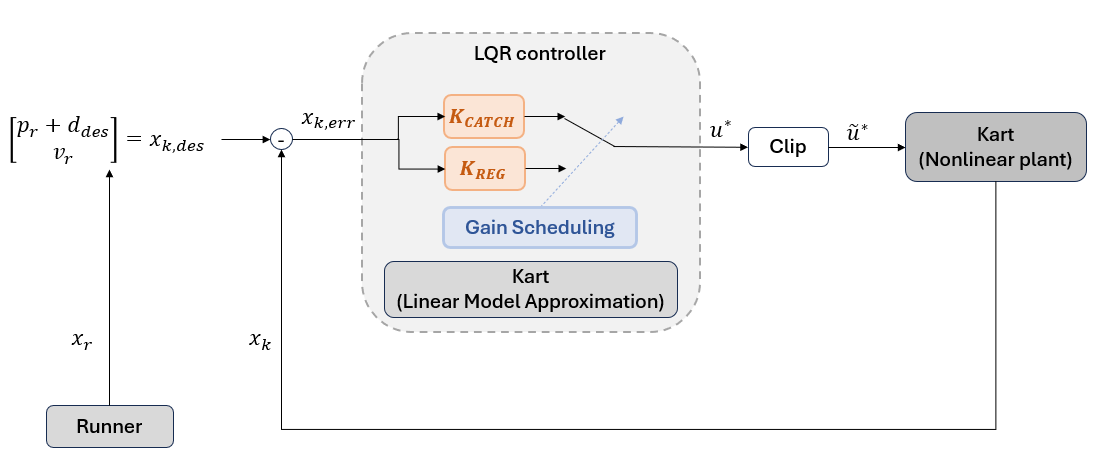
\includegraphics[width=1.0\textwidth]{LQR_sim_scheme.png}
	\caption{Linear Quadratic Regulator control scheme}
	\label{image:LQR_sim_scheme}
\end{figure}

The most challenging phase of the motion occurs in the first few seconds when the runner accelerates faster than the maximum acceleration the kart can achieve.
This phase, known as the 'catch-up maneuver', necessitates implementing a safety measure to prevent potential collisions between the airshield and the runner. 
Therefore, the runner begins the sprint from a position several meters farther from the kart than the steady-state desired distance $d_{\text{des}}$.

Hence, the initial condition for the kart state is set to be the following:
\begin{equation}
    x_{k,\text{init}} =
    \begin{bmatrix}
        d_{\text{des}} + \bar{d} \\
        0
    \end{bmatrix}
\end{equation}
where $\bar{d}$ is a parameter dependent on the runner's expected acceleration along the performance.
 

During the catch-up phase, the control action is governed by the controller gain $K_{\text{catch}}$ computed using the following weighting matrices:
\begin{equation}
    Q_{\text{catch}} =
    \begin{bmatrix}
        40 & 0 \\
        0 & 1000
    \end{bmatrix},
    \quad
    R_{\text{catch}} = [2]
\end{equation}

As evidenced by the weight selection, the primary objective during the catch-up maneuver is to match the go-kart velocity with that of the runner.
To facilitate this objective, a significantly higher weight is assigned to the second state variable.
This weights configuration enables the kart to start accelerating at its maximum capability, even if the runner remains at a distance greater than the desired value $d_{\text{des}}$.
Such an approach prevents unsafe scenarios where the runner's higher velocity could lead to a collision with the shield.

\subsection{Cruise maneuver}
Once the alignement between the kart and runner velocity is achieved, typically at an 80\% match, the controller switches to $K_{\text{cruise}}$.
This controller assigns nearly equal importance to distance and velocity mismatch.
While a preference for the velocity state persists, the significance given to the kart's position relative to the runner's is significantly increased.

The weight matrices for this cruise control configuration are as follows:
\begin{equation}
    Q_{\text{cruise}} =
    \begin{bmatrix}
        800 & 0 \\
        0 & 4000
    \end{bmatrix},
    \quad
    R_{\text{cruise}} = [0.002]
\end{equation}
This setup enables a rapid and substantial reduction in the relative distance to the desired value once the velocities of the go-kart and runner are already aligned.
Once the desired value $d_{\text{des}}$ is reached, the $K_{\text{cruise}}$ controller and its corresponding control law are able to maintain the system around the desired operating conditions.

\bigskip
The overall control scheme is illustrated in figure \ref{image:LQR_sim_scheme}, while algorithm \ref{alg:LQR_sim_implementation} outlines the steps followed by the LQR algorithm while controlling the system.

\begin{algorithm}
\begin{algorithmic}[1]
	\State catched = false;
	\State Set initial runner position with a proper distance $\bar{d}$ from kart;
	\For{$t=0,1,2,...$};
		\State Take kart state information $x_{k,t} = [p_{k,t}, v_{k,t}]^\top$;
		\State Take runner state information $x_{r,t} = [p_{r,t}, v_{r,t}]^\top$;
		\State Compute corresponding desired state for kart $x_{k,t,des} = [p_{r,t} + d_{\text{des}}, v_{r,t}]^\top$;
		\If{$v_{k,t} \geq 0.8 v_{r,t}$ \textbf{and} catched = false}
			\State catched = true;
		\EndIf
		\If{catched = false}
			\State $u^* = - K_{\text{catch}} (x_{k,t} - x_{k,t,des}) $;
		\Else 
			\State $u^* = - K_{\text{cruise}} (x_{k,t} - x_{k,t,des}) $;
		\EndIf
		\State Clip input according to limit saturation limits $\tilde{u}^* = \text{sat}_{[a_{\min}, a_{\max}]} (u^*)$;
		\State Inject $\tilde{u}^*$ in the plant;
	\EndFor
\caption{LQR implementation}
\label{alg:LQR_sim_implementation}
\end{algorithmic}
\end{algorithm}


\section{Model Predictive Control design}
The primary purpose of the Model Predictive Control scheme design lies in the possibility of including constraints, in the incorporation of a runner model within the predictive framework and in the simplification of the overall control architecture.
The gain scheduling approach, which switches between two controllers depending on the operational conditions, can be replaced with a single MPC controller.
Additionally, explicitly including constraints in the MPC formulation enables the encoding of safety guarantees within the control scheme. 
Examples of such constraints include maintaining a minimum safety distance or imposing bounds on maximum velocities to mitigate the risk of injuries.

\bigskip
Consider the linear model approximation \eqref{Linear_system} for the go-kart dynamics, and introduce the following integrator model for the runner, considered as an autonomous system:

\begin{equation}
\begin{cases}
	\begin{aligned}
		p_{r,t+1} &= p_{r,t} + dt \, v_{r,t} \\
		v_{r,t+1} &= v_{r,t} + dt \, a_{r,t}
	\end{aligned}
\end{cases}
\label{Runner_model}
\end{equation}
This model assumes constant acceleration for the runner, providing a simplified yet effective representation of his behavior.

Incorporating this assumption, we define the augmented state for the MPC prediction model as:
\begin{equation}
    x_p = 
    \begin{bmatrix}
        \Delta p  \\
        \Delta v \\
        v_k
    \end{bmatrix}
\end{equation}
where $\Delta p := p_k - p_r$ and $\Delta v := v_k - v_r$ represent the relative distance and velocity between the kart and the runner at a given time, respectively.

The overall prediction model, in discrete-time, state-space formulation can be written as follows:

\begin{equation}
\begin{aligned}
    x_{p,t+1} = 
        \begin{bmatrix}
            \Delta p_{t+1}  \\
            \Delta v_{t+1} \\
            v_{k,t+1}
        \end{bmatrix}
        & =
        \begin{bmatrix}
            1 & dt & 0 \\
            0 & 1 & -dt\frac{C_f}{m} \\
            0 & 0 & 1-dt\frac{C_f}{m}
        \end{bmatrix}
        x_{p,t}
        +
        \begin{bmatrix}
            0 \\
            dt \frac{C_{m1}}{m} \\
            dt \frac{C_{m1}}{m}
        \end{bmatrix}
        u_t + 
        \begin{bmatrix}
        0 \\
        - dt a_{r,t} \\
        0
        \end{bmatrix} \\
        & = A_p \, x_{p,t} + B_p \, u_t + a_t
\end{aligned}
\label{Prediction_model_MPC}
\end{equation}

where
\begin{equation}
    A_p =
        \begin{bmatrix}
            1 & dt & 0 \\
            0 & 1 & -dt\frac{C_f}{m} \\
            0 & 0 & 1-dt\frac{C_f}{m}
        \end{bmatrix}
    \quad
    B_e = 
        \begin{bmatrix}
            0 \\
            dt \frac{C_{m1}}{m} \\
            dt \frac{C_{m1}}{m}
        \end{bmatrix}.
\label{Prediction_matrices}
\end{equation}

The runner's actual acceleration $a_{r,t}$ is considered to be known and introduced in the prediction model as a linear affine term that allows the predictions to better fit with the real future runner behaviour.
This term, relative to the actual runner acceleration can be seen as the introduction of a known disturbance in the system, thus the term $a_t = [0, -dt a_{r,t}, 0]^\top$.

\bigskip
The optimal control problem solved at each discrete time instant, in a receiding horizon fashion, has the following formulation:
\begin{equation}
\begin{alignedat}{2}
	\min_{\substack{\boldsymbol{x}, \boldsymbol{u}}}\quad &\sum_{i=t}^{t+N-1} (x_{p,i|t} - x_{p,\text{des}}) ^\top \, Q \, (x_{p,i|t} - x_{p,\text{des}}) +  u_{i|t}^\top \, R \, u_{i|t} &&   \\
	\text{subj. to} & \quad x_{p,i+1|t}  = A_p \, x_{p,i|t} + B_p \, u_{i|t} + a_t  \hspace{1.5cm} t = 0, 1 \ldots N && \\
    &\quad a_{\text{min}} \leq u_{i|t} \leq a_{\text{max}}&& \\
    &\quad d_{\text{safe}}\leq \Delta p_{i|t} &&  \\
    &\quad x_{p,t|t} = x_{p,\text{meas}} &&
\end{alignedat}
\label{MPC_formulation}
\end{equation}
where the reference values for the prediction states are the following
\begin{equation}
    x_{p,\text{des}} =
    \begin{bmatrix}
        d_{\text{des}}  \\
        0 \\
        0
    \end{bmatrix}
\end{equation}
and $d_{\text{safe}}$ is a minimum distance between go-kart and runner, ensuring a safe situation.

\bigskip
The parameter $N$ defines the prediction horizon, representing the number of control intervals the controller must evaluate for prediction. 
Selecting this parameter requires careful consideration, as increasing the lenght of the prediction horizon also increases the complexity of solving the optimization problem.
This problem could have important consequences in systems having fast dynamics, where the number of prediction steps is limited by the processor power.
At the same time the prediction horizon has to be chosen long enought to adequately capture the system dynamics.
The optimal input sequence, obtained by repeatedly solving the optimizaton problem at each time step, is represented as $\boldsymbol{u}^* \in \mathbb{R}^{m \times N}$.

\bigskip
The weights in the cost function are less sensible to changes with respect to those used in the LQR formulation and are chosen as follows:
\begin{equation}
    Q =
    \begin{bmatrix}
        2.5 & 0 & 0 \\
        0 & 5 & 0 \\
        0 & 0 & 0
    \end{bmatrix},
    \quad
    R = [0.02]    
\end{equation}
The last element in the $Q$ matrix is chosen to be equal to zero since there is no reference for the absolute kart velocity.
Consequently, the third state is not taken into account in the cost function of the optimization problem.
However it is kept in the state vector because it makes possible to write the prediction model in an easier way.

\begin{figure}
	\centering
	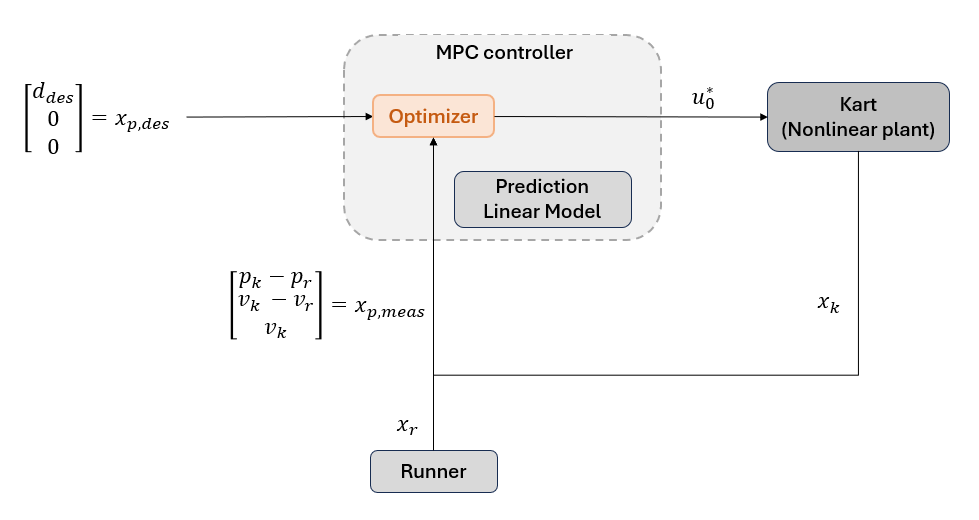
\includegraphics[width=1.0\textwidth]{MPC_sim_scheme.png}
	\caption{Model Predictive Control scheme}
	\label{image:MPC_sim_scheme}
\end{figure}

\begin{algorithm}
\begin{algorithmic}[1]
	\State Define desired prediction state $x_{p,\text{des}} = [d_{\text{des}}, 0, 0]^\top$;
	\State Set initial runner position with a proper distance $\bar{d}$ from kart;
	\For{$t=0,1,2,...$}
		\State Take prediction state information $x_{p,t} = [\Delta p_t, \Delta v_t, v_{k,t}]^\top$;
		\State Solve the constrained QP and get $\boldsymbol{u}^* = \{u_0, u_1, \cdots, u_N\}$; 
		\State Inject the first element of the optimal input sequence $u_0^*$ in the plant;
	\EndFor
\caption{MPC implementation}
\label{alg:MPC_sim_implementation}
\end{algorithmic}
\end{algorithm}
\bigskip
The overall MPC control scheme is shown in figure \ref{image:MPC_sim_scheme}, and it offers an important semplification in the architecture, with respect to the LQR case in figure \ref{image:LQR_sim_scheme}.
 Algorithm \ref{alg:MPC_sim_implementation} outlines the steps of the MPC implementation.

\section{Offset-free Model Predictive Control and Disturbance Observer design}
The MPC problem, as formulated in \eqref{MPC_formulation} employs as prediction model a linear affine approximation of the kart dynamics (see \eqref{Linear_system}), augmented with the runner model in \eqref{Runner_model}.
However, this prediction model does not take into account the nonlinear term arising from the drag coefficient present in the identified kart dynamic equations in \eqref{Plant_simplified}.
The true nonlinear prediction model for MPC, thus, should incorporate the additional nonlinear term, as in the following:

\begin{equation}
\begin{aligned}
    \begin{bmatrix}
        \Delta p_{t+1}  \\
        \Delta v_{t+1} \\
        v_{k,t+1}
    \end{bmatrix}
    & =
    \begin{bmatrix}
        1 & dt & 0 \\
        0 & 1 & -dt\frac{C_f}{m} \\
        0 & 0 & 1-dt\frac{C_f}{m}
    \end{bmatrix}
    x_{p,t}
    +
    \begin{bmatrix}
        0 \\
        dt \frac{C_{m1}}{m} \\
        dt \frac{C_{m1}}{m}
    \end{bmatrix}
    u_t + 
    \begin{bmatrix}
    0 \\
    - dt a_{r,t} \\
    0
    \end{bmatrix} 
    -
    \begin{bmatrix}
    0 \\
    dt (\frac{C_{d}}{m} v_{k,t}^2+ \frac{C_{roll}}{m}) \\
    dt (\frac{C_{d}}{m} v_{k,t}^2+ \frac{C_{roll}}{m})
    \end{bmatrix}
\end{aligned}
\label{Non-lin_prediction_model_MPC}
\end{equation}

where the last term includes the nonlinear and unmodelled drag effect, represented by the $w$ term in \eqref{Plant_model_mismatch},  signifying the model-plant mismatch within the offset-free MPC context.

\bigskip
Since MPC derives its solution based on the linear model in \eqref{Prediction_model_MPC}, the performance of the controller inherently depends on the magnitude of the unmodeled effects.
Therefore, achieving optimal closed-loop performance using the nominal MPC formulation may be challenging.
Offset-free MPC is designed to handle this kind of situations where there are discrepancies between the nominal model used for prediction and the actual plant dynamics. 

\bigskip
Data-driven control strategies, on the contrary, do not rely on models and can implicitly manage uncertainties in processes. 
However, pure data-driven approaches, without any prior assumption about the process, necessitate extensive data and typically employ slow exploratory techniques.
Recent control methodologies blend model-based techniques with data-driven approaches to overcome these limitations.
The reasoning used in this thesis to compensate for the model-plant mismatch term, combines a predictive control based on the linear prediction model with a real-time estimation and compensation of the nonlinear term based on data from the system.
This control strategy dynamically estimates discrepancies using the prediction errors, capturing the difference between the model's predictions and the actual system response.

Although offset-free MPC can mitigate model-plant mismatch, estimating in real-time the disturbances via an observer introduces a delay. 
This delay may result in disturbance compensation being optimal only at steady-state and not during transient phases when the disturbance varies.

\bigskip
Considering the problem statement presented in \eqref{MPC:offset-free}, the affine term that takes into account the runner acceleration, has been added, similar to the nominal MPC case.

The augmented prediction model in \eqref{Augmented_model}, necessary to the offset-free formulation is applied and it results to be:
\begin{equation}
\begin{aligned}
	x_{p,t+1} & = A_p \, x_{p,t} + B_p \, u_t + a_t + B_d \, d_t \\
    	d_{t+1} & = d_t
\end{aligned}
\label{Offset-free_prediction_model_MPC}
\end{equation}
where the matrices $A_p$, $B_p$ and the vector $a_t$ are defined in \eqref{Prediction_matrices} and $d_t$ is a scalar.

The term $B_d = [0, 1, 1]^\top$ signifies that the disturbance affects only in the second and third states, while the relative position prediction model remains unaffected by the mismatch with the plant.
For the purposes of this thesis the state is considered to be fully observable (i.e. $C = I_3$) and, as a consequence, the reference for the measured plant output is translated in reference for the plant states, thus $y_{\text{des}} = x_{p,\text{des}} = [d_{\text{des}}, 0, 0] ^\top$.
Accordingly also $C_d = [0, 0, 0]^\top$. 

\bigskip
The design of the observer plays a crucial role in enhancing the robustness of the proposed control scheme and it becomes:
\begin{equation}
    \begin{aligned}
    	\begin{bmatrix}
    	   \hat{x}_{p,t+1} \\
            \hat{d}_{t+1}
        \end{bmatrix}
	= A_e 
        \begin{bmatrix}
        \hat{x}_{p,t} \\
        \hat{d}_t
    	\end{bmatrix}
        + 
        B_e \, u +
        L (
         - x_{p,t} +
        C_e
        \begin{bmatrix}
            \hat{x}_{p,t} \\
            \hat{d}_t
        \end{bmatrix} )
    \end{aligned}
\end{equation}
where
\begin{equation}
    A_e =
    \begin{bmatrix}
        A_p & B_d \\
        0 & 1  
    \end{bmatrix},
    \quad
    B_e = 
    \begin{bmatrix}
        B_p \\
        0  
    \end{bmatrix},
    \quad
    C_e = 
    \begin{bmatrix}
        I_3 & 0 
    \end{bmatrix}.
\label{Observer_real}
\end{equation}

\bigskip
The observer gain matrix $L$ is designed in such a way the poles of $(A_e + L C_e)$ are placed in $\lambda=[0.5, 0.51, 0.52, 0.53]$, ensuring the resultant matrix to be Hurwitz. 
The same weighting matrices $Q$ and $R$ utilized in the nominal MPC context are employed as weights.

\bigskip
The final resulting offset-free formulation can be summarized in the following constrained optimization problem:
\begin{equation}
\begin{alignedat}{2}
	\min_{\substack{\boldsymbol{x}, \boldsymbol{u}}}\quad & \sum_{i=t}^{t+N-1} (x_{p,i|t} - \bar{x}_t) ^\top \, Q \, (x_{p,i|t} -  \bar{x}_t) +  (u_{i|t} - \bar{u}_t)^\top \, R \, (u_{i|t} - \bar{u}_t) &&  \\
	\text{subj. to} & \quad x_{p,i+1|t}  = A_p \, x_{p,i|t} + B_p \, u_{i|t} + a_t + B_d \, d_{i|t} \hspace{1.5cm} t = 0, 1 \ldots N &&  \\
    & \quad d_{i+1|t}  = d_{i|t} && \\
    &\quad a_{\text{min}} \leq u_{i|t} \leq a_{\text{max}}&& \\
    &\quad d_{\text{safe}}\leq \Delta p_{i|t} &&  \\
    &\quad x_{p,t|t} = \hat{x}_t && \\
    &\quad d_{t|t} = \hat{d}_t && 
\end{alignedat}
\label{MPC:offset-free}
\end{equation}
where $\bar{x}_t \in \mathbb{R}^n$ and $\bar{u}_t \in \mathbb{R}^m$ are solution of the following system:

\begin{equation}
    \begin{bmatrix}
    A_p-I_3 & B_p \\
    I_3 & 0
	\end{bmatrix}
 	\begin{bmatrix}
		\bar{x}_t \\
		\bar{u}_t
	\end{bmatrix}
    =
    \begin{bmatrix}
    -B_d \hat{d}_t\\
    x_{p,\text{des}} - C_d \hat{d}_t
	\end{bmatrix}
\end{equation}

\begin{figure}
	\centering
	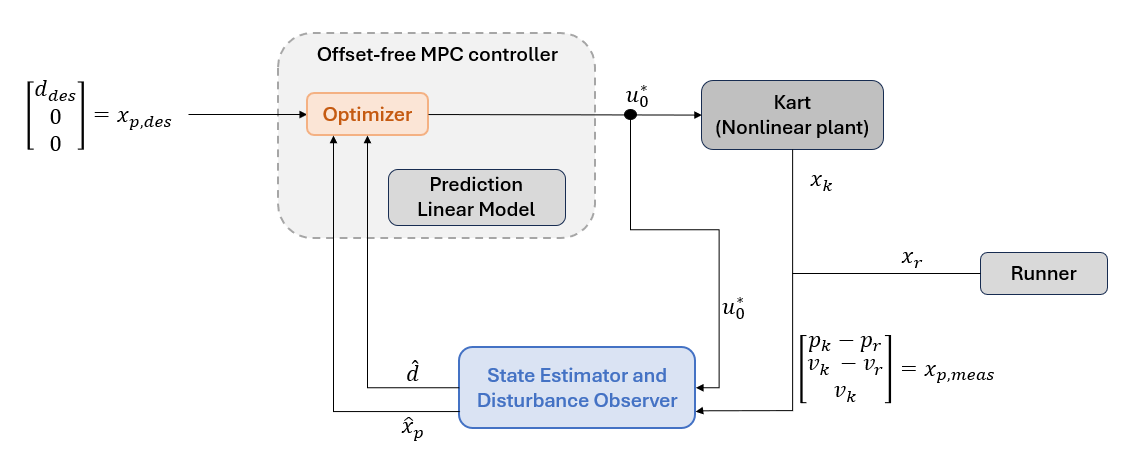
\includegraphics[width=1.0\textwidth]{MPC_of_scheme.png}
	\caption{Offset-free Model Predictive Control scheme with disturbance observer}
	\label{image:mpc_of_scheme}
\end{figure}

\begin{algorithm}
\begin{algorithmic}[1]
	\State Define desired prediction state $x_{p,\text{des}} = [d_{\text{des}}, 0, 0]^\top$;
	\State Set initial runner position with a proper distance $\bar{d}$ from kart;
	\State Initialize estimator $\hat{x}_{p,0} = [d_{\text{des}}, 0, 0]^\top$ and $\hat{d}_0 = 0$;
	\For{$t=0,1,2,... $}
		\State Take state estimator and disturbance observer information $\hat{x}_{p,t}$ and $\hat{d}_t$;
		\State Solve the constrained QP and get $\boldsymbol{u}^* = \{u_0, u_1, \cdots, u_N\}$; 
		\State Inject the first element of the optimal input sequence $u_0^*$ in the plant;
		\State Update state estimator and disturbance observer 
	\EndFor
\caption{MPC Offset-free implementation}
\label{alg:MPCOF_sim_implementation}
\end{algorithmic}
\end{algorithm}

\bigskip
In figure \ref{image:mpc_of_scheme} the block diagram of the proposed offset-free MPC with disturbance observer implementation is represented and algorithm \ref{alg:MPCOF_sim_implementation} describes the point of both estimation and control followed by the scheme.

\newpage
\section{Fluid-dynamic studies}

Fluid dynamics is a branch of physics that deals with the study of how fluids (liquids and gases) behave when they are in motion.
In the context of sports engineering, fluid dynamics plays a crucial role in understanding the interaction between athletes and the surrounding air or water during their performance.

Aerodynamics, a subfield of fluid dynamics, specifically focuses on the study of how moving objects interact with the air. 
The drag force, a key parameter in aerodynamics, quantifies the resistance encountered by an object as it moves through a fluid like the air. 
It can be expressed mathematically using the drag equation:
\begin{equation}
	F_d = \frac{1}{2} C_d \rho A \, v^2
\end{equation}
where $F_d$ is the drag force, $\rho$ is the density of the fluid (air in this case), $A$ is the frontal area of the object moving in the fluid, 
$v$ is the velocity of the object ad $C_d$ the drag coefficient.
One notable characteristic of drag force is its dependence on the square of the velocity $(v^2)$, indicating that the resistance experienced by the object increases exponentially with its speed. 

\bigskip
Recent fluid-dynamic studies and simulations, conducted using wind tunnels and advanced computational methods by \cite{Coni_article}, have investigated the impact of the aerodynamic shield on the variation of the aerodynamic force acting on a runner across speeds ranging from $5$ to $13$ meters per second.

\begin{figure}[h!]
	\centering
	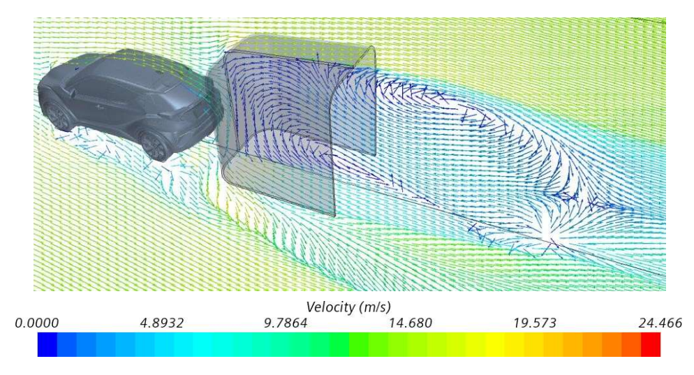
\includegraphics[width=0.7\textwidth]{Aerodynamics.png}
	\caption{}
	\label{image:Aerodynamic_studies}
\end{figure}

As depicted in figure \ref{image:Aerodynamic_studies}, when the air moves over the shield fails in following the curvature of the surface, and results to be reparated into two different flows.
This phenomenon is called flow separation.
This results in the formation of vortices and regions of recirculating flow, creating a significant low-pressure region behind the shield.
Interestingly, this aerodynamic configuration not only reduces air friction experienced by the athlete but also generates a pushing force from behind, aligning with the athlete's movement. 
Consequently, the athlete benefits from both a reduced air resistance and a propulsive force, potentially enhancing its speed and performance.

\bigskip
According to these results, the reference distance $d_{\text{des}}$ to be maintained between the runner and the kart can be assumed to be around $2.5$ meters, thus the athlete should be able to run on the airshield border or in the slipstream up to a couple of meters further.
In the following, for both the simulations and the real hardware tests, a $d_\text{des}$ of $2.5$ meters and $d_\text{safe}$ of $1.5$ meters are utilized.


\chapter{Numerical simulation results}
%\addcontentsline{toc}{chapter}{Simulations and Hardware results}
\markboth{}{SIMULATION RESULTS}
\label{chapter:Simulations_results}
The primary objective of this chapter is to present and analyze the results of Python simulations carried out on the nonlinear mathematical model of the go-kart with the airshield attached.
The simulations aim to mimic the behaviour of a runner during a competition or a training by utilizing a proper velocity profile.
The three controllers: Linear Quadratic Regulator, Model Predictive Control and Offset-Free Model Predictive Control have been tested and their performances are evaluated and compared.
Specifically, in section $3.1$, the data utilized for the controllers simulation tests are introduced.
It describes how they have been obtained from real competition results, together with a presentation of the parameters used for the comparison.
Section $3.2$ and $3.3$ are focused on finally evaluate and numerically compare the controllers performances in two distinct scenario.

\section{Test data and comparison parameters}
To assess the performance of the controllers and evaluate the application's behaviour, empirical data from two presigious Diamond League competitions \cite{diamondleague} have been employed, focusing on the winners of the 100 meters sprint event both in the man's and women's categories. 

\begin{table}[h!]
	\centering
	\begin{adjustbox}{max width=\textwidth}
	\begin{tabular}{c|c|c|c|c|c|c|c|c|c|c}
           & 10m & 20m & 30m & 40m & 50m & 60m & 70m & 80m & 90m &100m \\
	\hline
	\hline
	t & 1.97 & 3.10 & 4.11 & 5.08 & 6.03 & 6.99 & 7.94 & 8.90 & 9.88 & 10.88  \\	
	$\Delta t$ & 1.97 & 1.13 & 1.01 & 0.97 & 0.95 & 0.96 & 0.95 & 0.96 & 0.98 & 1.00 \\
	$\bar{v}_r$ & 5.07 & 8.85 & 9.90 & 10.31 & 10.53 & 10.42 & 10.53 & 10.42 & 10.20 & 10.00 \\
	\hline
	\end{tabular}
	\end{adjustbox}
\caption{Marie-Josèe Ta-Lou - Diamong League Lausanne 30th June 2023}
\label{tab:Women}
\end{table}

\bigskip
In the case of the women's 100m sprint event, data are taken from the competition held in Lausanne on June 30, 2023.  
The race saw Marie-Josèe Ta Lous as winner and in table \ref{tab:Women} are reported her timed intervals recorded at every 10 meters. 
Based on these splits an average velocity for each 10 meters interval has been computed in order to have a velocity runner profile over time.

\begin{table}[h!]
	\centering
	\begin{adjustbox}{max width=\textwidth}
	\begin{tabular}{c|c|c|c|c|c|c|c|c|c|c}
           & 10m & 20m & 30m & 40m & 50m & 60m & 70m & 80m & 90m &100m \\
	\hline
	\hline
	t & 1.87 & 2.89 & 3.80 & 4.67 & 5.52 & 6.36 & 7.21 & 8.07 & 8.93 & 9.83  \\	
	$\Delta t$ & 1.87 & 1.02 & 0.91 & 0.87 & 0.85 & 0.84 & 0.85 & 0.86 & 0.86 & 0.90 \\
	$\bar{v}_r$ & 5.35 & 9.80 & 10.99 & 11.49 & 11.76 & 11.90 & 11.76 & 11.63 & 11.63 & 11.11 \\
	\hline
	\end{tabular}
	\end{adjustbox}
\caption{Christian Coleman - Diamong League Eugene 16th September 2023}
\label{tab:Man}
\end{table}

Likewise, a similar methodology has been applied to the men's 100 meters competition, which took place in Eugen on September 16, 2023.
Christian Coleman clinched victory crossing the finish line in 9.83 seconds.
The detailed analysis of Coleman's performance and the corresponding average velocities derived from the intervals times are reported in table \ref{tab:Man}.

\begin{figure}[!h]
	\centering
	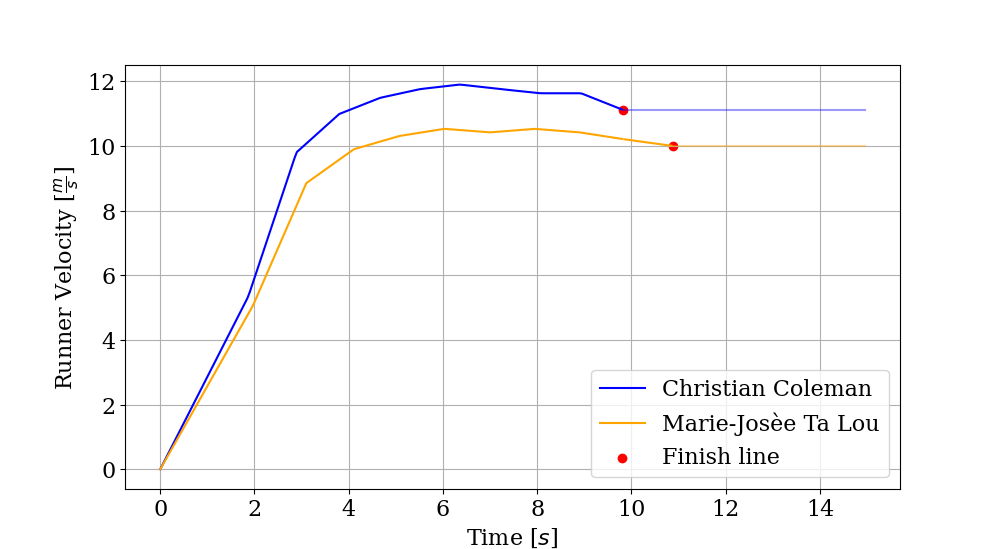
\includegraphics[width=0.7\textwidth]{Test_Velocities.png}
\caption{Velocities profiles used for simulation tests}
\label{Test_Velocities}
\end{figure}

The velocity profiles, obtained by interpolating the average velocities along time, are illustrated in figure \ref{Test_Velocities}.
The red dot denotes the moment when runners cross the finish line.
Subsequent to this event, the velocities are assumed to remain constant until a simulation time of $15$ seconds with the purpose of allowing for an evaluation of the controllers' steady-state performance.

\bigskip
The parameters used for the evaluation and comparison of the controllers' performances are the following:
\begin{itemize}
	\item Mean error (position and velocity): represents the average difference between the desired reference value and the actual plant output over the simulation period. It provides a measure of the overall accuracy of the controller's tracking performance.
	\item Integral Absolute Error (position and velocity): measures the cumulative sum of the absolute errors between the desired reference value and the actual plant output. It provides insight into the total deviation od the system's response from the desired trajectory.
	\item Minimum distance from kart: the concept is similar to the undershoot, thus it quantifies the extent to which the system's response deviates from the desired trajectory. This parameter quantifies how close the runner goes to the kart during the performance.
	\item Energy consumption: quantifies the amount of energy expended by the system to achieve the desired tracking performance.
	\item Stead-state error: characterizes the residual errror between the actual output and the desired reference value once the system has reached a stable operating condition, with the kart tracking a constant velocity of the runner.
	\item "Rise" time to reach the desired reference distance $d_\text{des}$: refers to the duration taken by the system's output to transition from the initial state to the desired position setpoint. It represents the speed at which the system responds to changes in the reference signal and it is indicative of the controller's dynamic responsiveness.
\end{itemize}

\subsection*{CVXPY and OSQP solver}
The quadratic optimization problems in the Model Predictive Control (MPC) formulations have been tackled using the CVXPY library \cite{diamond2016cvxpy}, a mathematical framework for solving optimization problems, along with the OSQP solver \cite{Stellato_2020}.
CVXPY facilitates the expression of convex optimization problems in a natural syntax that follows the mathematical formulations, which are then automatically converted into the standard form required by various solvers.
OSQP (Operator Splitting Quadratic Program) is a high-performance solver specifically designed for convex quadratic programming problems, making it particularly suitable for applications in control systems, robotics, and machine learning.

\section{Test on women velocity profile of Ta Lou}
\begin{figure}[h!]
    \centering
    \begin{subfigure}[t]{0.8\textwidth}
        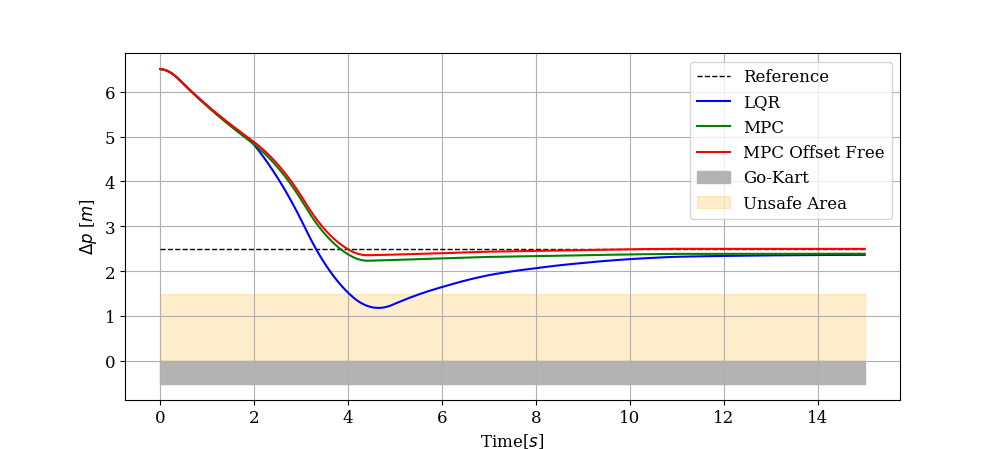
\includegraphics[width=\textwidth]{Ta_Lou/Deltap.png}
        \caption{Relative position between runner and go-kart}
        \label{fig:Deltapwomen}
    \end{subfigure}
    
    \begin{subfigure}[t]{0.8\textwidth}
        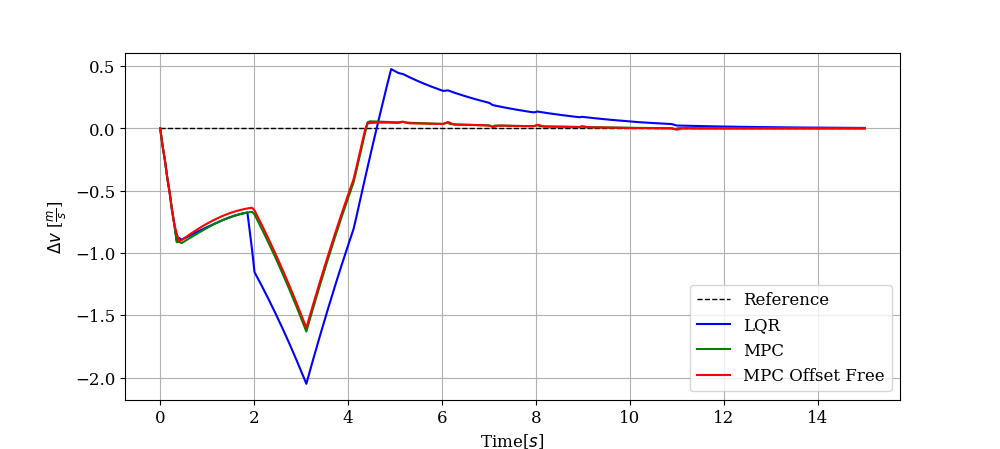
\includegraphics[width=\textwidth]{Ta_Lou/Deltav.png}
        \caption{Relative velocity between runner and go-kart}
        \label{fig:Deltavwomen}
    \end{subfigure}
    
    \begin{subfigure}[t]{0.8\textwidth}
        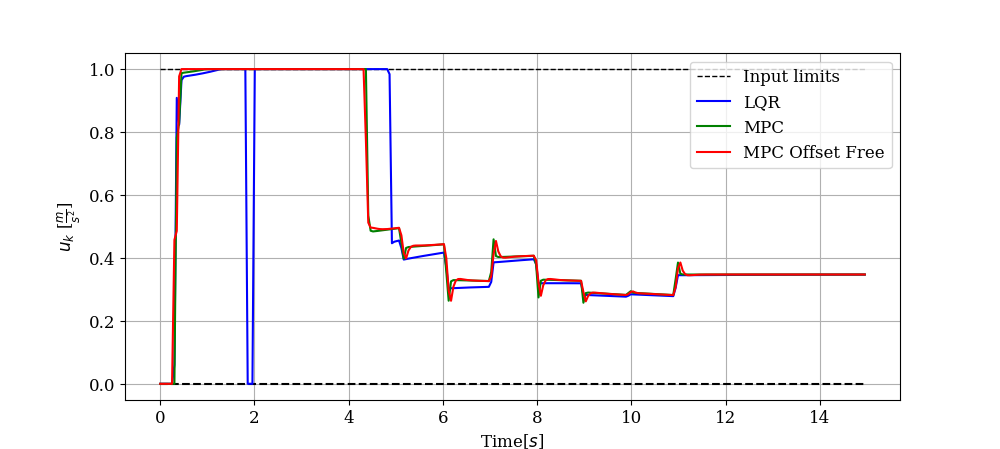
\includegraphics[width=\textwidth]{Ta_Lou/Input.png}
        \caption{Input effort (drive-train acceleration)}
        \label{fig:Inputwomen}
    \end{subfigure}
    \caption{Simulation results following Ta Lou velocity profile. The results for LQR (in blue), MPC (in green) and Offset-free MPC (in red) are shown overlapped on the same plot to appreciate the comparison among controllers}
    \label{fig:Women}
\end{figure}

The initial distance used for the simulation is $\bar{d} = 4$ meters.

\bigskip
Both Table \ref{tab:Ta_Lou} and figure \ref{fig:Women} clearly demonstrate that the LQR controller exibits poorer performance compared to the other controllers.
Specifically, considering the minimum distance between runner and go-kart, the LQR performs significantly worse than the other two controllers and violates the safety distance state constraints $d_{\text{safe}}$ introduced in both the MPC formulations.
Graphically, the region between the $d_\text{safe}$ and the airshield border is indicated in figure \ref{fig:Deltapwomen} with a yellow area.
This on represents an unsafe region for the controller to operate, since the distance between the runner and the go-kart to too small to guarantee a safety condition. 
The border of the airshield, thus the point where it is attached to the go-kart itself, is represented by the grey area.

The LQR has also the highest mean values of position deviation ($\Delta p$) and velocity deviation ($\Delta v$), indicating a less accurate tracking performance compared to MPC and MPC Offset-free.
Additionally, the fact that also the Integral of Absolute Error (IAE) metrics for both position and velocity are higher, suggests poorer tracking accuracy over the entire simulation period.
It's noteworthy that the offset-free version of the predictive controller achieves an almost zero steady-state error, significantly smaller than the approximately 10-centimeters values obtained with the other controllers. 
The three controllers show similar energy consumption over time.

\begin{table}[htbp]
	\centering
	\begin{tabular}{c|c|c|c}
          & \textbf{LQR} & \textbf{MPC} & \textbf{MPC Offset-free} \\
	\hline
	\hline
	mean($\Delta p$) & 0.8892 & 0.6867 &  0.6168 \\
	mean($\Delta v$) & 0.3987 & 0.2611 & 0.2522 \\
	IAE on $\Delta p$ & 13.2352 & 10.1978 & 9.1515 \\
	IAE on $\Delta v$ & 5.9811 & 3.9176 & 3.7826 \\
	min($\Delta p$) & 1.1885 & 2.2371 & 2.3605 \\
	Energy consumption & 0.5208 & 0.5200 & 0.5207 \\
	Steady state error & 0.1354 & 0.1079 & 0.0009 \\
	"Rise" time to $d_\text{des}$ & 3.3 & 3.75 & 3.85 \\
	\hline
	\end{tabular}
\caption{Comparison of controllers performance: Ta Lou velocity profile }
\label{tab:Ta_Lou}
\end{table}


\section{Test on men velocity profile of Coleman}
\begin{figure}[h!]
    \centering
    \begin{subfigure}[t]{0.8\textwidth}
        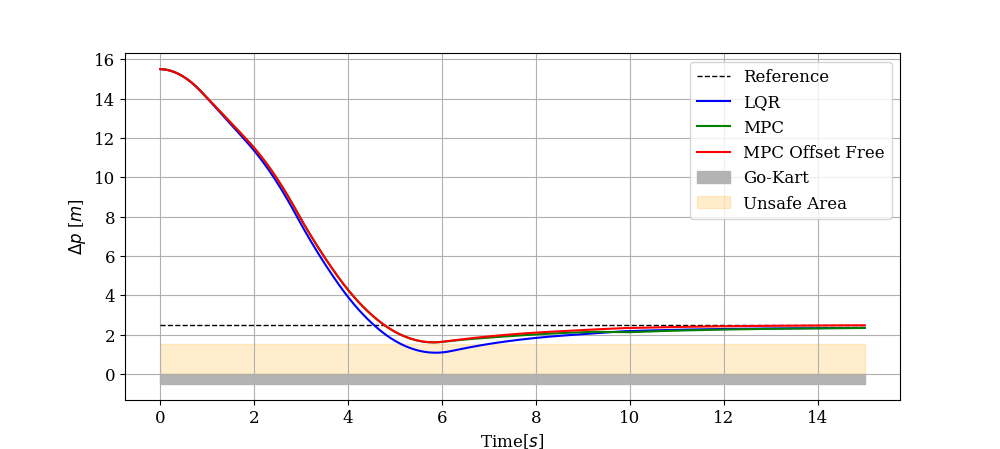
\includegraphics[width=\textwidth]{Coleman/Deltap.png}
        \caption{Relative position between runner and go-kart}
        \label{fig:Deltapmen}
    \end{subfigure}
    
    \begin{subfigure}[t]{0.8\textwidth}
        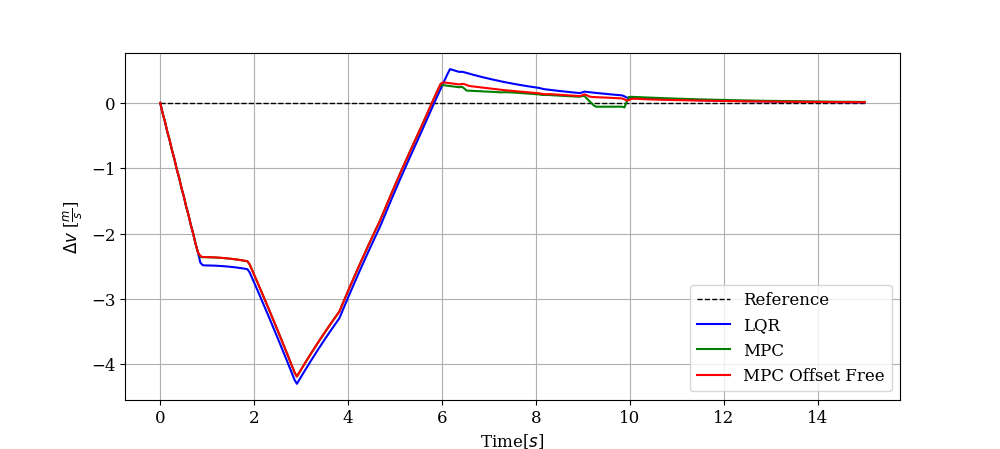
\includegraphics[width=\textwidth]{Coleman/Deltav.png}
        \caption{Relative velocity between runner and go-kart}
        \label{fig:Deltaven}
    \end{subfigure}
    
    \begin{subfigure}[t]{0.8\textwidth}
        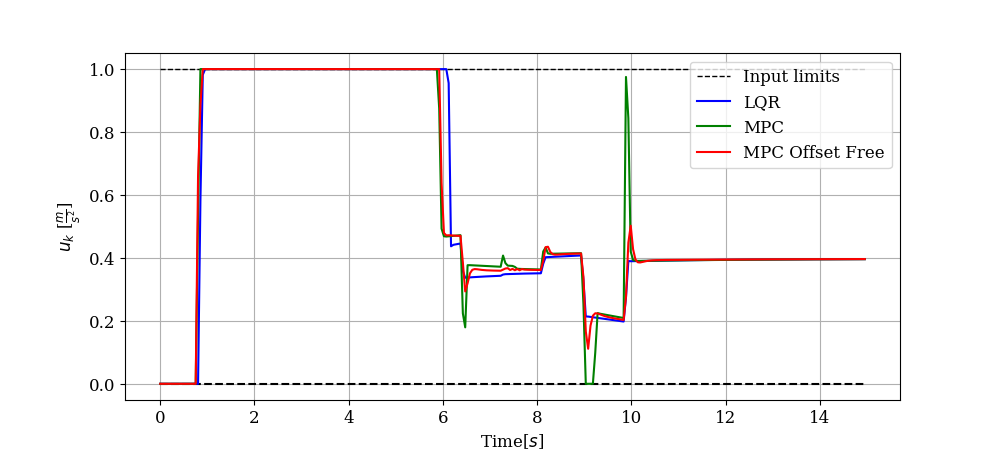
\includegraphics[width=\textwidth]{Coleman/Input.png}
        \caption{Input effort (drive-train acceleration)}
        \label{fig:Inputmen}
    \end{subfigure}
    \caption{Simulation results following Coleman velocity profile. The results for LQR (in blue), MPC (in green) and Offset-free MPC (in red) are shown overlapped on the same plot to appreciate the comparison among controllers}
    \label{fig:Men}
\end{figure}

It is reasonable that by intensifying the difficulty of the velocity profile from the one of a female runner to the one of male, the required initial distance from the go-kart is going to increase.
In the case of the Christian Coleman velocity profile this value is set to $\bar{d} = 13$ meters.

\begin{table}[h!]
	\centering
	\begin{tabular}{c|c|c|c}
          & \textbf{LQR} & \textbf{MPC} & \textbf{MPC Offset-free} \\
	\hline
	\hline
	mean($\Delta p$) & 2.5984 & 2.5636 &  2.4848 \\
	mean($\Delta v$) & 1.0037 & 0.9392 & 0.9419 \\
	IAE on $\Delta p$ & 38.6465 & 38.1247 & 36.9459 \\
	IAE on $\Delta v$ & 15.0578 & 14.0901 & 14.1308 \\
	min($\Delta p$) & 1.0802 & 1.6036 & 1.6105 \\
	Energy consumption & 0.5694 & 0.5694 & 0.5697 \\
	Steady state error & 0.1689 & 0.1784 & 0.0350 \\
	"Rise" time to $d_\text{des}$ & 4.5 & 4.7 & 4.7 \\
	\hline
	\end{tabular}
\caption{Comparison of controllers performance: Coleman velocity profile}
\label{tab:Coleman}
\end{table}

When intializing the maneuver from a further distance compared to the previous scenario, higher values of mean position error and Integral Absolute Error are observed, as reported in table \ref{tab:Coleman}.
The performance of the controllers can be graphically observed in figure \ref{fig:Men}.
The value of the minimum distance reached between the runner and the go-kart is much smaller for the LQR with respect to the two MPC formulations also in this simulation, indicating that the athlete enters a larger distance inside the shield. 
The recorded LQR value of 1 meter and 8 centimeters violates the safety bound introduced in the MPC, similar to the observation made in the Ta Lou velocity profile case.
Furthermore, it's worth noting that the offset-free MPC consistently outperforms both LQR and MPC in terms of steady-state error, achieving the lowest value among the three controllers.

It should be noticed that, in both the scenario saturation phenomenon is present for a consistent part of the tracking with the LQR controller.
Unlike MPC, which respects actuator limits, the LQR controller exhibits saturation, meaning that the control inputs are constrained to their maximum or minimum values for extended periods. 
This can lead to suboptimal performance.

\section{Disturbance observer results}

\begin{figure}[h!]
    \centering
    \begin{subfigure}[b]{0.49\textwidth}
        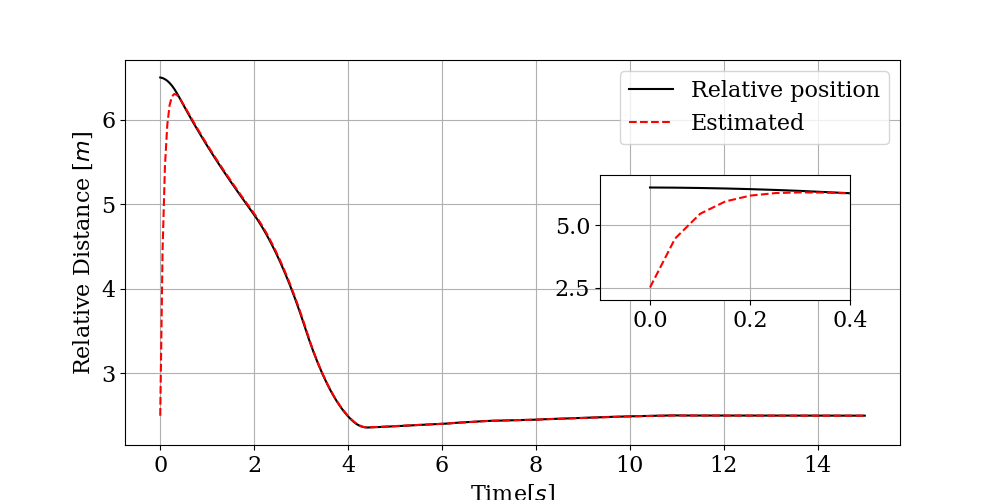
\includegraphics[width=\textwidth]{Estimator/Deltap.png}
    \caption{Relative position}
    \label{state1}
    \end{subfigure}
    \hfill
    \begin{subfigure}[b]{0.49\textwidth}
        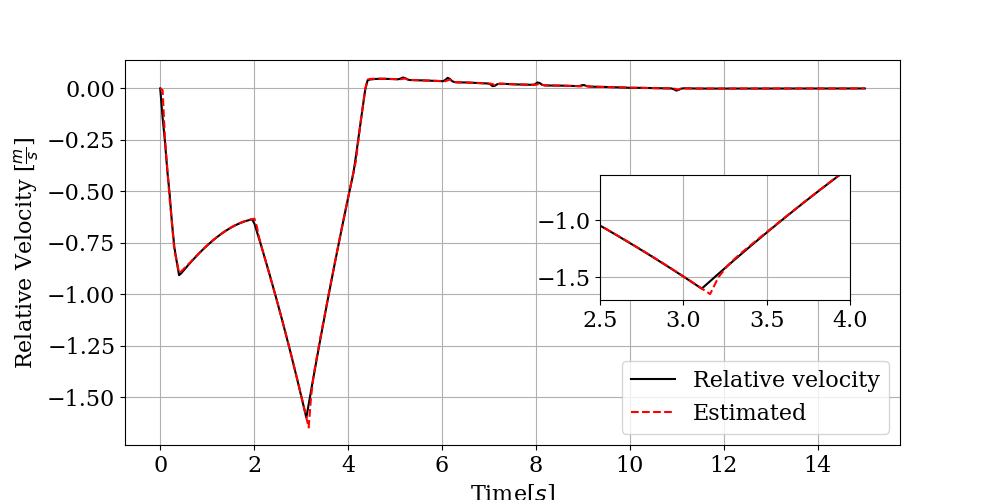
\includegraphics[width=\textwidth]{Estimator/Deltav.png}
    \caption{Relative velocity}
    \end{subfigure}
    \\[0.2cm]
    \begin{subfigure}[b]{0.49\textwidth}
        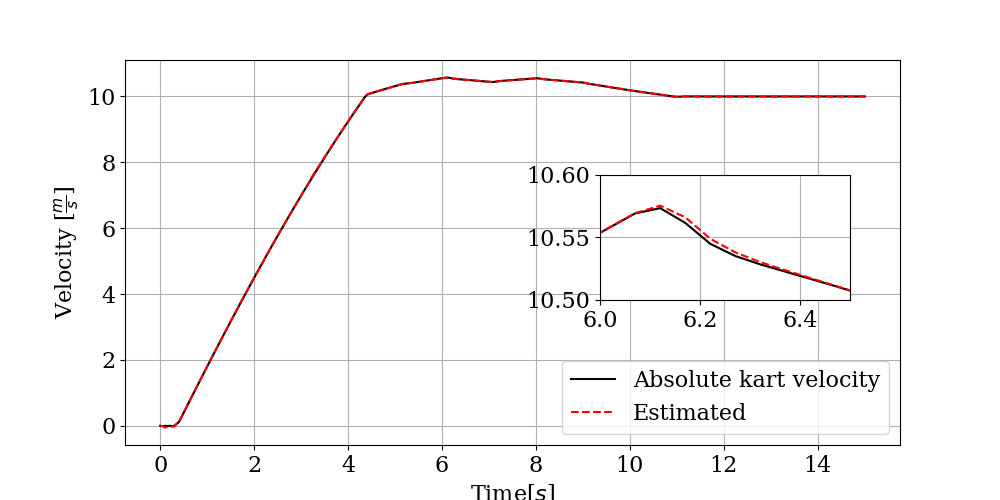
\includegraphics[width=\textwidth]{Estimator/vk.png}
    \caption{Absolute go-kart velocity}
    \end{subfigure}
    \hfill
    \begin{subfigure}[b]{0.49\textwidth}
        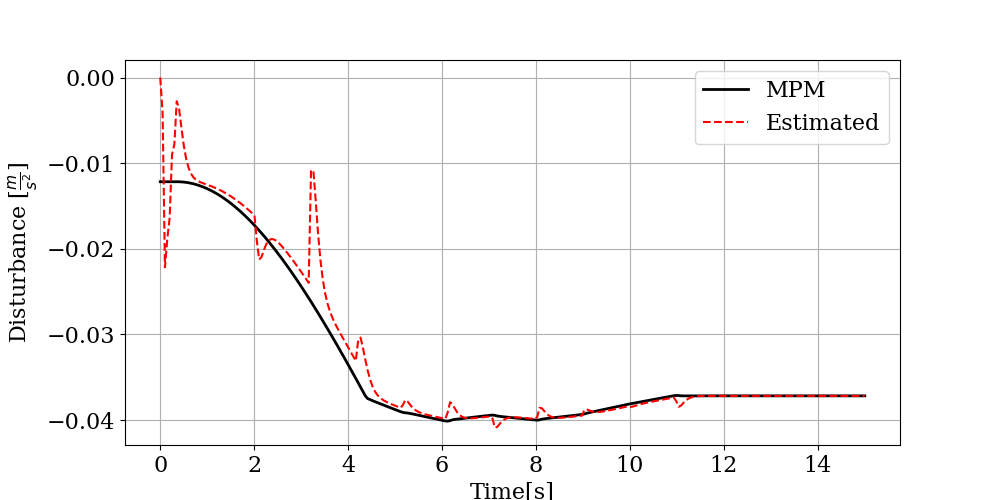
\includegraphics[width=\textwidth]{Estimator/mpm.png}
    \caption{Disturbance (model-plant mismatch}
    \label{disturbance}
    \end{subfigure}
    \caption{Estimated state variables (dashed red line) and observed model-plant mismatch term (dashed red line), compared to actual known values (black line)}
\label{Estimator}
\end{figure}

In this section, the output of the disturbance observer and state estimator, formulated in the state-space model in \eqref{Observer_real}, are presented.
The observer has the capability to simultaneously estimate the states and the unknown disturbance, representing the model-plant mismatch.

Figure \ref{Estimator} shows the three estimated state variables alongside their actual values in the case of Ta Lou simulation.
It is important to notice the ability and precision of the estimator in producing estimated values with only minor differences with respect to the actual ones.
Only minor delays, as highlighted in the subplot insets, are present when fast changes in the actual state variables occur.
These delays stem from the Luenberger observer's mechanism, which updates the estimated state variables based on the prediction error.

Focusing on subfigure \ref{state1}, the initial value for the estimator was set to $d_\text{des}$ without considering the $\bar{d}$ component relative and specific to the runner's acceleration intensity. 
However, the estimator quickly converges to the actual value and compensates for the incorrect initialization. 
This rapid adjustment is facilitated by selecting appropriate observer gain matrices, enabling the observer dynamical system in \eqref{Observer_real} to have a proper trade-off between responsiveness and accuracy in estimation.

In figure \ref{disturbance}, the observed disturbance is illustrated. 
This estimated disturbance captures the model-plant mismatch between the nonlinear kart plant model and the linear prediction model utilized for system control, as outlined in \eqref{Non-lin_prediction_model_MPC}.
This term represents the component related to the drag effect in the go-kart dynamics.
Furthermore, the magnitude of the estimated disturbance tends to be higher when the absolute velocity of the go-kart is elevated, gradually reaching a constant steady-state value as the system stabilizes.

The effectiveness of the disturbance observer in capturing the model-plant mismatch term is crucial, especially in the context of implementing offset-free Model Predictive Control. 
By accurately estimating both the state variables and the disturbance, the system can effectively compensate for discrepancies between the actual plant behavior and the model predictions, ultimately enhancing control performance.

 \chapter{Go-kart and Airshield Structure and Hardware-in-the-loop implementation}
\markboth{}{HARDWARE TEST RESULTS}
In this chapter an overview of the hardware structure and sensors equipment of the system is provided together with the changes in the controllers formulations with respect to the simulation environment. 
Later, an overview of the technologies studied and used for the implementation on the hardware of the control algorithms.
Finally, some test developed on the real hardware are presented and their results are shown and analyzed.

\section{System structure}

The system comprises a fully electric-powered go-kart with an attached airshield structure via a fixed joint. 
According to the CIK-FIA (International Karting Commission Federation International Automobile), a go-kart is a single-seater land vehicle with four non-aligned wheels in contact with the ground, two of which control steering while the others transmit power. 
Go-karts emerged after the post-war period of the 1950s, originally created by airmen as a pastime.
Typically, go-kart chassis are constructed from steel pipes that provide both stiffness and flexibility to compensate for the lack of a suspension system and a differential.

\subsection*{Electric-powered go-kart}
The kart is a SinusIon purchased from the German company RiMO (originally Richter + Mohn). 

\bigskip
The onboard battery is a lithium-iron-manganese-4-phosphate (LiFeMnPO4), used in order to reduce the battery pack weight.

\bigskip
For what regards the motor it is a Heinzmann PMS 100, with air-cooled cooling technology. 
This DC motor is a permanent magnet brushless motor with a link voltage of 28V, a nominal speed of 6500 rpm and a rated torque of 3.82 Nm, representing respectively the rotational speed at which the motor is designed to operate optimally and the maximum rotational force that the motor can exert.
In terms of efficiency, this motor is characterized with high efficiency and energy-saving capabilities, with a rated power output of 2.6kW. 
This parameter reflects the motor's ability to convert electrical energy into mechanical power.
The gearbox has a gear ratio of 1:7.

\bigskip
The computer on board is a AMD Ryzen MinisForum EliteMini X500 with an AMD Ryzen 7 5700G processor (8 cores with nominal frequency of 3.8GHz) coupled with a 16GB DDR4 RAM.

\subsection*{Airshield}

\begin{figure}
	\centering
	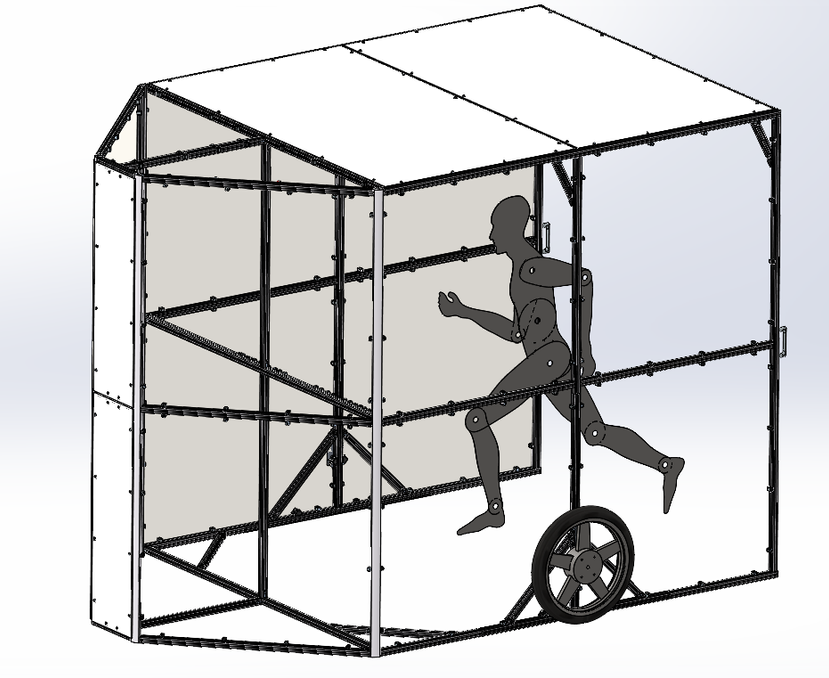
\includegraphics[width=0.5\textwidth]{Shield_structure.png}
\caption{Airshield structure}
\label{Shield_structure}
\end{figure}

The shield has the structure shown in \ref{Shield_structure}.
All the side and front panels are made of plexiglass while the top part is an aluminium composite.

The dimensions are reported in table \ref{tab:Shield_dimensions}.

\begin{table}[h]
\centering
\begin{tabular}{|p{1.5cm}|p{1.5cm}|p{1.5cm}|}
\hline
Height & 2.15 m \\
\hline
Width & 1.86 m \\
\hline
Lenght & 2.95 m \\
\hline
\end{tabular}
\caption{Aishield dimensions}
\label{tab:Shield_dimensions}
\end{table}
The height can be adjusted within a range of approximately $13$ centimeters by simply moving a wheel bracket up or down, in order to better fit the height of the runner.

\section{Perception}
Autonomous vehicles sense and perceive the surrounding environment using measurements coming from sensors and then process the information in order to make informed decisions. 
This is the fundamental principle behind closed-loop control that relies on measurements of controlled variables provided by an appropriate sensor.
The perception systems used in autonomous vehicles are usually categorized in two groups:
\begin{itemize}
    \item Proprioceptive sensors (or internal state sensors) sensing the vehicle's own state, like wheel encoders or inertial measurement unit, as well as location sensors like GPS, etc.
    \item Exteroceptive sensors (or external state sensors) gathering informations about the surrounding environment like cameras, LiDAR, RADARs, etc.
\end{itemize}
In this application the system is equipped with a LiDAR (Light Detection and Ranging), a camera, an inertial measurement unit and wheel encoders.

\subsection*{LiDAR}
LiDAR (Light Detected and Ranging) is a remote sensing technology that measures distances to objects and surfaces using laser pulses. 
The sensor consists of three main components: a laser emitter, a scanning mechanism, and a receiver.
The laser emitter sends out short pulses of laser light, which travel towards surrounding objects. 
When these pulses encounter an object, they reflect off its surface and return to the LiDAR sensor.
The receiver than detects the reflected light and measures the time it takes for the pulses to return, allowing the calculation of the distance to the object based on the speed of light.
Moreover, LiDAR rensors are capable of operating in various environmental conditions including darkness, rain, fow or low visibility, making them perfect for the application and highly reliable.

The LiDAR mounted on the airshield is a Velodyne VLP-16, a compact sensor that features 16 laser channels arranged in a circular configuration to have an important field of view.

The field of view (angular extension of a scene that is projected by the laser beam) is of 360$^\circ$ horizontal and 30$^\circ$ vertical.
The range of the laser is up to 100 meters. 
Measurements have an accuracy of +/- 3 cm and are acquired with a frequency of 20 Hz.

\subsection*{Camera}
Cameras provide rich information about the surrounding environment and can be used in a variety of ways.
On the airshield, a ZED 2i Stereo Camera with polarized lens of 4 millimeters is mounted.

The field of view is of 120$^\circ$ and the camera is able to sense ranges between 1.5 meters and 35 meters. 
The depth accuracy is smaller of the 2\% of the distance up to 10 meters while it increases up to the 7\% for distances up to 30 meters distance.

The camera is equipped with a Stereolab ZED Box Xavier NX 8GB, an industrial compact and powerful mini PC used for computing and processing camera data.
It's powered with an NVIDIA Jetson embedded GPU.

At the moment LiDAR measurements are prefered with respect to camera ones thanks to the higher accuracy.

\begin{figure}[h!]
	\centering
	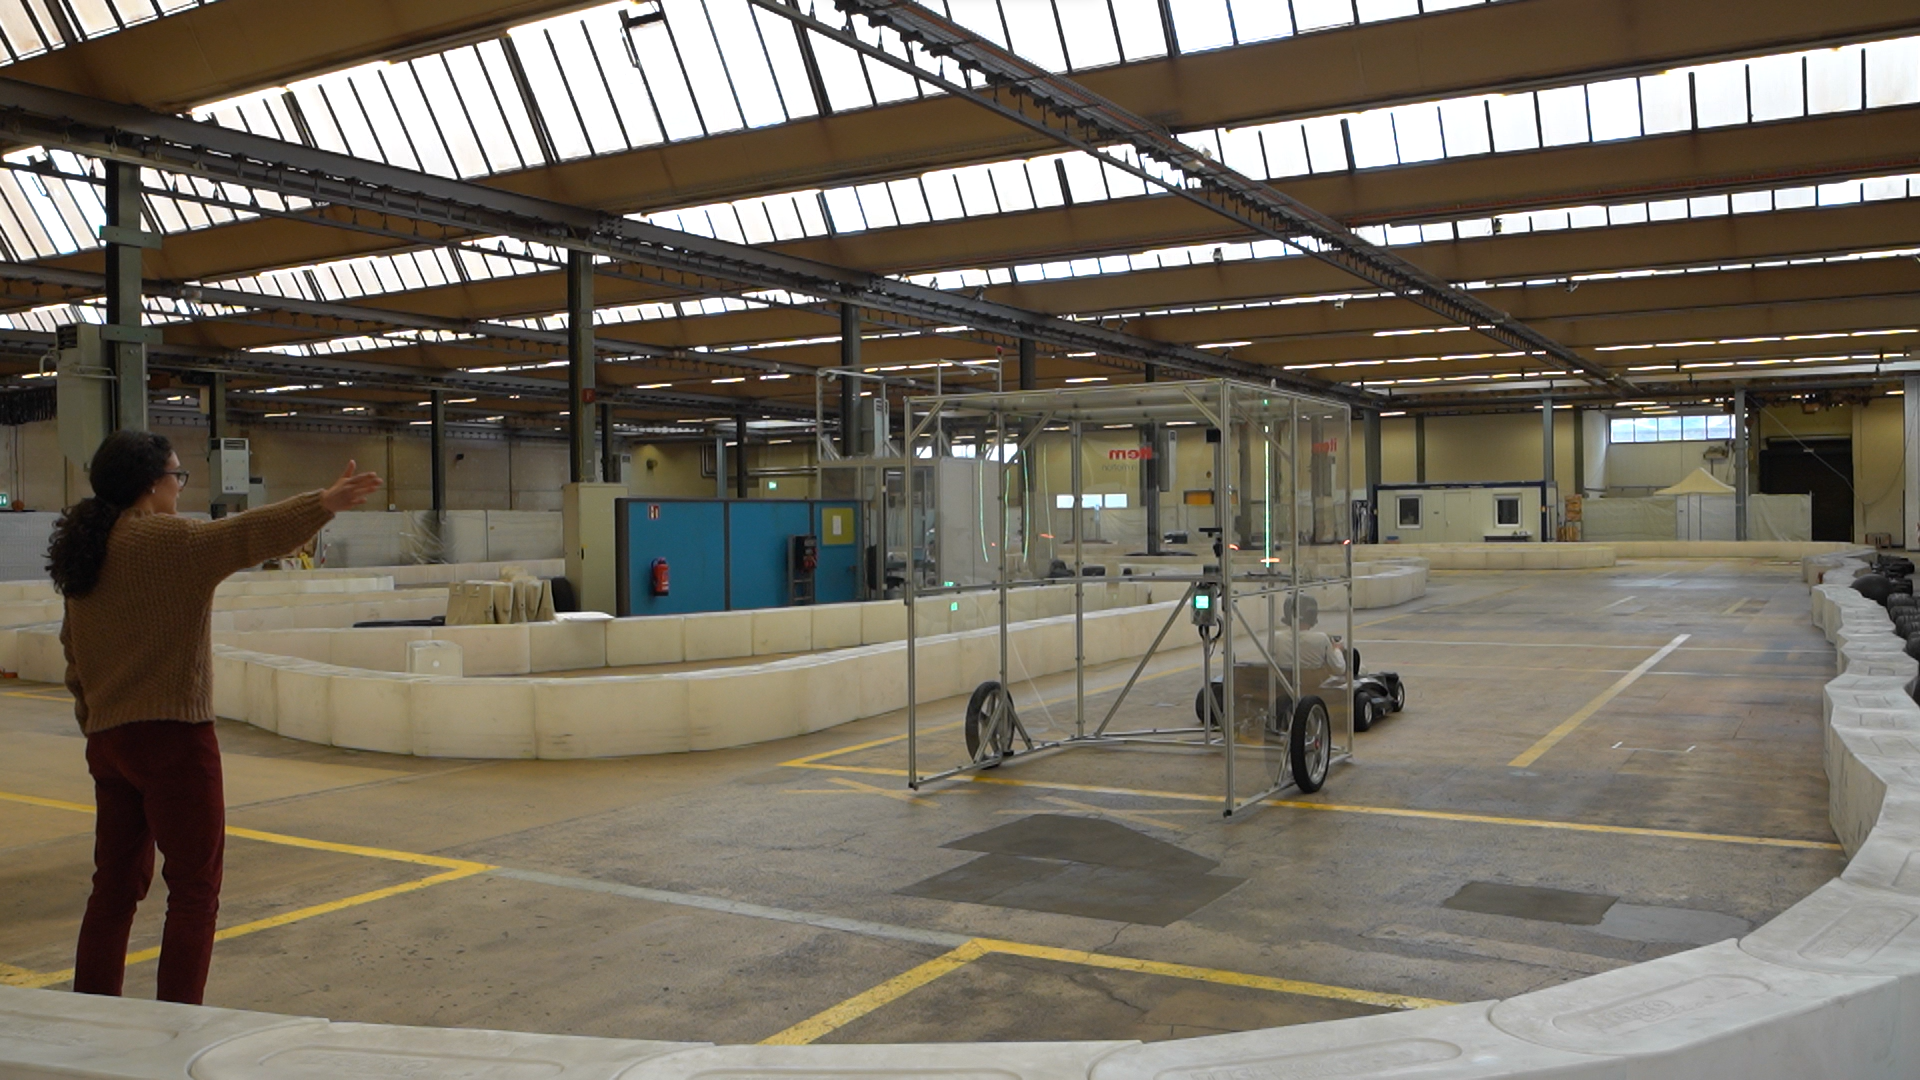
\includegraphics[width=0.5\textwidth]{Gesture.png}
\caption{Gesture used to activate the automatic controller ones the runner is ready to start the sprint}
\label{gesture}
\end{figure}

Camera remains responsible for the detection of the gesture to identify the moment in which the runner is able to start the performance. 
The recognition of this gesture, in figure \ref{gesture}, produces the activation of the automatic controller for the system.


\subsection*{Wheel Encoder}
Rotary encoders are a type of sensor that measure the rotation of a mechanical shaft.
Two wheel encoders, one for each wheel, are integrated in the PMS 100 motor as speed sensors, providing the motor's rotational speed.
Then, by knowing that the gear ratio is 1:7 and that the wheel diameter is $27.89$ centimeters the absolute go-kart speed can be evaluated using the following formula:

\begin{equation}
    v_{\text{kart}} = \frac{\pi \cdot d \cdot \text{avg rate}}{60 \cdot \text{gear ratio}}
\end{equation}
where avg rate is the average motor rate between left and right sides.



\subsection*{Inertial Measurement Unit}

\begin{figure}[h!]
	\centering
	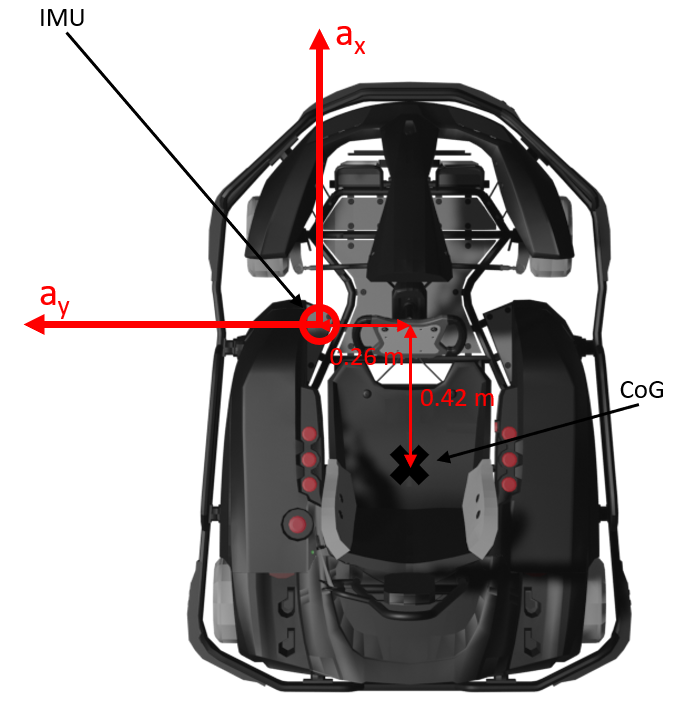
\includegraphics[width=0.3\textwidth]{IMU.png}
\caption{IMU position on the go-kart}
\label{IMU_pose}
\end{figure}

Typically an IMU or Inertial Measurement Unit consists of a combination of accelerometers and a gyroscopes, and sometimes also magnetometers in order to measure the orientation, velocity and acceleration of an object.
Thanks to the combination of accelerometers and gycopes, the IMU is able to sense the object's orientation or angular motion and acceleration with respect to some predefined axes.
The IMU used in the go-kart is the IRIMU-V2 from Izze-Racing that outputs data at 200Hz via CAN protocol and has an accuracy of less than 1\% of full scale for the acceleration and less than 1.5\% for the angular acceleration.
The position with respect to the go-kart centre of gravity is showed in \ref{IMU_pose}.

\newpage
\section{Controller design changes for hardware integration}
In the context of the control implementation for the hardware-in-the-loop tests, the available informations are the one coming from sensors and it is not possible to rely on a full state knowledge for both runner and kart as hypotized in Chapter 2.
For this reason it is important to take into account the sensors present in the system and the measurements provided by them to control the system properly. 
The changes occurred in the Linear Quadratic Regulator and in the nominal Model Predictive Control case are considered.

\subsection*{LQR}
Differently from the simulation context, where all the state variables both for runner and kart have been considered to be fully known, in the hardware-in-the-loop context, absolute position of both kart and runner, as well as the runner absolute velocity, result to be unknown.

\begin{figure} [h!]
	\centering
	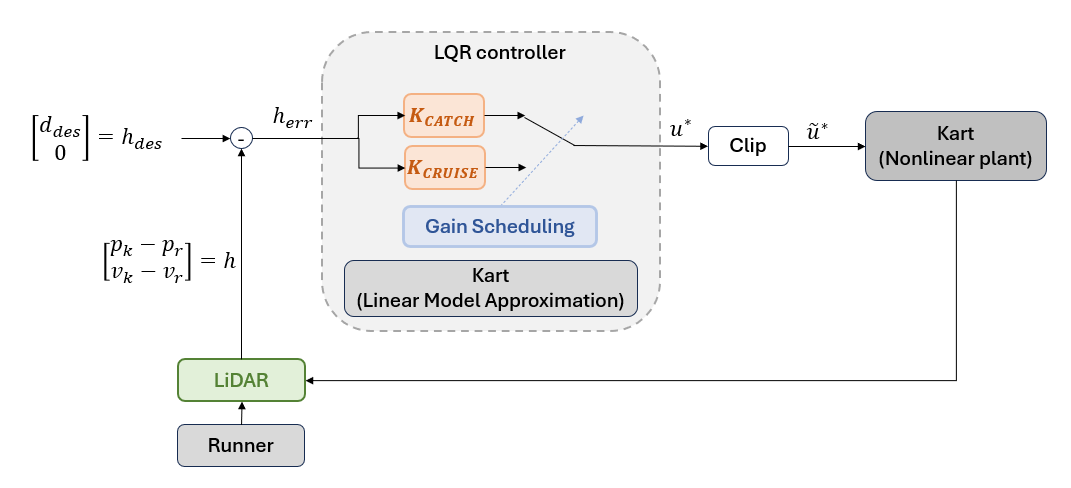
\includegraphics[width=1.0\textwidth]{LQR_hard_scheme.png}
	\caption{Linear Quadratic Regulator scheme with sensors}
	\label{image:LQR_hard_scheme}
\end{figure}

The LiDAR, as a range sensor, provides directly the measurement of the relative distance between runner and kart $\Delta p$, while the relative velocity can be estimated via finite differences:

\begin{equation}
	\Delta v_t = \frac{\Delta p_t - \Delta p_{t-1}} {dt}
\end{equation}
where $\Delta p_t := p_{k,t} - p_{r,t}$ and $\Delta v_t := v_{k,t} - v_ {r,t}$, and $dt$ is the sampling time.

\begin{algorithm}
\begin{algorithmic}[1]
	\State catched = false;
	\State Set initial runner position with a proper distance $\bar{d}$ from kart;
	\State Define desired system behaviour  $h_{\text{des}} = [d_{\text{des}}, 0]^T$;
	\For{$t=0,1,2,...$};
		\State Take LiDAR information $h_t = [\Delta p_t, \Delta v_t]^T$;
		\State Take absolute kart velocity $v_{k,t}$ from wheel encoders;
		\State Evaluate absolute runner velocity $v_{r,t} = v_{k,t} - \Delta v_t $;
		\If{$v_{k,t} \geq 0.8 \, v_{r,t}$ \textbf{and} catched = false}
			\State catched = true;
		\EndIf
		\If{catched = false}
			\State $u^* = - K_{\text{catch}} (h_t - h_{\text{des}}) $;
		\Else 
			\State $u^* = - K_{\text{reg}} (h_t - h_{\text{des}}) $;
		\EndIf
		\State Clip input according to limit saturation limits $\tilde{u}^* = \text{sat}_{[a_{\min}, a_{\max}]} (u^*)$;
		\State Inject $\tilde{u}^*$ in the plant;
	\EndFor
\caption{LQR implementation on hardware system}
\label{alg:LQR_hard_implementation}
\end{algorithmic}
\end{algorithm}

\bigskip
The closed loop control law in \eqref{Closed-loop_control_law} can be modified as follows, to directly use the measurments provided by the LiDAR to evaluate the feedback error and compute the current control action:
\begin{equation}
    u_t^* = K (h_t - h_{\text{des}})
\label{Closed-loop_control_law_sensors}
\end{equation}

where 
\begin{equation}
    h_t =
    \begin{bmatrix}
        \Delta p_t  \\
        \Delta v_t
    \end{bmatrix}
	=
    \begin{bmatrix}
        p_{k,t} - p_{r,t} \\
        v_{k,t} - v_{r,t}
    \end{bmatrix},
    \quad
    h_{\text{des}} =
    \begin{bmatrix}
        d_{\text{des}} \\
        0
    \end{bmatrix}.
\end{equation}

The overall implementation of the LQR in the context of the real system is described by algorithm \ref{alg:LQR_hard_implementation}, while the control architecture using the sensors for taking the measurements is shown in figure \ref{image:MPC_hard_scheme}.

\subsection*{MPC}
\begin{figure}[h!]
	\centering
	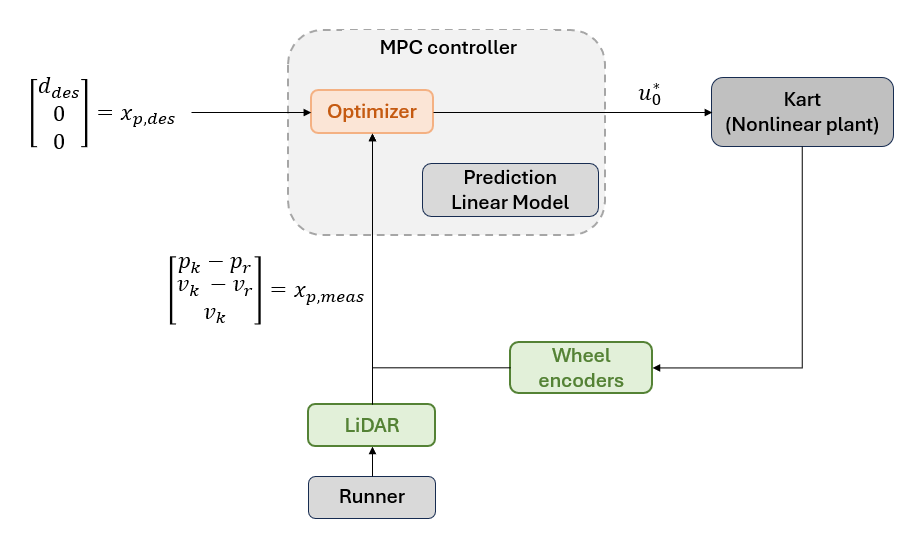
\includegraphics[width=1.0\textwidth]{MPC_hard_scheme.png}
	\caption{Model Predictive Control scheme with sensors}
	\label{image:MPC_hard_scheme}
\end{figure}

In the context of the MPC formulation a similar scheme is employed, with the key difference that the absolute kart velocity $v_k$ information is directly incorporated and utilized in the prediction state, rather than solely by the gain scheduling to switch among controllers, as was the case with the LQR formulation.
The overall scheme is illustrated in figure \ref{image:MPC_hard_scheme} highlighting a simplification of the control architecture compared to the LQR case in figure \ref{image:LQR_hard_scheme}.
In particular, the clip block is removed, and actuator limits are introduced as constraints explicitly in the optimization problem.
Moreover, the two distinct regulators are replaced with a single controller capable of effectively managing the system across various operating conditions.

\bigskip
It is important to notice that the actual absolute runner acceleration, added in the prediction model  \eqref{Prediction_model_MPC} as an affine term, is estimated. 
Initially, the relative acceleration between the kart and runner $\Delta a$ is estimated, alongside the kart's absolute acceleration $a_k$.
The absolute runner acceleration used is then calculated as $a_r = a_k - \Delta a$.

\bigskip
When handling sensor data, such as distance measurements from a LiDAR sensor, it is important to recognize that these measurements are inherently noisy.
In attempting to derive velocity and acceleration from a noisy distance measurement, the situation becomes even more complex since any noise present gets amplified by applying the process of differentiation.
For this reason, even if a Kalman filtering tecnique for smoothing the absolute runner acceleration $a_r$ has been applied, the quality of the estimation result is not accurate enought.
This compromises the MPC's performance compared to simulation results. 
However, despite these challenges, the controller still manages to achieve proper regulation performance concerning the relative distance and position variables.

\begin{algorithm}
\begin{algorithmic}[1]
	\State Define desired prediction state $x_{p,\text{des}} = [d_{\text{des}}, 0, 0]^\top$;
	\State Set initial runner position with a proper distance $\bar{d}$ from kart;
	\For{$t=0,1,2,...$}
		\State Take LiDAR information $\Delta p_t$ and $\Delta v_t$;
		\State Take absolute kart velocity $v_{k,t}$ from wheel encoders;
 		\State Estimate the absolute runner acceleration $a_{r,t}$
		\State $x_{p,t} = [\Delta p_t, \Delta v_t, v_{k,t}]^\top$;
		\State Solve the constrained QP and get $\boldsymbol{u}^* = \{u_0, u_1, \cdots, u_N\}$; 
		\State Inject the first element of the optimal input sequence $u_0^*$ in the plant;
	\EndFor
\caption{MPC implementation on hardware system}
\label{alg:MPC_hard_implementation}
\end{algorithmic}
\end{algorithm}

Algorithm \ref{alg:MPC_hard_implementation} explains the steps followed by the nominal MPC implementation on the hardware system.

\section{Experimental tools}
In this paragraph the tools used for the development of the controllers implementation on the real hardware system are briefly presented.

\subsection*{Robot Operating System}
Robot Operating System (ROS) is an open-source middleware framework specifically designed for robotics research and development  \cite{ros} of robotic applications. 
Despite the name it is not a real operating system but it's a collection of libraries, tools and conventions that allows robotic developers to share, re-use and manage the applications.
Being a communication and middleware layer it serves as an important intermediary layer between the operating system and software applications.
One of the key features of ROS is its modular architecture, which promotes code reuse and modularity by breaking down robot applications into smaller, reusable components called "nodes." 
A node is an individual specific and independent program written in Python or C++ that executes a specific task or function within the framework of a more complex application.
The nodes can communicate with each other using a publish-subscribe messaging system, allowing for flexible and decentralized control architectures. 
In particular nodes can publish messages to topics (publisher) and other nodes can subscribe to these topics to receive and process the data (suscriber).


\bigskip
ROS, and in particular its successor ROS 2, offers numerous features and improvements that make it well-suited for driving autonomous systems and automated driving projects.
At the core of ROS 2's functionality lies the ability to run directly on the onboard computer of autonomous systems, having Ubuntu pre-installed, processing raw data coming from sensors and executing the proper control algorithms.
In this sense, one of the most notable innovations in ROS 2 is its ability to support real-time capabilities, of fundamental importance when autonomous systems have to perform safety-critical and time-sensitive applications.


\subsection*{Docker}
Docker is an open-source platform that enables developers to package, distribute, and run applications in lightweight, portable containers. 
These containers encapsulate all the dependencies and runtime components needed to run an application, including the code, system tools, libraries, and settings.
Docker containers are designed to be isolated from each other and from the underlying host system, ensuring consistent and reliable execution across different environments.
The only thing preventing a container from being able to stand alone is that it relies on the host’s operating system (OS) and kernel for low-level services, such as resource management and network access.
\begin{figure}
	\centering
	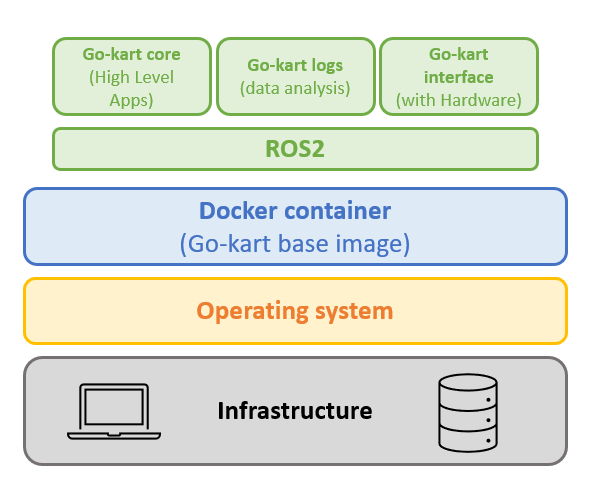
\includegraphics[width=0.5\textwidth]{Docker.png}
	\caption{Docker}
	\label{image:Docker}
\end{figure}

\subsection*{Go-kart repository}
The autonomous go-kart repository consists of four different images. 
The first one is the Ubuntu 20.04 base image with ROS 2 installed and is the base for the other go-kart repositories stack.
This layer manages the installation of the common libraries and the ROS 2 communication between the hardware components (sensors and actuators) and the software applications contained in the other three higher-level images. 
The communication is achieved through the ad-hoc definition of messages.

The go-kart logs is the repository responsible for data analysis. 
Specifically, it interprets and decodes binary sensor data into a numerical format that is meaningful and can be understood and processed by other software applications, such as control algorithms.
In this application, binary signals are converted into CSV files.

The go-kart interface repository is responsible for interfacing with hardware, serving as the intermediary layer between the operating system and the hardware. 
Drivers read messages from ROS topics, enabling hardware components (such as LiDAR, cameras, motors, etc.) to execute requested actions.

Finally, the go-kart core contains all the high level applications, such as the controller. 
Several C++ packages for estimation, control, or visualization exist in order to execute various tasks in a modular and reusable manner.

\subsection*{CasADi and qrSQP solver}
For the hardware implementation of the ROS 2 controllers packages, CasADI together with qrSQP solver were utilized.
CasADi (Computer Algebra System for Automatic Differentiation) \cite{Andersson2018} serves as a symbolic framework designed for automatic differentiation and numerical optimization.
It facilitates the representation of mathematical expressions symbolically, crucial for modeling complex control systems efficiently.


\section{Hardware-in-the-loop implementation and tests}
In this section some hardware-in-the-loop tests developed are presented and analyzed.
First of all the model utilized for the controllers development has been demostrated to reproduce enough accurately the behaviour of the system when moving rectilinearly.

\begin{figure} 
    \centering
    \begin{subfigure}[b]{0.32\textwidth}
        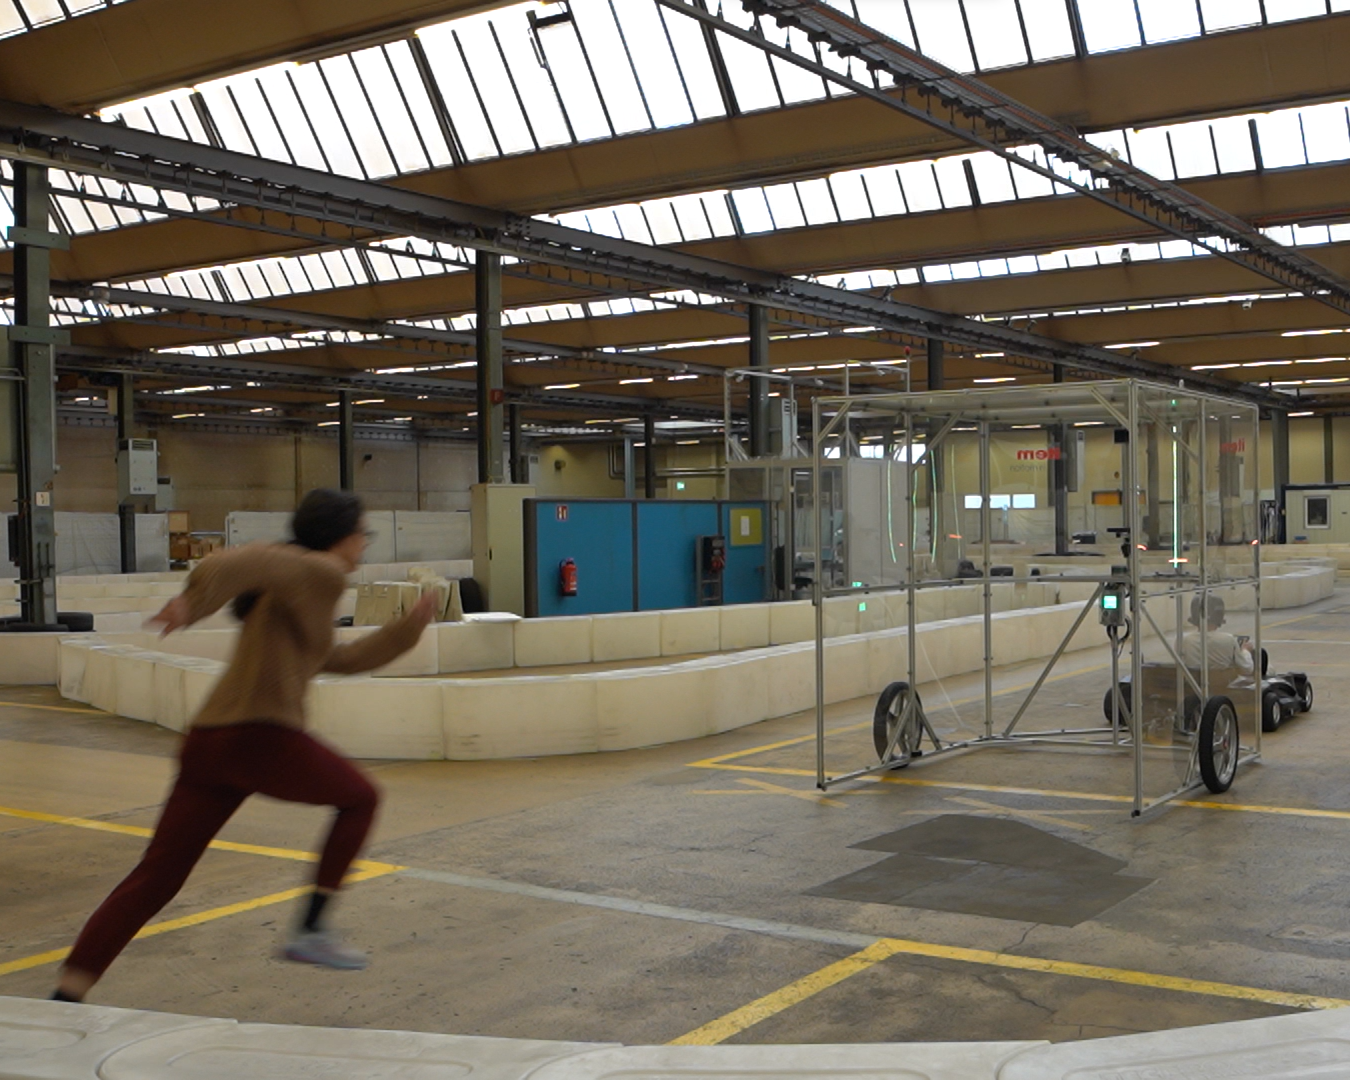
\includegraphics[width=\textwidth]{Catch/Catch1.png}
    \end{subfigure}
    \hfill
    \begin{subfigure}[b]{0.32\textwidth}
        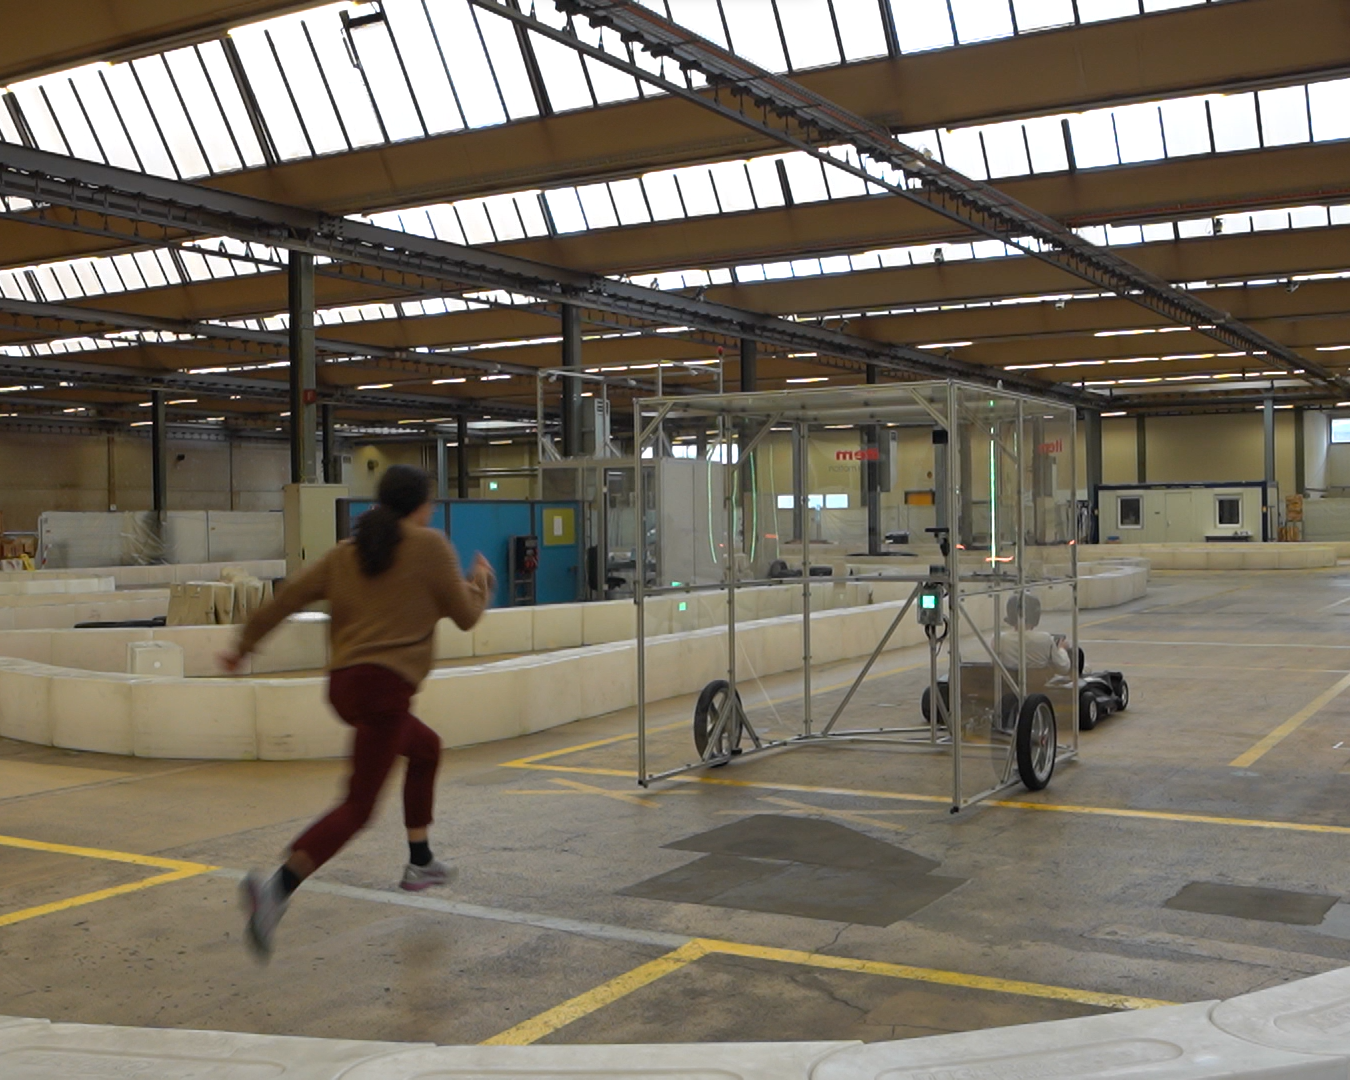
\includegraphics[width=\textwidth]{Catch/Catch2.png}
    \end{subfigure}
    \hfill
    \begin{subfigure}[b]{0.32\textwidth}
        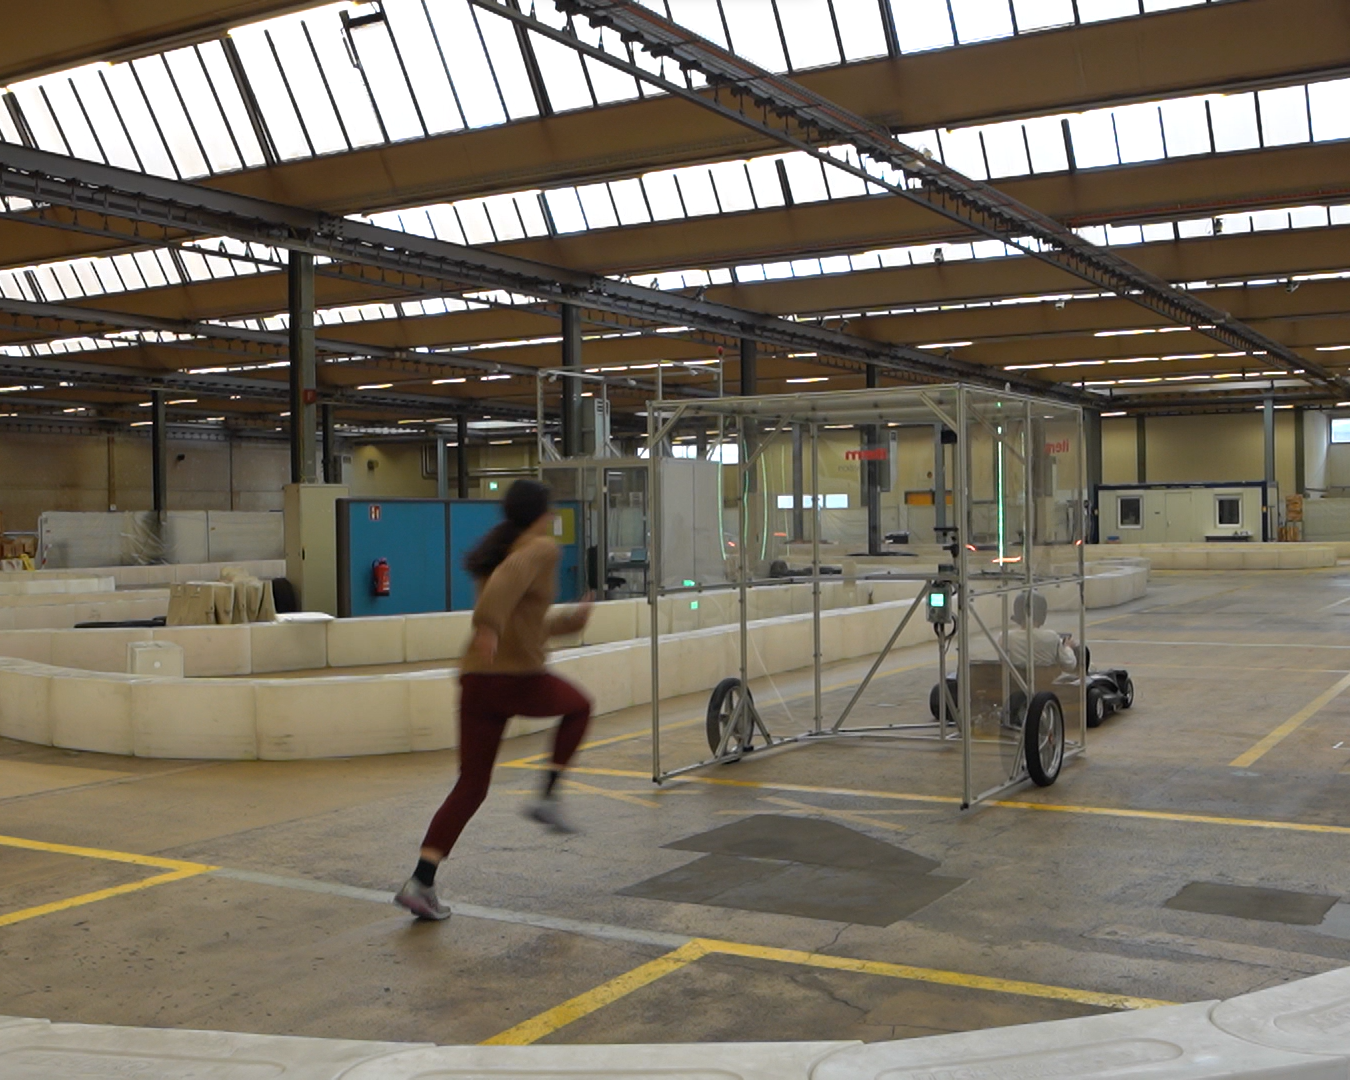
\includegraphics[width=\textwidth]{Catch/Catch3.png}
    \end{subfigure}
    \\[0.2cm]
    \begin{subfigure}[b]{0.32\textwidth}
        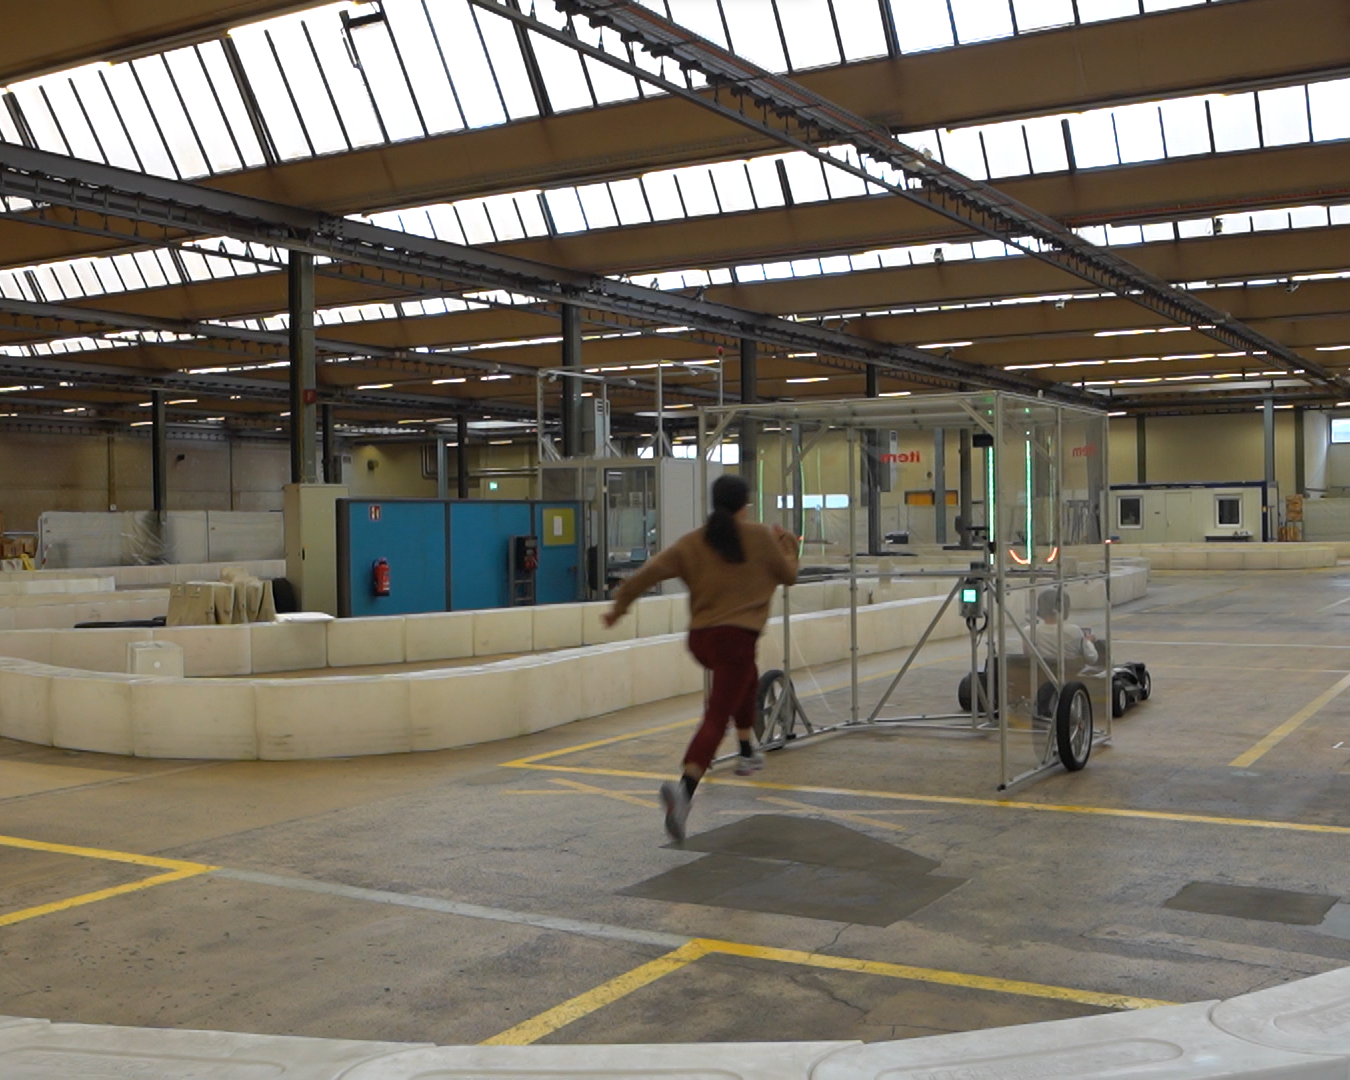
\includegraphics[width=\textwidth]{Catch/Catch4.png}
    \end{subfigure}
    \hfill
    \begin{subfigure}[b]{0.32\textwidth}
        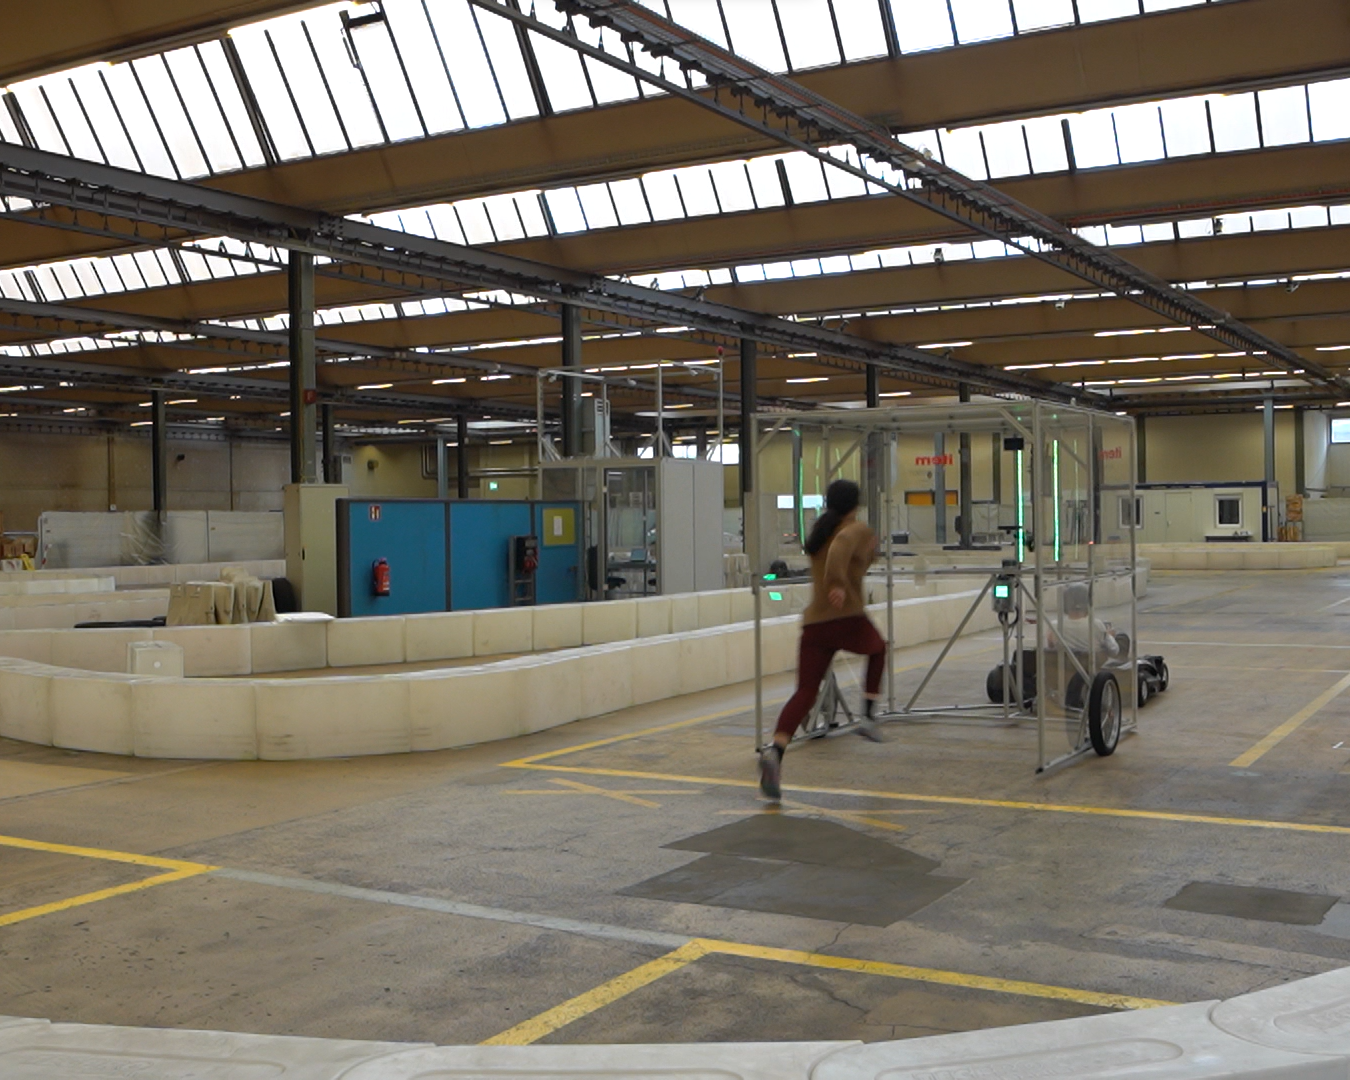
\includegraphics[width=\textwidth]{Catch/Catch5.png}
    \end{subfigure}
    \hfill
    \begin{subfigure}[b]{0.32\textwidth}
        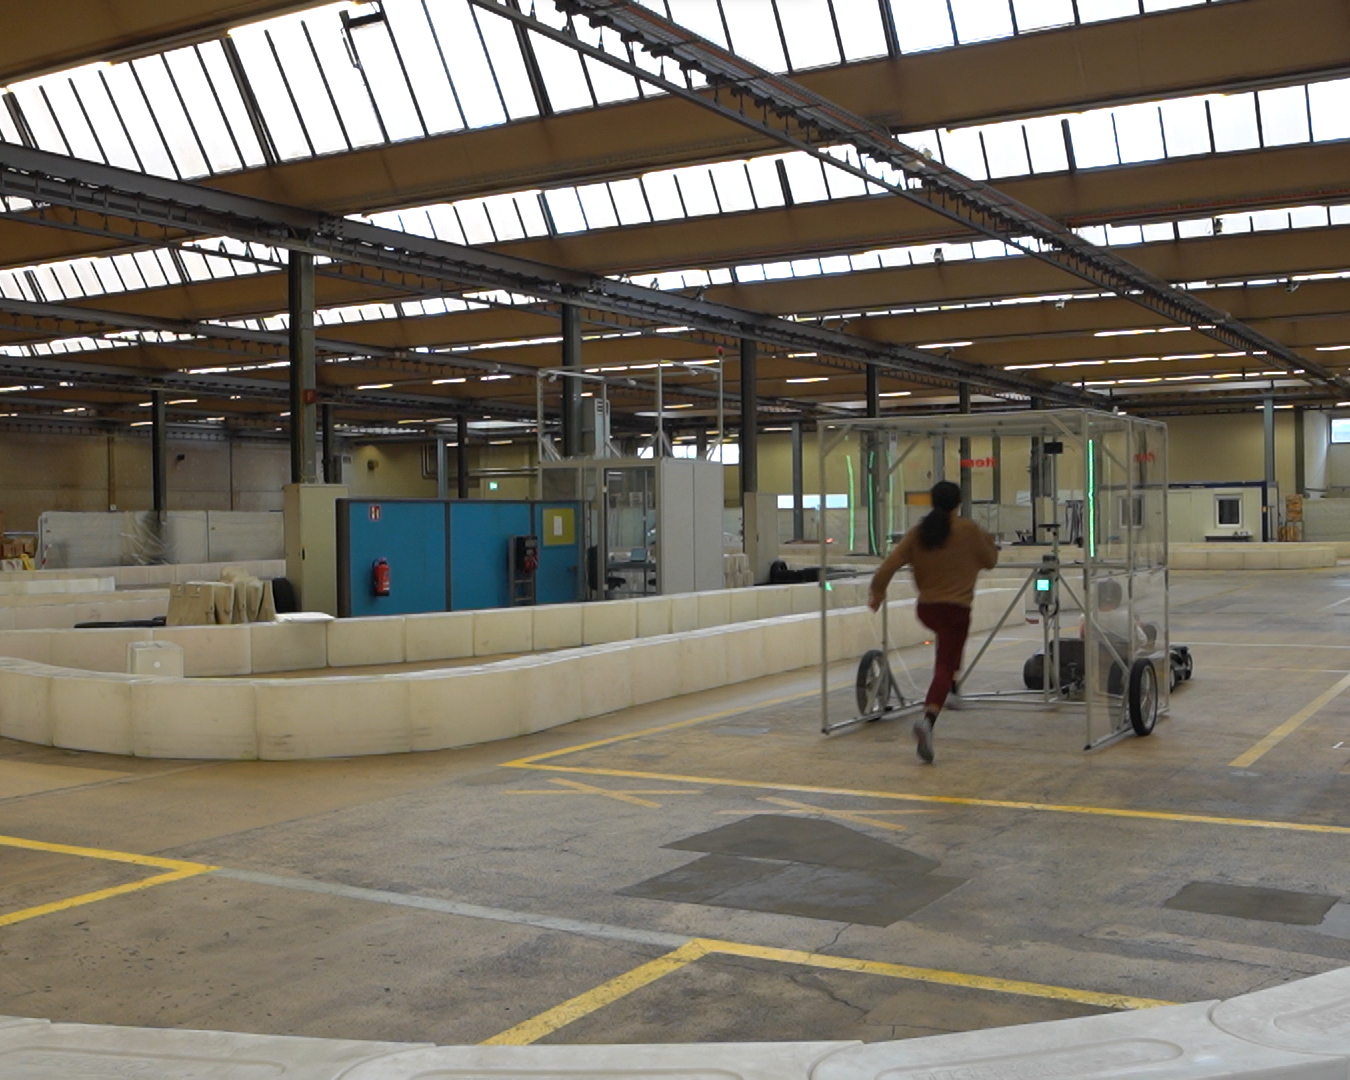
\includegraphics[width=\textwidth]{Catch/Catch6.png}
    \end{subfigure}
    \\[0.2cm]
    \begin{subfigure}[b]{0.32\textwidth}
        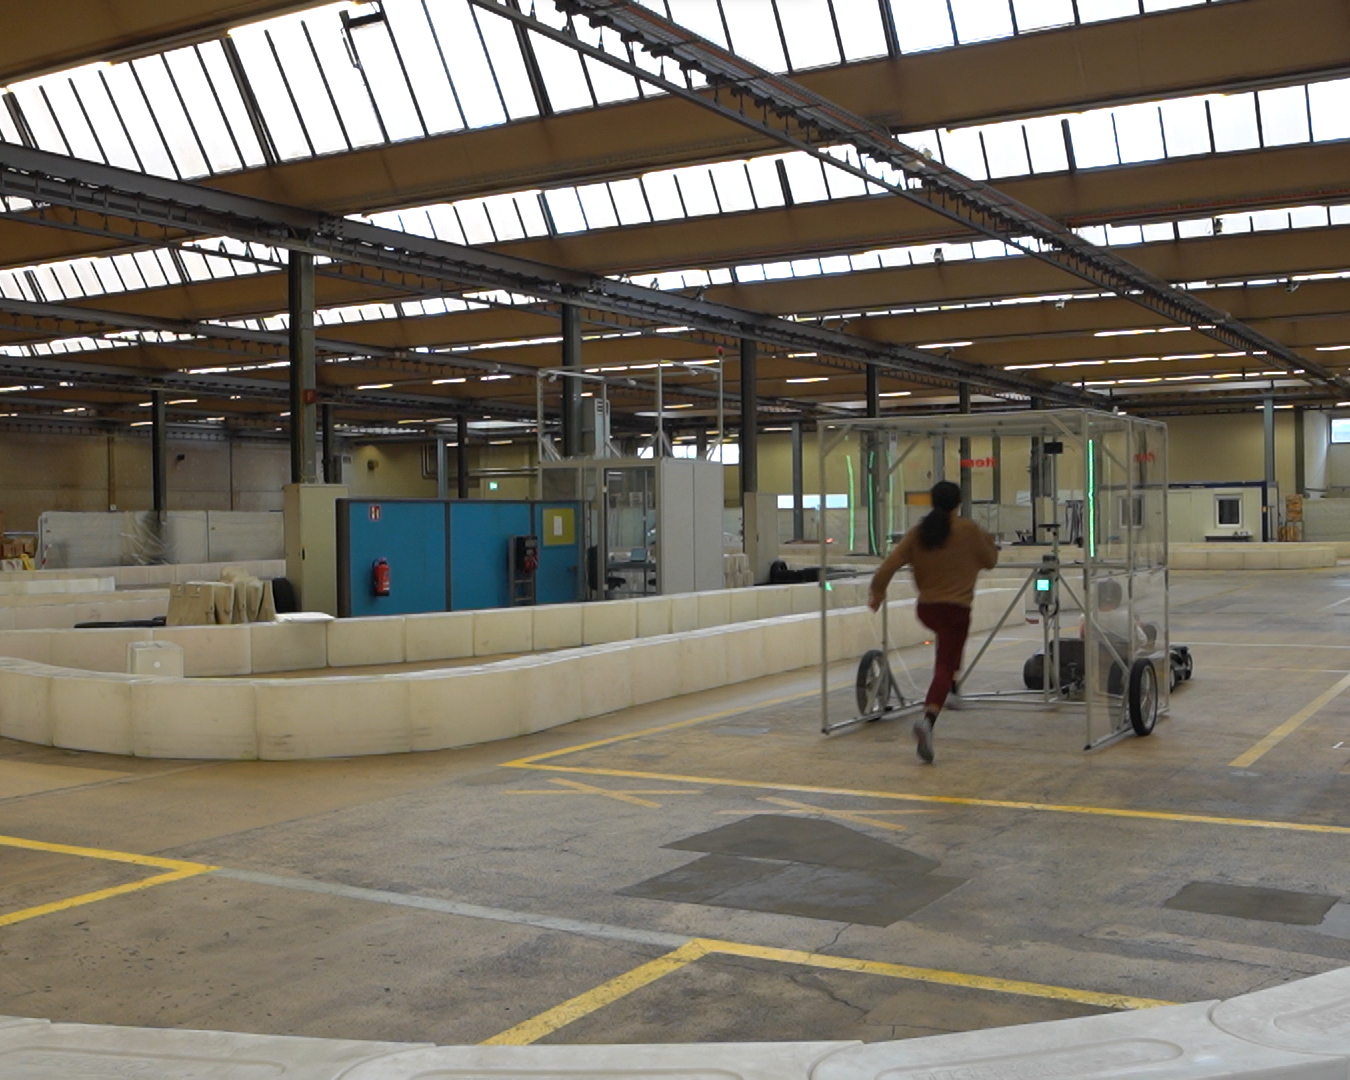
\includegraphics[width=\textwidth]{Catch/Catch7.png}
    \end{subfigure}
    \hfill
    \begin{subfigure}[b]{0.32\textwidth}
        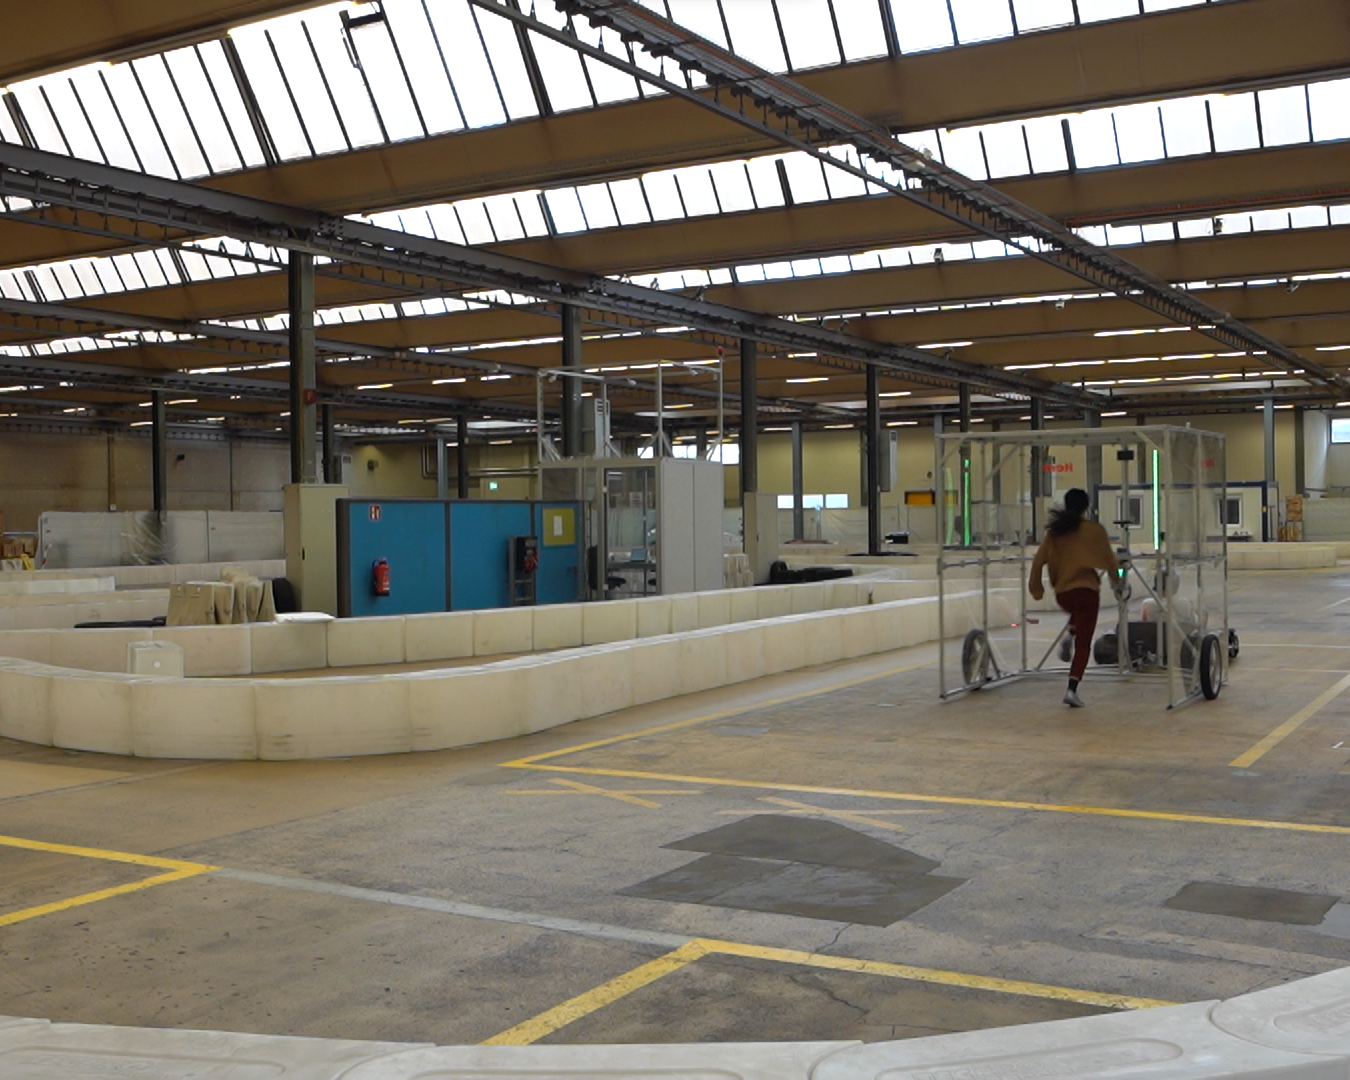
\includegraphics[width=\textwidth]{Catch/Catch8.png}
    \end{subfigure}
    \hfill
    \begin{subfigure}[b]{0.32\textwidth}
        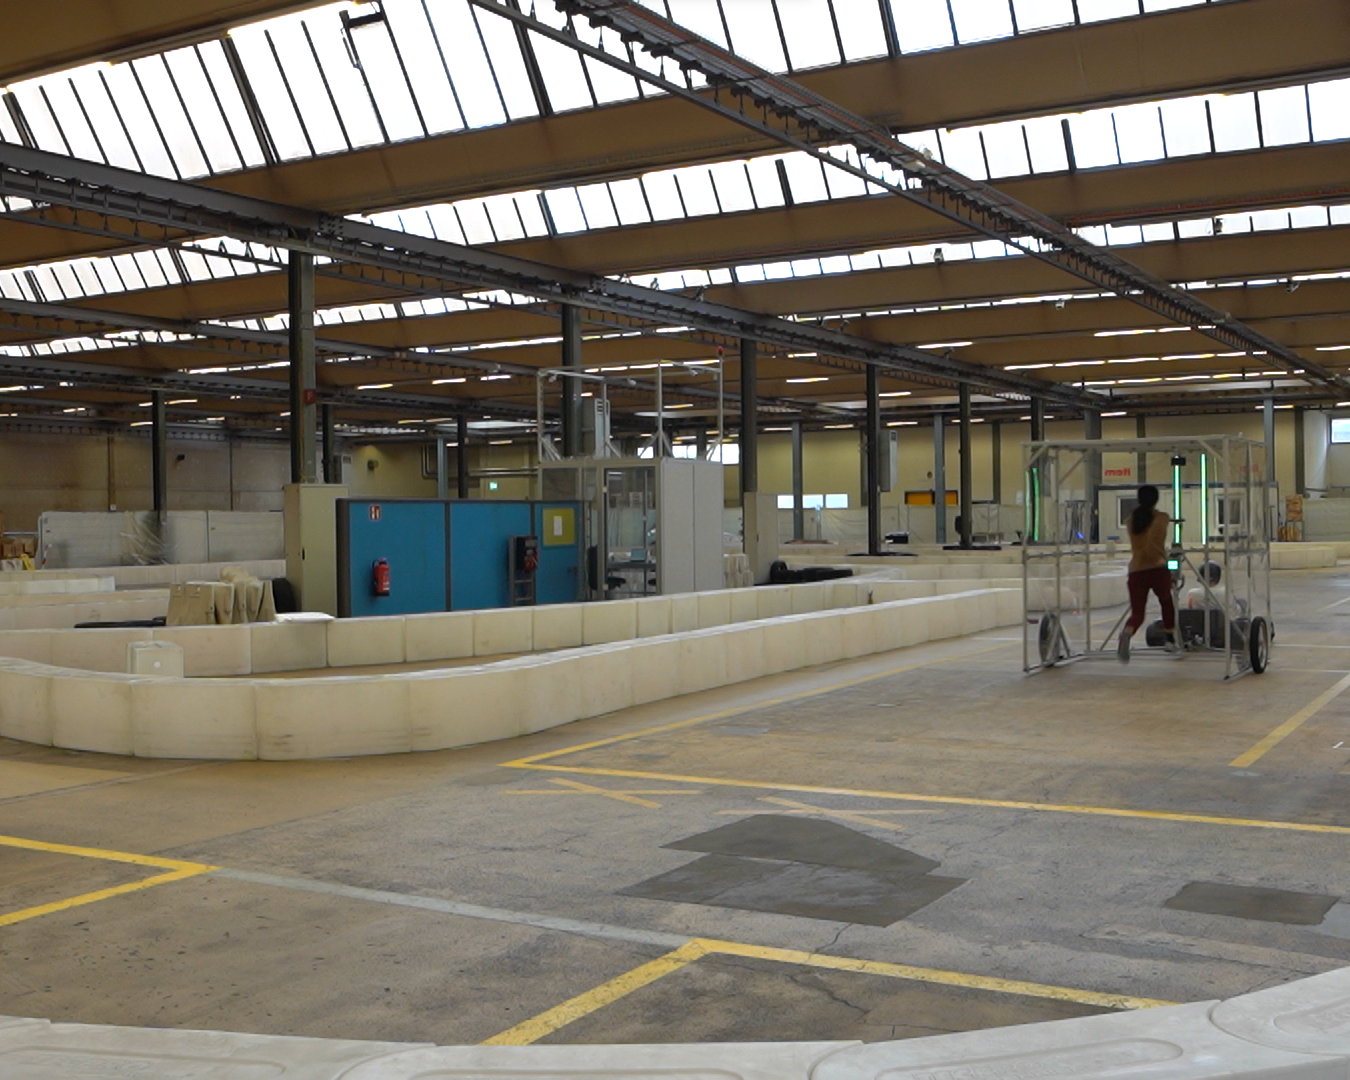
\includegraphics[width=\textwidth]{Catch/Catch9.png}
    \end{subfigure}
    \caption{Sequence of images taken from a video, showing a catch-up maneuver regulated with MPC }
\label{MPC_hard_img1}
\end{figure}

\bigskip
The sequence of images in figure \ref{MPC_hard_img1} are taken from a video, recording the behaviour of the nominal Model Predictive Controller running on the real system.
It can be noticed, from the first line of images, that the runner has started the sprint some meters further from the border of the airshield.
Accorgingly, the focus of the test was on the first phase of the motion that is accomplished in a safe manner.


\begin{figure}
    \centering
    \begin{subfigure}[b]{0.32\textwidth}
        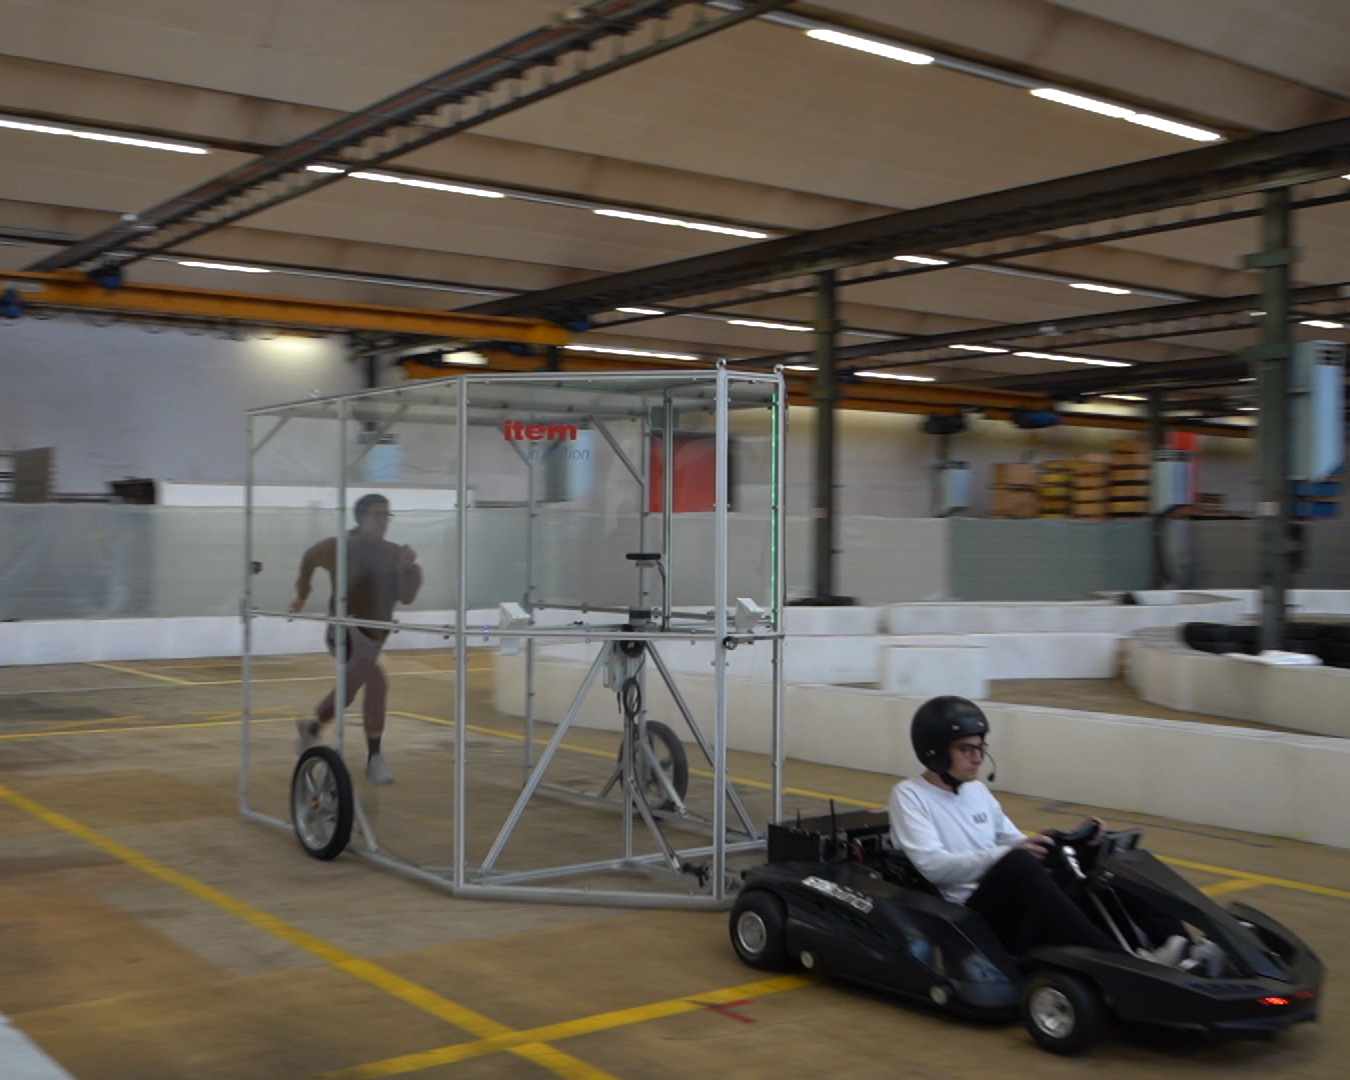
\includegraphics[width=\textwidth]{SteadyState/ss1.png}
    \end{subfigure}
    \hfill
    \begin{subfigure}[b]{0.32\textwidth}
        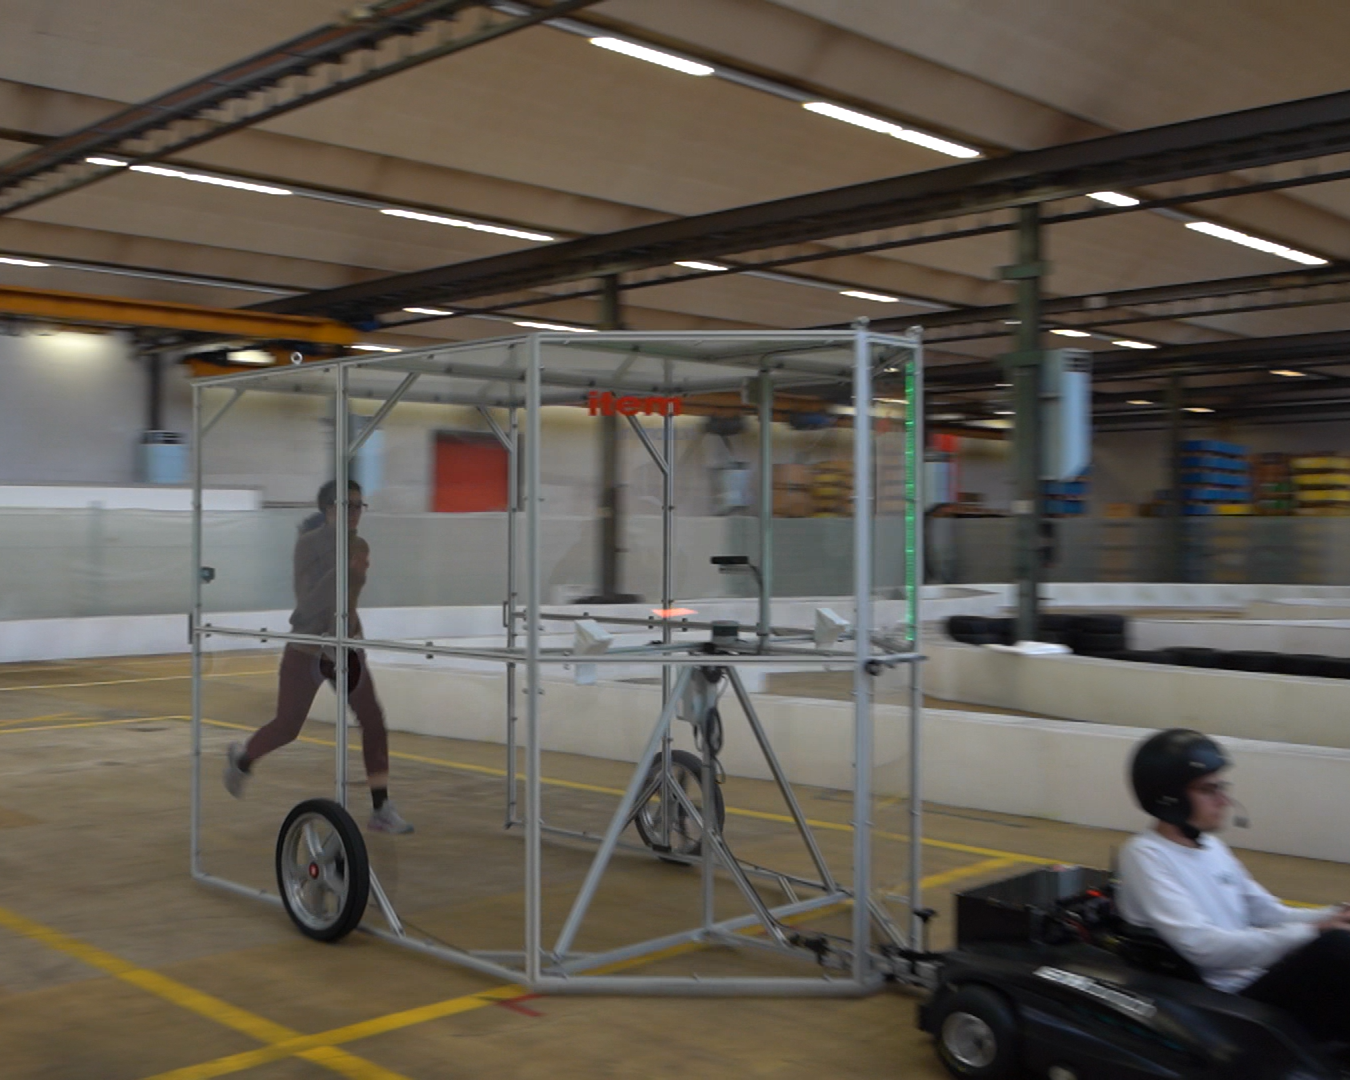
\includegraphics[width=\textwidth]{SteadyState/ss2.png}
    \end{subfigure}
    \hfill
    \begin{subfigure}[b]{0.32\textwidth}
        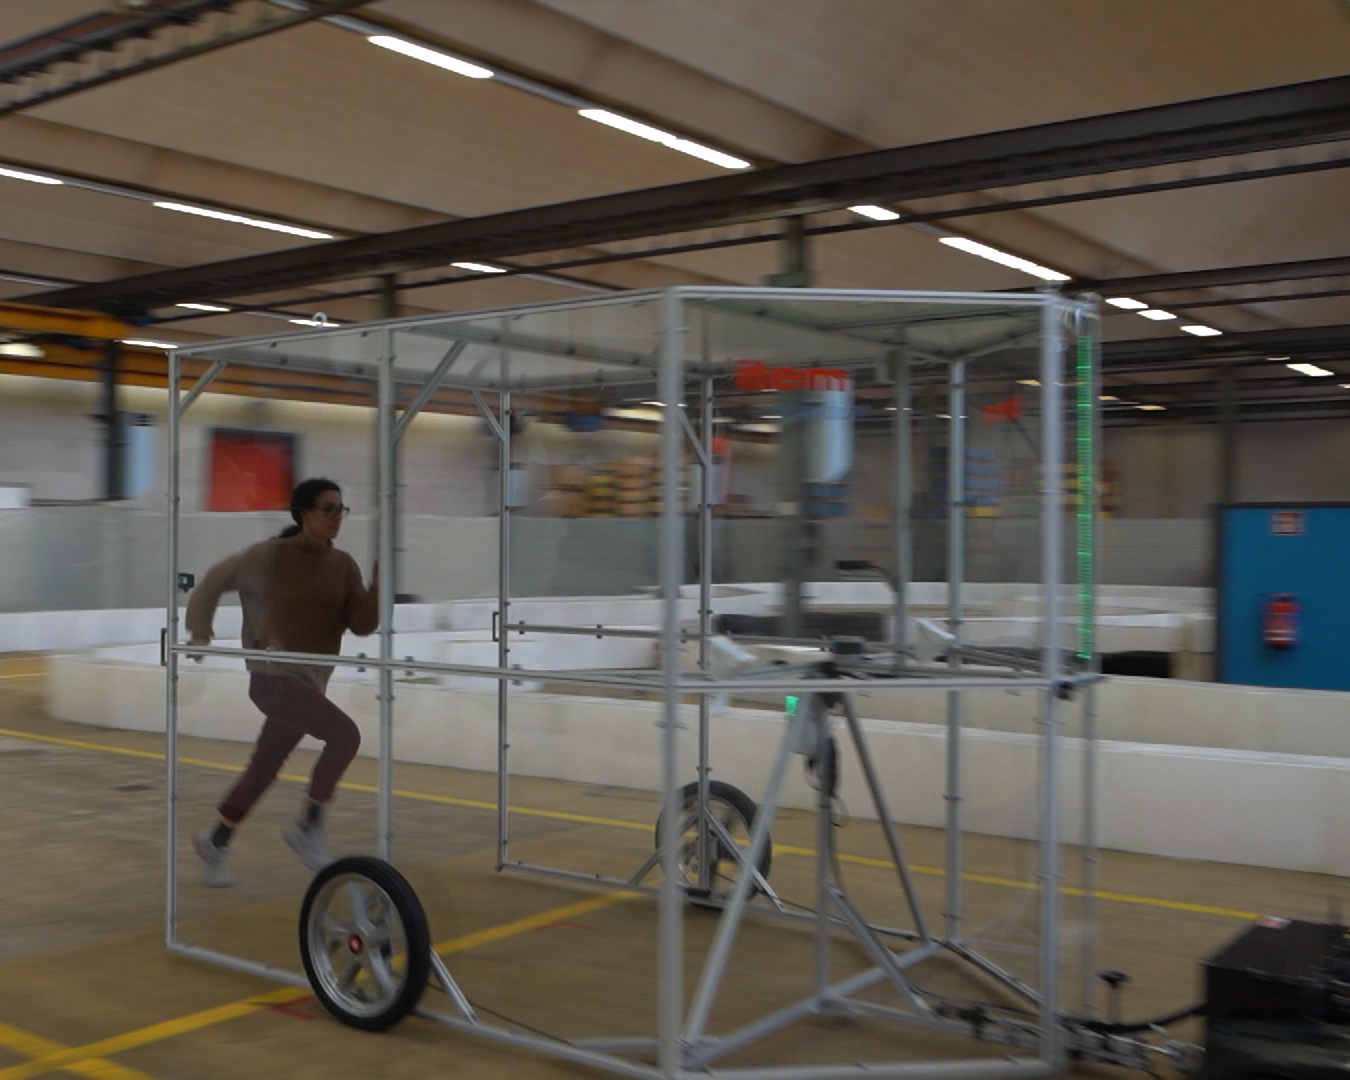
\includegraphics[width=\textwidth]{SteadyState/ss3.png}
    \end{subfigure}
    \\[0.2cm]
    \begin{subfigure}[b]{0.32\textwidth}
        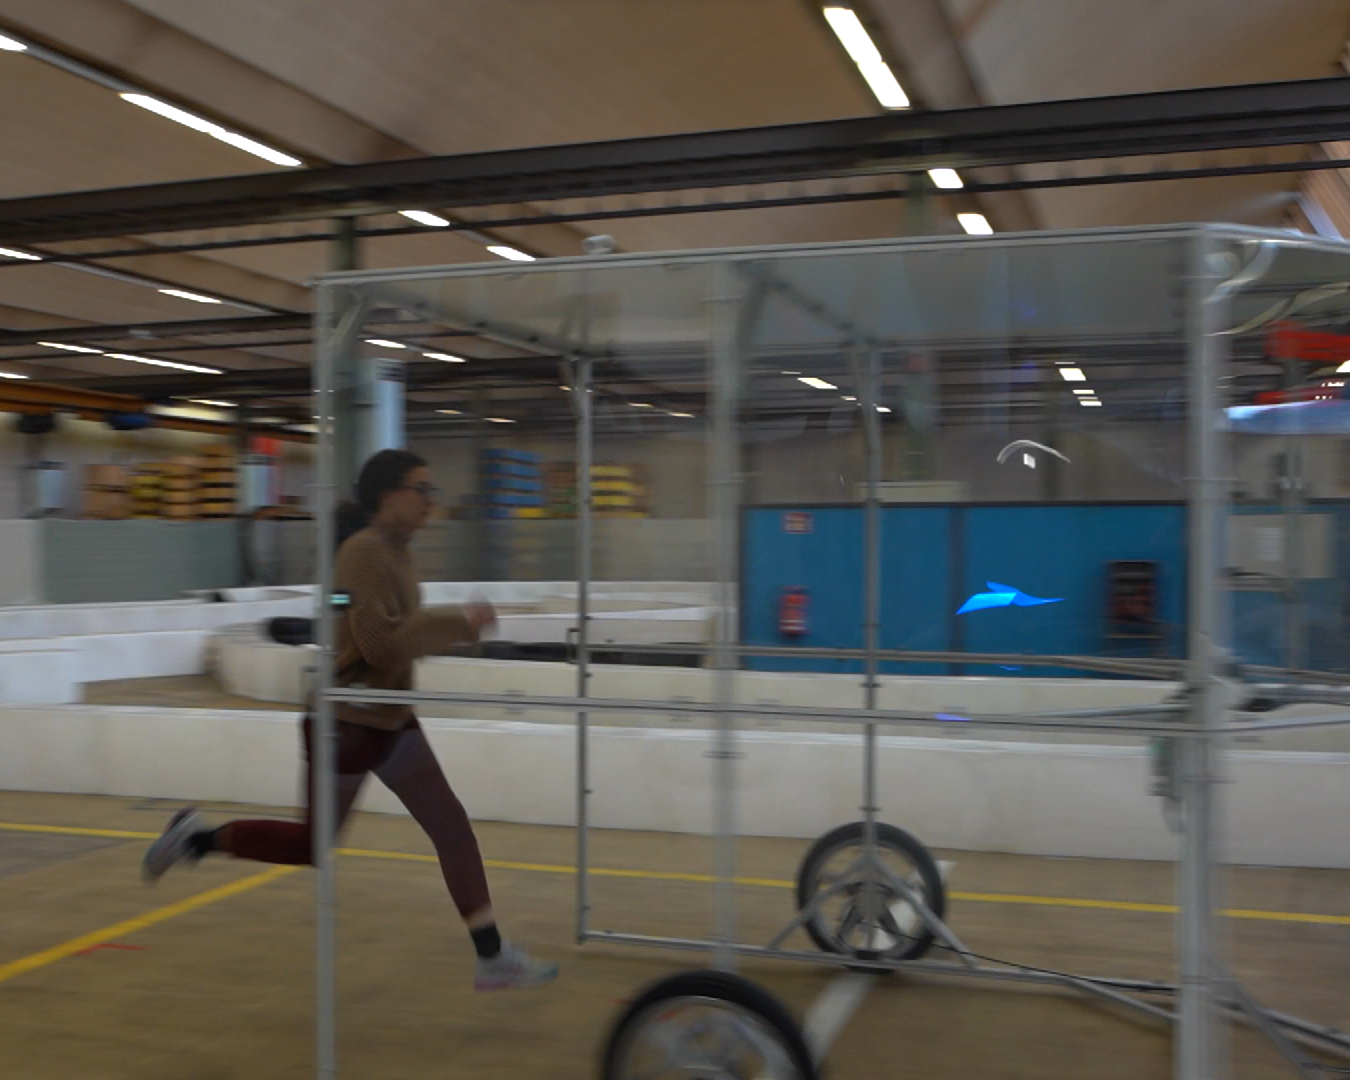
\includegraphics[width=\textwidth]{SteadyState/ss4.png}
    \end{subfigure}
    \hfill
    \begin{subfigure}[b]{0.32\textwidth}
        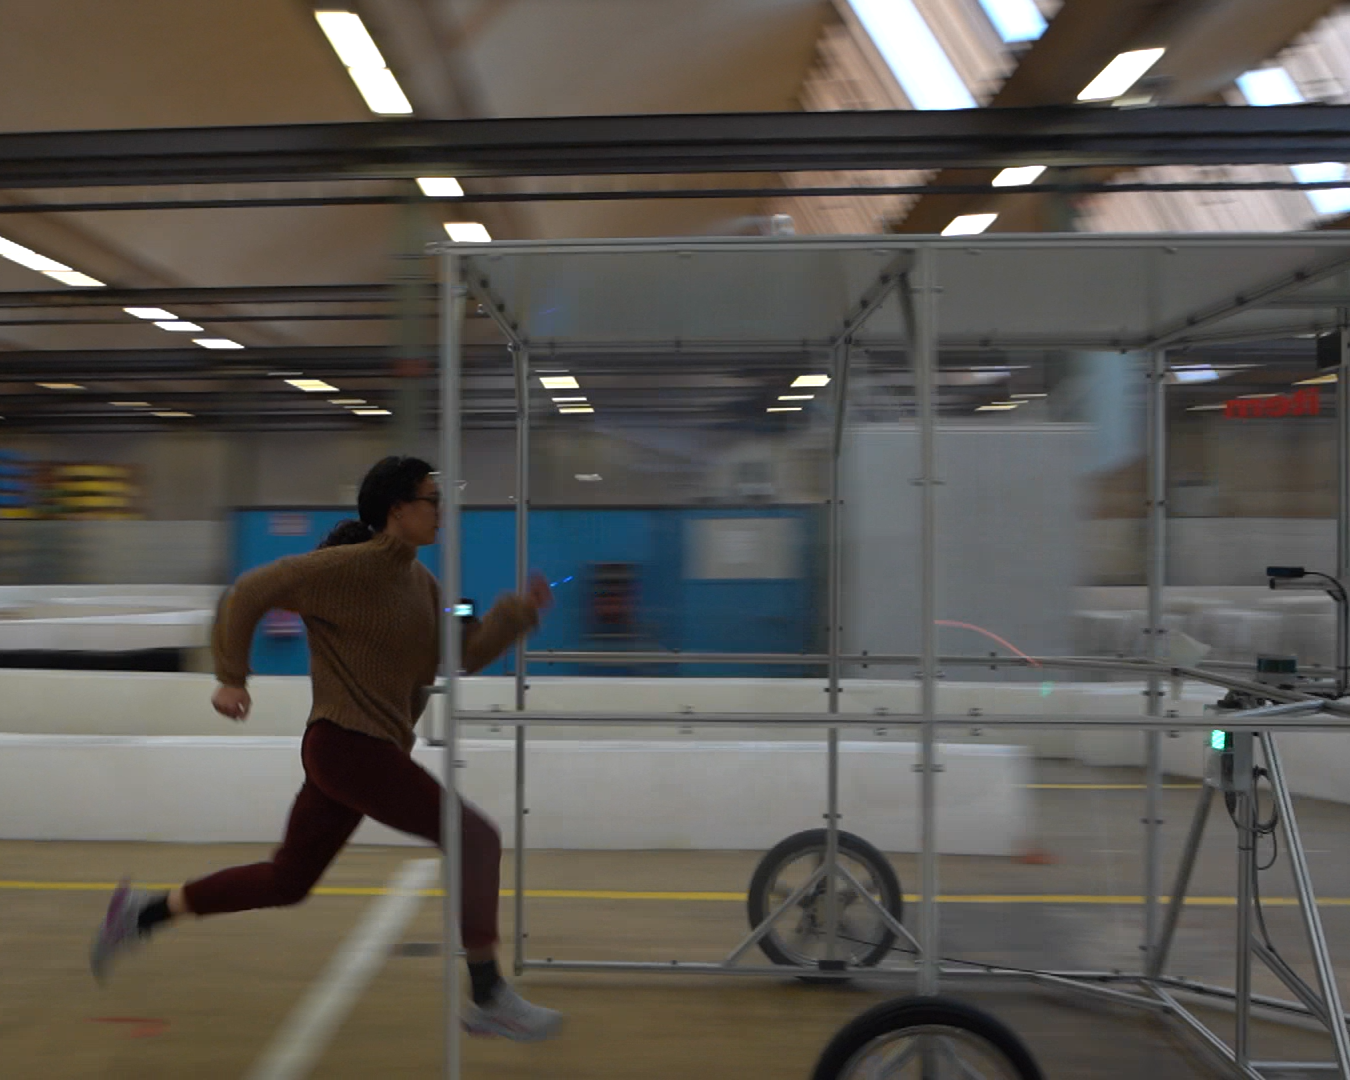
\includegraphics[width=\textwidth]{SteadyState/ss5.png}
    \end{subfigure}
    \hfill
    \begin{subfigure}[b]{0.32\textwidth}
        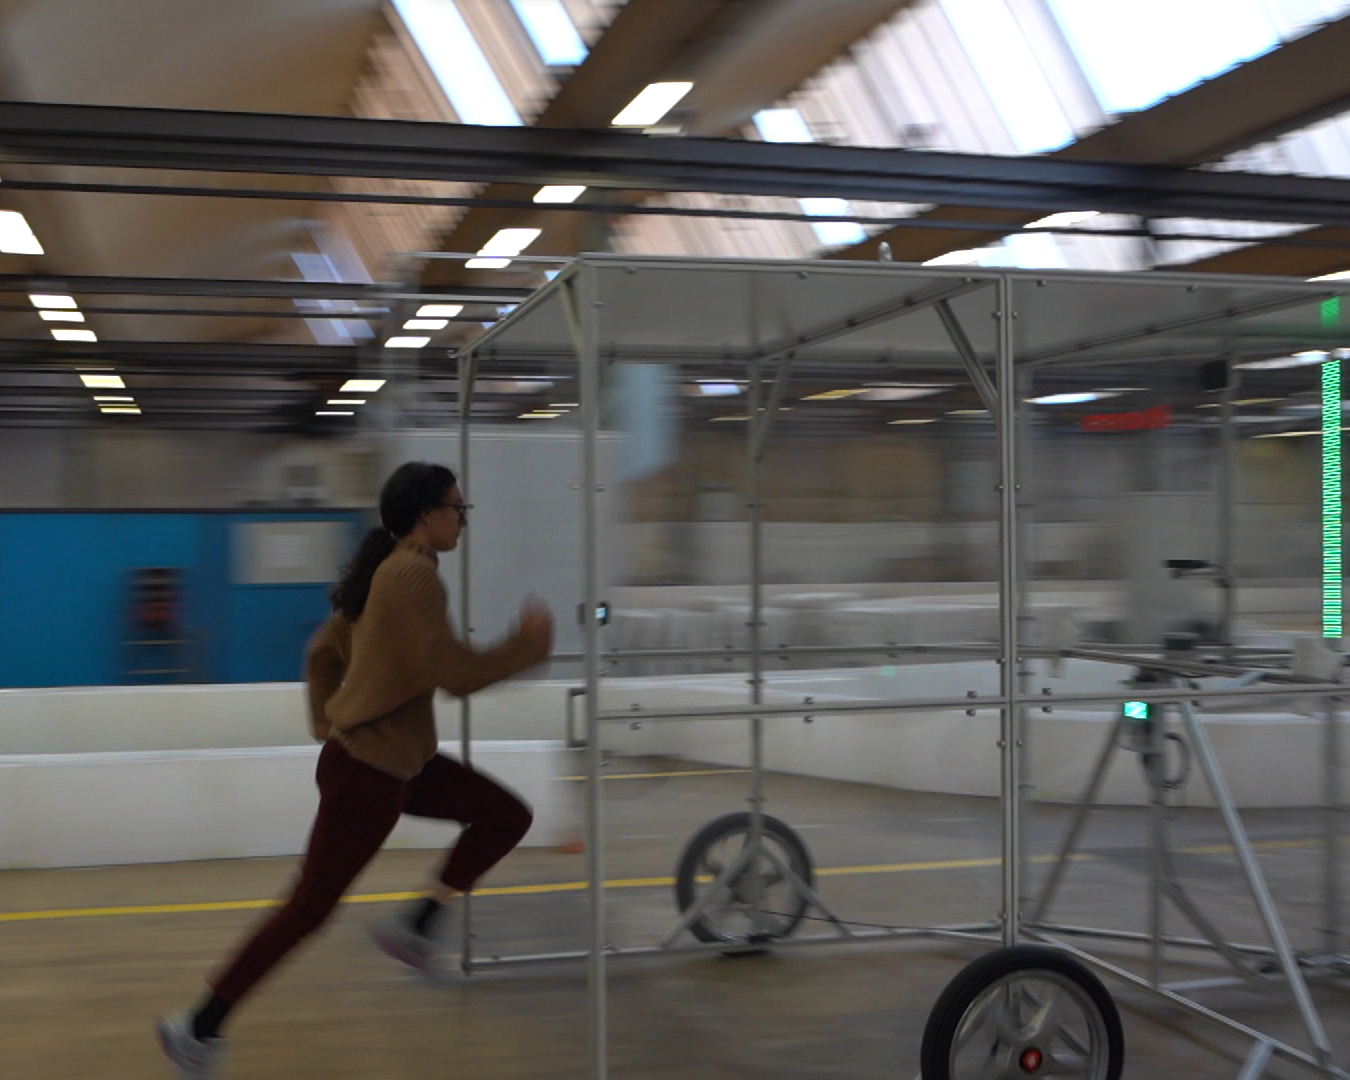
\includegraphics[width=\textwidth]{SteadyState/ss6.png}
    \end{subfigure}
    \\[0.2cm]
    \begin{subfigure}[b]{0.32\textwidth}
        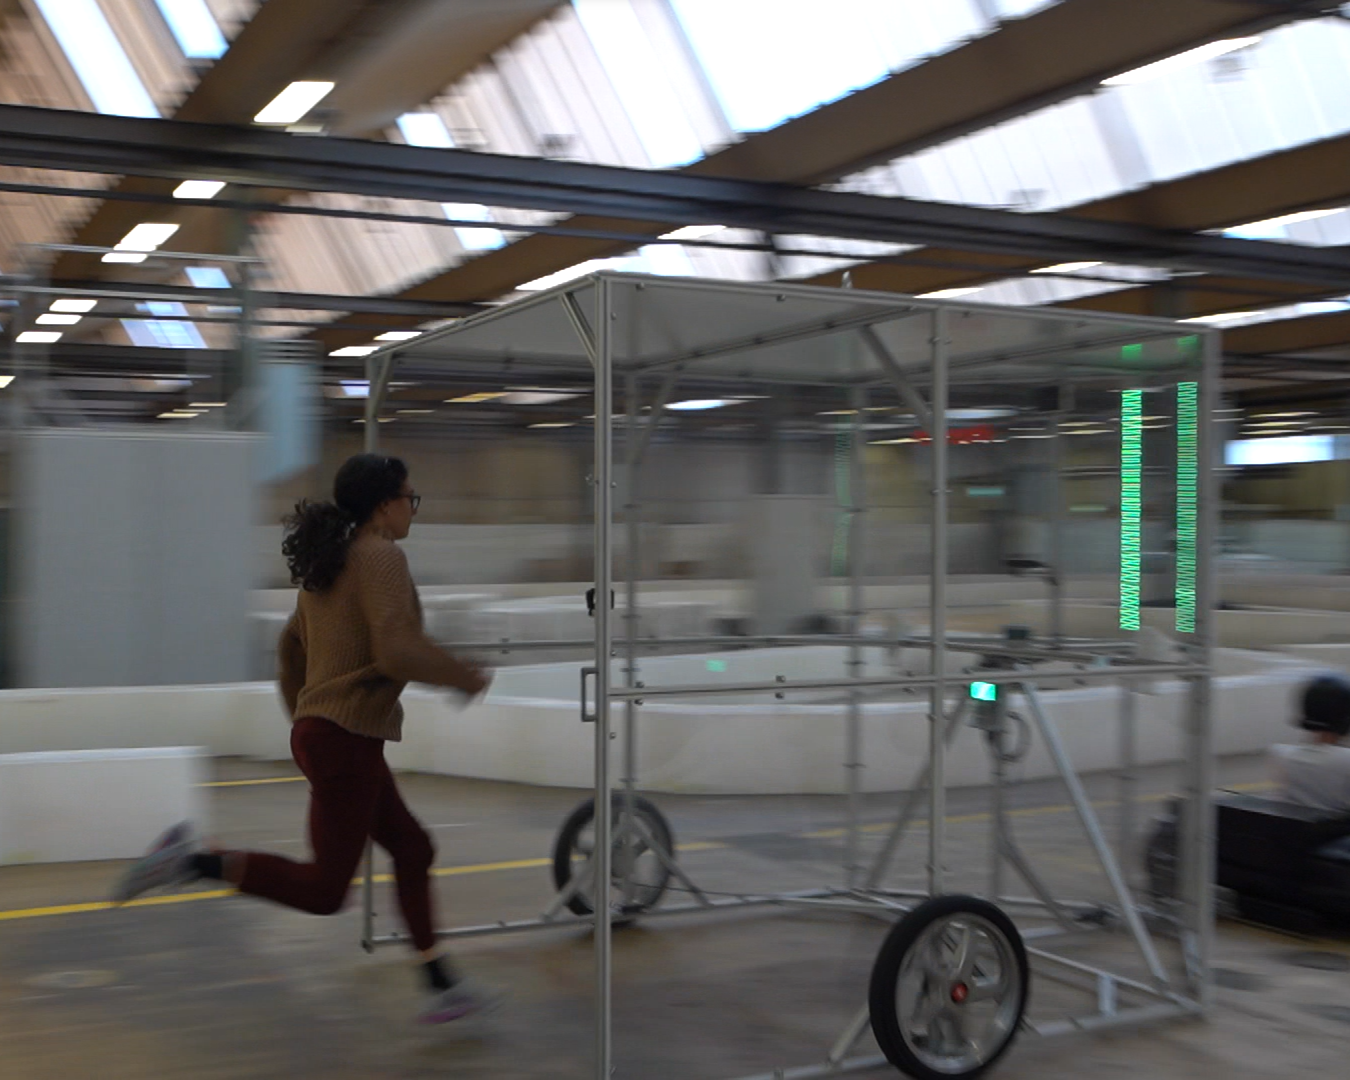
\includegraphics[width=\textwidth]{SteadyState/ss7.png}
    \end{subfigure}
    \hfill
    \begin{subfigure}[b]{0.32\textwidth}
        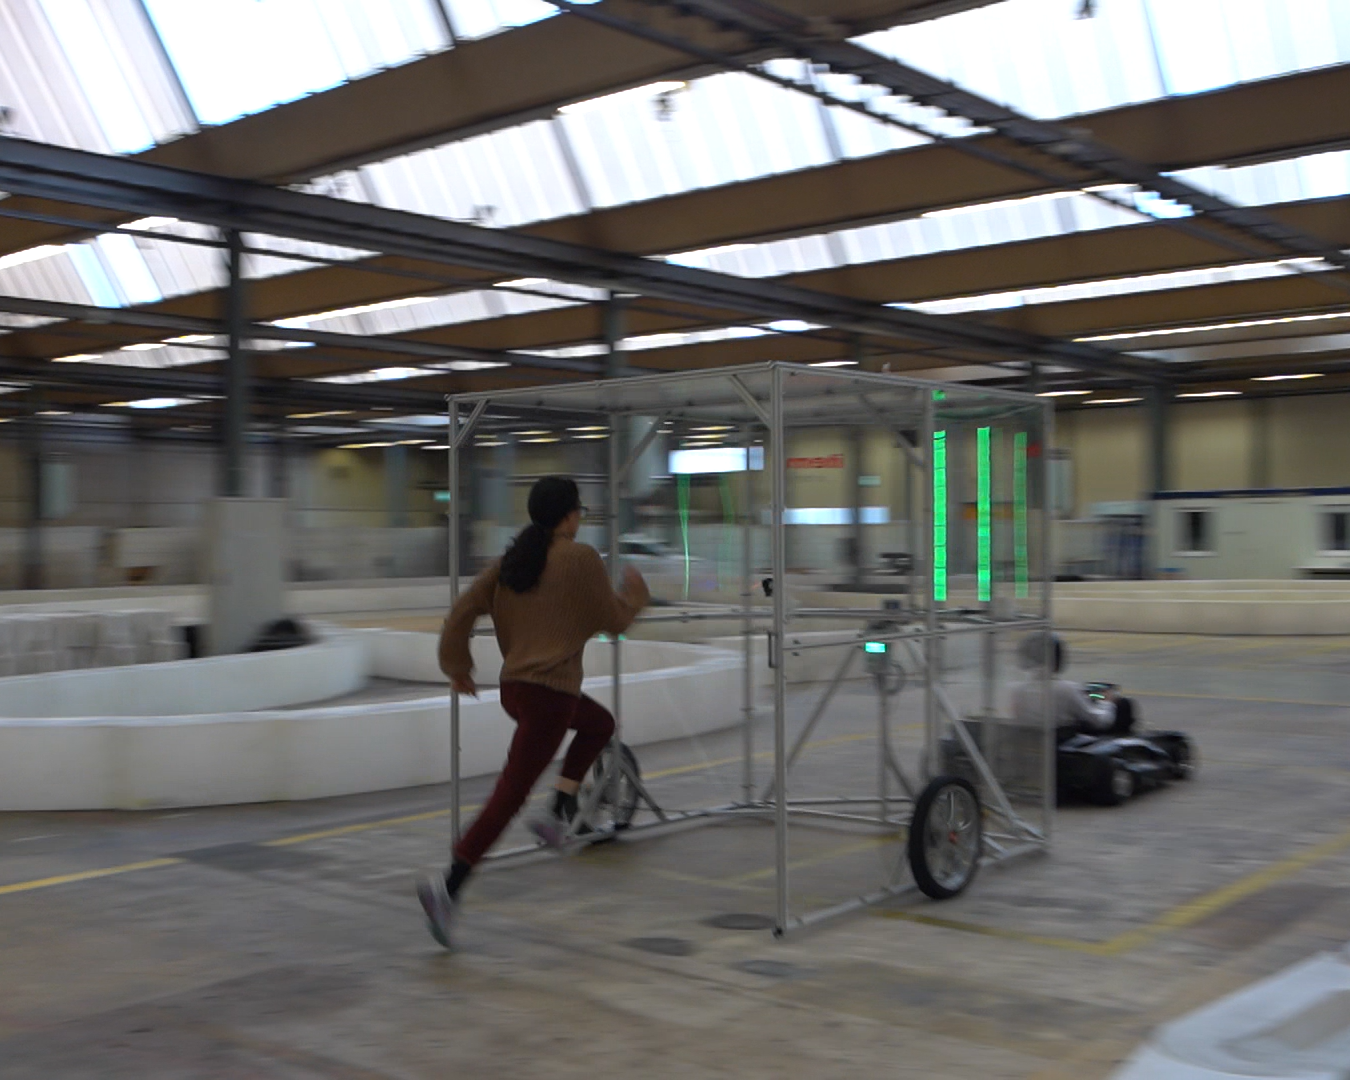
\includegraphics[width=\textwidth]{SteadyState/ss8.png}
    \end{subfigure}
    \hfill
    \begin{subfigure}[b]{0.32\textwidth}
        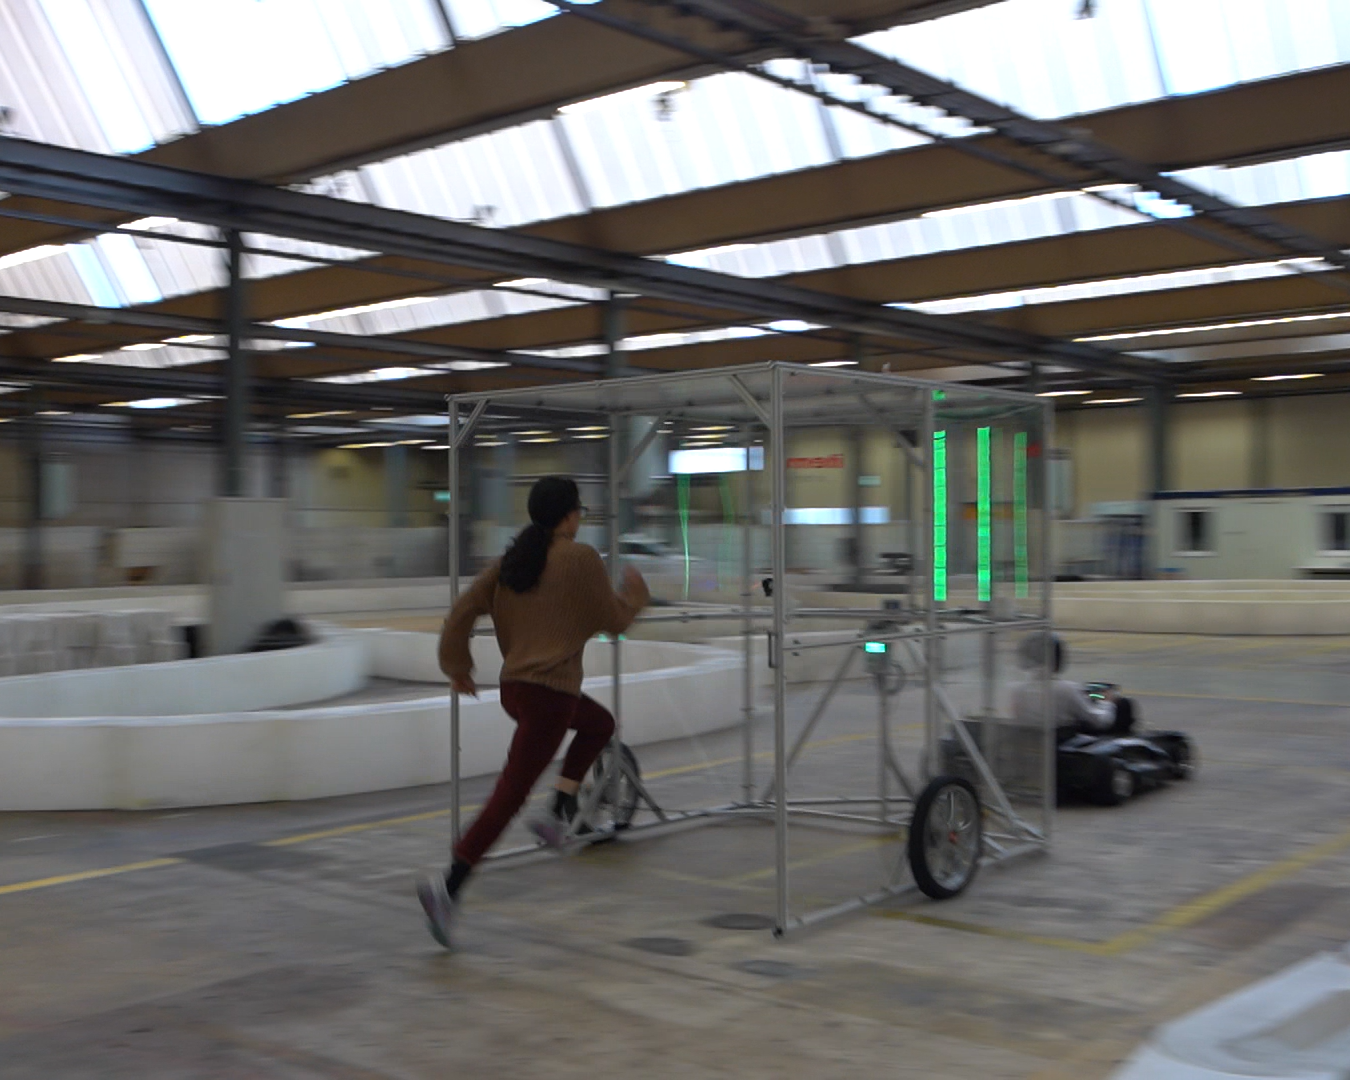
\includegraphics[width=\textwidth]{SteadyState/ss9.png}
    \end{subfigure}
    \caption{Sequence of images taken from a video, showing a tracking regulated with MPC }
\label{MPC_hard_img2}
\end{figure}


\begin{figure}
    \centering
    \begin{subfigure}[t]{0.7\textwidth}
        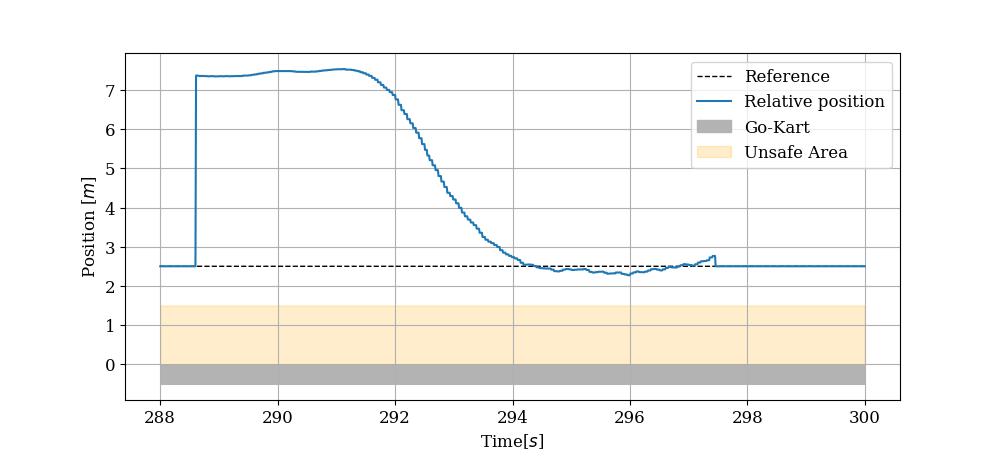
\includegraphics[width=\textwidth]{Hardware_testMPC/Position.png}
        \caption{Relative position between runner and go-kart}
        \label{fig:Deltaphard}
    \end{subfigure}
    
    \begin{subfigure}[t]{0.7\textwidth}
        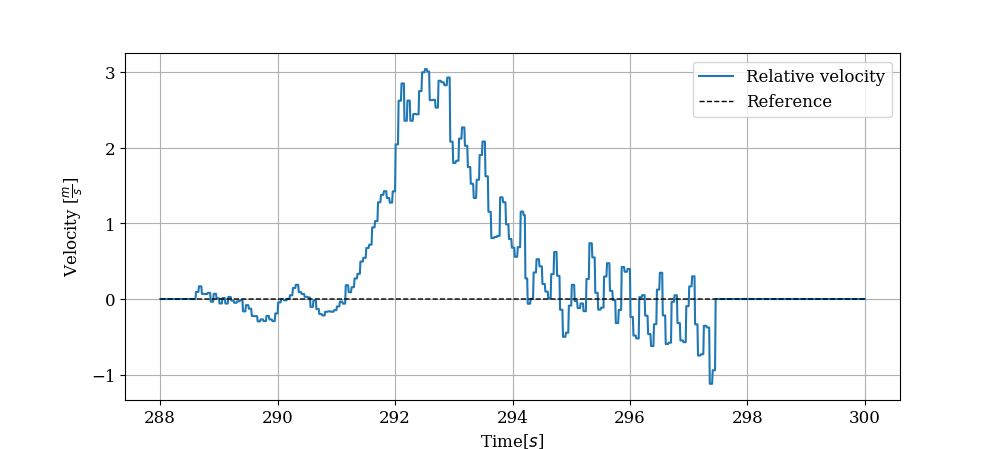
\includegraphics[width=\textwidth]{Hardware_testMPC/Velocity.png}
        \caption{Relative velocity between runner and go-kart}
        \label{fig:Deltavhard}
    \end{subfigure}
    
    \begin{subfigure}[t]{0.7\textwidth}
        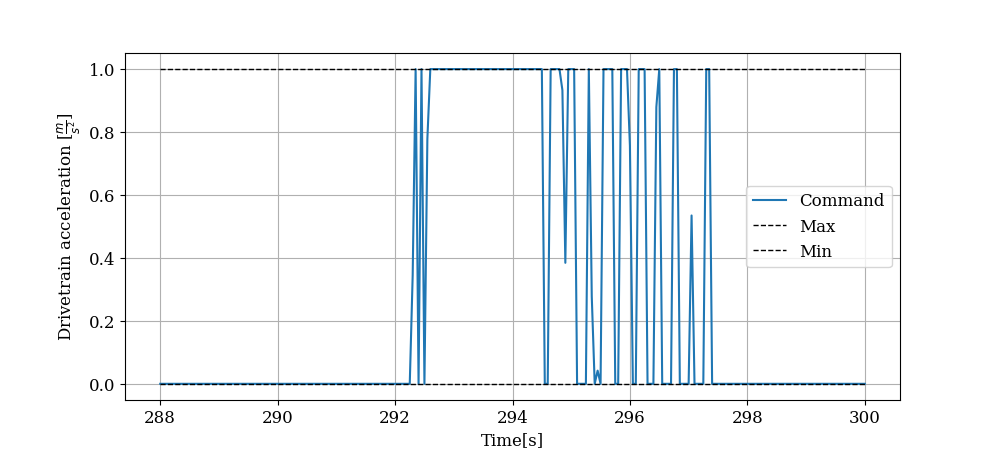
\includegraphics[width=\textwidth]{Hardware_testMPC/Input.png}
        \caption{Input effort (drive-train acceleration)}
        \label{fig:Inputhard}
    \end{subfigure}

    \begin{subfigure}[t]{0.7\textwidth}
        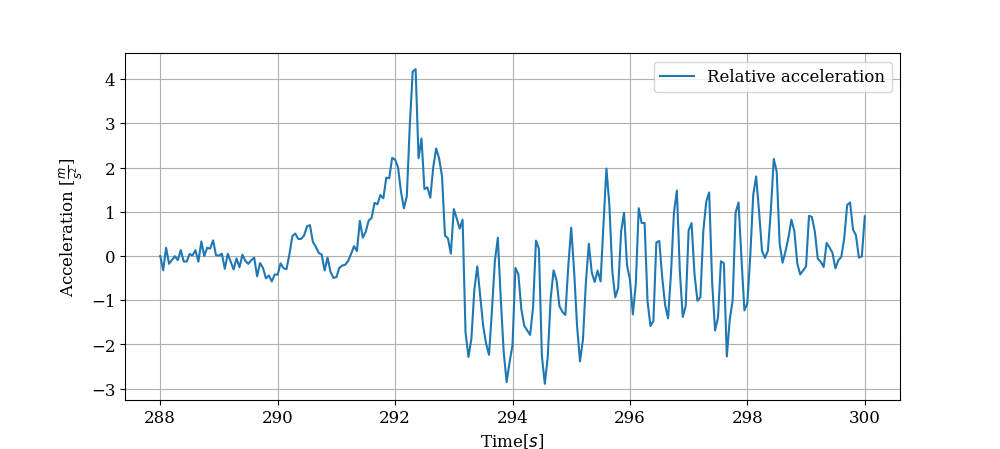
\includegraphics[width=\textwidth]{Hardware_testMPC/Acceleration.png}
        \caption{Estimated Acceleration}
        \label{fig:Est_acc}
    \end{subfigure}
    \caption{Hardware tests results}
    \label{fig:Hardware_Test}
\end{figure}

\bigskip
In figure \ref{fig:Hardware_Test} the plots related to this test are presented.
The first two panels (\ref{fig:Deltaphard} and \ref{fig:Deltavhard}) demonstrate the controller's ability to regulate the system to the desired reference values: a $2.5$ meters reference distance between the go-kart and the runner and an almost zero velocity mismatch.
Analyzing the third panel \ref{fig:Inputhard}, it can be noticed that the input is oscillating between the upper and lower actuator limits even after having reached the reference distance and velocity, thus when the system shoul be around a steady-state condition.
This oscillatory behaviour was not evident during the developed numerical simulations.
The primary reason of these oscillations is attributed to the inaccurate estimation of the absolute runner acceleration, as illustrated in figure \ref{fig:Est_acc}.


\bigskip
Additionally, as depicted in figure \ref{MPC_hard_img2}, the system demonstrates its capability to maintain a cruise condition once the runner has reached an almost constant speed.
Following the completion of the catch-up maneuver, the controller maintains the cruise control with the runner moving at nearly constant velocity.
This test serves to validate the system's robustness, particularly in the face of the challenging task of dealing with the innacurate runner acceleration estimate.
Despite this limitation, the controller demonstrates a robust behaviour by avoiding evident oscillations in terms of the reference distance.
The pratical behaviour of the system remains reliable in real-world scenarios, thanks to the ability of maintaining stable performance even under imperfect conditions.

\bigskip
Addressing the acceleration estimation issue could involve several approaches for improvement.
One potential solution is the integration of an additional IMU sensor on the runner's body to provide direct measurements of the actual acceleration. 
This approach would offer real-time data, potentially enhancing the accuracy of the control system and resembling the simulation context.
Alternatively, leveraging data collected from runners' training sessions and competitions could facilitate an offline learning approach.
By utilizing this data, a machine learning model could be trained to predict the typical acceleration trajectory during a sprint.
Implementing such a model into the control system could help mitigate the effects of inaccurate acceleration estimation, leading to smoother and more precise control performance.



\chapter*{Conclusions}
\addcontentsline{toc}{chapter}{Conclusions}

In conclusion, this thesis has presented the development and implementation of a controller for an innovative application of an autonomous driving go-kart in the realm of sport, with the goal of improving the training of Olympics athletes.
Specifically, the study has proposed three different optimal mode-based control approaches.
Initially, a mathematical formulation of the system dynamics and a proper linear approximation was found.

In the control development workflow, the first approach utilized was a Gain Scheduling Linear Quadratic Regulator technique, employing two differen regulators that can be used depending on the operational conditions.
Subsequently, a Model Predictive Control appoach was introduced with the purpose of explicitly incorporate constraints in the formulation, along with a model for the runner used in the optimization and for the predictions.
Additionally, an Offset-free Model Predictive Control formulation, based on a disturbance observer, was introduced to compensate for the model-plant mismatch present when controlling a nonlinear system with a linear prediction model.

A comparative analysis of the three controllers, implemented in Python simulation environment, revealed the Offset-free Model Predictive Controller to outperform the other controllers in terms of tracking error, particularly at steady state.

Globally, when implemented and tested on the real hardware in real-world contexts, both the Linear Quadratic Regulator and the Model Predictive Controller exhibited satisfactory performance, enshuring that the system functions as expected and achieves its intended objectives.
With this work, a powerful tool has been developed that can be used to enchance the overspeed training results in the track and field context.
Despite these successes, during hardware testing with the MPC controller, oscillations in the actuators were observed due to inaccurate estimation of the runner's acceleration. 
This highlights an area for potential improvement and future development.
The issue has proposed some possible ways of future development for this work, for example the usage of an additional sensor or the introduction of a learning approach technique to improve the estimation could lead to an enhancement of the system's performances.


	

%%%%%%%%%% APPENDIX %%%%%%%%%%%%%%%%%%%

%\appendix
%\chapter{Appendix title}


%%%%%%%%%% BIBLIOGRAPHY %%%%%%%%%%%%%%

\printbibliography


\addcontentsline{toc}{chapter}{Bibliography}
%%%%%%%%%%%%%%%%%%%%%%%%%%%%%%%%%%%%%%

\newpage


\end{document}